\documentclass[10pt,letterpaper]{article}
\usepackage[letterpaper,left=.92in,right=.92in,top=.85in,bottom=.85in,headheight=15pt,headsep=15pt,footskip=27pt]{geometry}
\usepackage[T1]{fontenc}
\usepackage{lmodern}
\usepackage{amsmath,amssymb,amsthm,mathtools,booktabs,array,enumitem,multicol,microtype,graphicx,tikz,fancyhdr,titlesec}
\usepackage{xcolor}
\definecolor{inkblue}{HTML}{173B52}
\definecolor{accent}{HTML}{11655F}
\definecolor{soft}{HTML}{E6F3EE}
\definecolor{mist}{HTML}{D4E4E2}
\usepackage[unicode,colorlinks=true,urlcolor=accent,linkcolor=inkblue,citecolor=accent,pdfauthor={OpenAI},pdftitle={Finite combinatorics in intuitionistic primitive recursive arithmetic},bookmarksnumbered=true]{hyperref}
\usepackage{bookmark}
\titleformat{\section}{\Large\sffamily\bfseries\color{inkblue}}{\thesection}{.6em}{}
\titleformat{\subsection}{\large\sffamily\bfseries\color{inkblue}}{\thesubsection}{.55em}{}
\titleformat{\paragraph}[runin]{\normalfont\bfseries\color{inkblue}}{}{0pt}{}
\titlespacing*{\section}{0pt}{2.1ex plus .6ex}{.8ex}
\titlespacing*{\subsection}{0pt}{1.8ex plus .4ex}{.65ex}
\setlength{\parindent}{1.2em}
\setlength{\parskip}{.18em plus .06em minus .04em}
\setlength{\emergencystretch}{2em}
\setlist{nosep,topsep=.55em,leftmargin=*}
\setcounter{tocdepth}{1}
\newtheoremstyle{research}{6pt plus 2pt minus 1pt}{4pt}{\itshape}{}{\bfseries\color{inkblue}}{.}{.5em}{}
\theoremstyle{research}
\newtheorem{theorem}{Theorem}[section]
\newtheorem{lemma}[theorem]{Lemma}
\newtheorem{proposition}[theorem]{Proposition}
\newtheorem{corollary}[theorem]{Corollary}
\pagestyle{fancy}\fancyhf{}\fancyhead[L]{\small\sffamily\color{inkblue}Finite combinatorics in iPRA}\fancyhead[R]{\small\sffamily\color{accent}\nouppercase{\leftmark}}\fancyfoot[C]{\small\sffamily\thepage}
\renewcommand{\sectionmark}[1]{\markboth{Section \thesection}{}}
\renewcommand{\headrulewidth}{.25pt}
\raggedbottom
\begin{document}
\thispagestyle{empty}
\noindent{\sffamily\bfseries\color{accent}CONSTRUCTIVE COMBINATORICS}\par\vspace{.55em}
\noindent{\fontsize{26}{29}\selectfont\bfseries\sffamily\color{inkblue}Finite combinatorics in intuitionistic\\ primitive recursive arithmetic}\par\vspace{.7em}
\noindent\rule{\linewidth}{.55pt}\par\vspace{.2em}
\noindent How can one prove that an object exists when the only induction allowed is on quantifier-free formulas about natural numbers? The proofs here construct a table, compute a count, or give a finite search a provable success bound. The same arithmetic covers a schedule for fifteen pupils, all twelve ways to count distributions, and Ramsey's theorem for colorings of subsets of variable size.

\noindent The starting points are the questions and links in \emph{Combinatorics}. They lead both to exact answers, such as $288$ standard tableaux of shape $(5,4,1)$, and to quantitative estimates, such as the relative error of the Catalan asymptotic. The last section identifies reusable ProveIt derivations and records exactly which new results have been checked in Lean. The accompanying source concordance identifies the direct link for each group of results.\par\vspace{.2em}
\tableofcontents
\clearpage
\section{What the finite statements mean in iPRA}
\label{sec:found}
On six labeled tastes there are $2^6-1=63$ nonempty selections. The proof is a bijection: the six bits record the choices, the value zero records the empty selection, and division by powers of two recovers the individual bits. A larger example has the same logical form. For a graph with $v$ vertices, the assertion that a required clique exists can be witnessed by an integer below $2^v$; its entries can then be inspected. The work lies in proving that the search finds such an integer for \emph{every} valid graph. The size of a search space alone gives no such proof.

\subsection{Numbers, finite sets and witnesses}
We use first-order intuitionistic logic with equality on the naturals, zero and successor, the successor axioms, symbols and defining equations for each primitive recursive (PR) construction, and induction with parameters for quantifier-free formulas. A PR construction is built from zero, successor and projections by composition and the recursion
\[
 f(0,\mathbf u)=g(\mathbf u),\qquad f(i+1,\mathbf u)=h(i,f(i,\mathbf u),\mathbf u).
\]
Using several registers is legitimate. For example $\langle a,b\rangle=(a+b)^2+a$ has PR projections: a bounded scan finds $k=\lfloor\sqrt z\rfloor$, then for an actual pair $a=z-k^2$ and $b=k-a$. Use truncated subtraction for total projections on arbitrary codes. Finite tuples of a fixed number of registers use repeated pairing; variable-length data use radix words. Every algorithm below has total defaults outside its stated inputs. An object theorem has the form $\forall\mathbf u\,(\mathrm{Valid}(\mathbf u)=1\to \mathrm{Check}(\mathbf u,F(\mathbf u))=1)$ or an equality of PR terms. Here each displayed algorithm or finite schema fixes its own term; the theory needs no evaluator for arbitrary PR programs.

\begin{center}\small
\begin{tabular}{@{}p{.20\linewidth}p{.405\linewidth}p{.30\linewidth}@{}}\toprule
Object & Representation & Operation or bound\\\midrule
Subset of $[n]$ & Mask $a<2^n$ & Bit $i=\lfloor a/2^i\rfloor\bmod 2$\\
Length-$n$ word over $[b]$ & Separate length and $a<B^n$, $B=\max(2,b)$; all digits $<b$ & Digit $i=\lfloor a/B^i\rfloor\bmod B$\\
Finite family or relation & Mask of masks, or row-major array of Boolean entries & Family on $[n]$ is below $2^{2^n}$\\
Finite permutation & Word of length $n$ on $[n]$; check distinct entries & Inverse found by scanning $n$ positions\\
Integer; rational & Pair $(a,b)$ denotes $a-b$; quotient with positive denominator & Equality by cross addition or cross multiplication\\
Polynomial or finite series & Rectangular array of signed coefficients, explicit degree/truncation & Convolution is a bounded sum\\\bottomrule
\end{tabular}
\end{center}
Division by a positive $d$ can scan all candidates up to the dividend to find the largest $q$ with $dq\le x$. The base-power digit laws follow by division with remainder: appending $b_iB^i$ to a word $<B^i$ preserves lower digits and puts $b_i$ at $i$. Induction gives recovery of every word and the size bound. Set $0^0=1$. The empty word is unique even for an empty alphabet, and nonempty words over it fail the digit test. A finite set of arbitrary labels can be relabeled by its first or ordered enumeration. All comparisons used for sorting require a given decidable linear order.

\begin{lemma}[Bounded reflection and search]\label{result01}\label{lem:search}
Finite conjunctions, disjunctions, counts, lexicographically first witnesses, and maxima over nonempty finite lists have PR terms and intuitionistically provable specifications. Induction over a succession of bounded finite configurations can be performed by quantifier-free induction when the invariant is a Boolean test on the coded configurations.
\end{lemma}
\begin{proof}
For a fixed PR bit $p(i,u)$, let $C(j)=\sum_{i<j}p(i,u)$ by the recursion $C(0)=0$, $C(j+1)=C(j)+p(j,u)$. For search keep $w(j)$, the first success below $j$, with sentinel $j$. Initialize $w(0)=0$. Retain an old success; otherwise return $j$ if $p(j,u)=1$ and $j+1$ if it fails. Induct on $j$ with the three invariants $w(j)\le j$, success of $p$ when $w(j)<j$, and zero sum of $p$ over the indices $<w(j)$. Retaining a success preserves all three. At the sentinel, either the old zero sum extends over the new failure or the first success is exactly the new index. These are quantifier-free statements in numerical terms. A zero sum forces each bounded term zero, since the sum dominates each term (split at its index); conversely the sum of zeros is zero by the defining recursion. This proves the witness specification and constructive equivalence of bounded existence with a Boolean. Apply it to $1-p$ for bounded universals and iterate for nested quantifiers. Retain the first position of the largest value seen in a scan to take a maximum.

For a proof needing all smaller cases, fix the final ambient parameters and their code bounds $B$. Replace its induction hypothesis by the equation that the sum of all failure indicators at earlier stages and admissible codes below $B$ is zero. One can extract each earlier instance as just proved. If the stage proof establishes the next indicator is zero for each code, the enlarged sum is zero. The remaining induction is literally on this equation. It is essential that the smaller problems fit the chosen bounds; for example the Ramsey argument fixes the \emph{final} reservoir size before the induction on uniformity. A bounded ``repeat until'' loop of given length uses an absorbing state after success. An integer-valued measure bounded by $M$ that strictly decreases at each productive step permits $M$ iterations, followed as necessary by one final test.
\end{proof}

\begin{lemma}[Counting fibers and cancelling signs]\label{result02}\label{lem:fiber}
For explicitly bounded sets $X,Y$ and a coded relation $R$, summing its row counts gives the same total as summing its column counts. A pair of PR inverse maps on the valid codes therefore gives equal counts. An injection gives the corresponding inequality. A sign-reversing involution cancels each of its two-element orbits from a signed sum when the magnitudes agree.
\end{lemma}
\begin{proof}
For any rectangular table of naturals, induct on the number of rows. Appending a row adds its total on the row side. On the column side each column increases by its entry in that row; distributing addition through the column sum gives precisely the same increment. The latter distributivity is induction on the number of columns. Apply this to $[x\in X][F(x)=y][y\in Y]$, where each valid row sums to one and columns to one or at most one. Predicates outside the coded object can be padded by zero throughout. For the signed claim compare the positive and negative totals on pairs $x<f(x)$: the involution bijects the two signs preserving each magnitude. Fixed points are the uncancelled terms. Finite changes of summation order, products over independent choices, and double counting in subsequent sections use these arguments.
\end{proof}

\begin{proposition}[Weighted words and the geometric sum]\label{result03}\label{prop:weighted}
The number of length-$n$ words on a disjoint union of labeled alphabets of sizes $a,b$ is $(a+b)^n$. If the last-letter recursion is $W_0=1$, $W_{n+1}=W_na+W_nb$, this is an equation about that recursion for every $a,b,n$. For an alphabet of size $q$, words of length $<n$ have total count $S_n=\sum_{i<n}q^i$ and satisfy $S_n+q^n=1+qS_n$.
\end{proposition}
\begin{proof}
Deletion of the last letter partitions longer words into the two indicated classes, and appending recovers each old word and choice of last letter. Distributivity and the induction hypothesis give $W_{n+1}=W_n(a+b)=(a+b)^{n+1}$. The empty word gives the base. For the geometric identity $1+qS_n=1+\sum_{i<n}q^{i+1}=\sum_{i<n+1}q^i$. This includes $q=0,1$ and $n=0$; for $q\ge2$ it gives $(q-1)S_n=q^n-1$ without any limiting argument.
\end{proof}

\section{Enumeration by reversible finite constructions}
\label{sec:enumeration}
The historical example of six tastes, the twelvefold way, and the five
binary trees on three vertices all occur in the seed article. Its links to
\emph{Binomial coefficient}, \emph{Composition (combinatorics)},
\emph{Fibonacci sequence}, \emph{Partition of a set}, \emph{Catalan number},
and \emph{Schr\"oder--Hipparchus number} lead to the following calculations.
Write $[n]=\{0,\ldots,n-1\}$, and give a word of fixed length its positional
code. Throughout, a bijection means two specified finite algorithms whose
composites are the identity on the indicated valid codes. Counting equality
then follows by summing the graph of either algorithm in the two orders.

\subsection{Subsets, lists, and compositions}
Let $b(n,k)$ count length-$n$ bit strings of weight $k$. Thus $b(n,k)=0$
for $k>n$. We also write $\binom nk=b(n,k)$ and put $0^0=1$.
\begin{theorem}[Binomial identities]\label{result04}
For $k\le n$, $b(n,k)=b(n,n-k)$ and
$b(n,k)k!(n-k)!=n!$. Moreover
\begin{align*}
 b(n+1,k+1)&=b(n,k)+b(n,k+1),\\
 \sum_{j=0}^k b(m,j)b(n,k-j)&=b(m+n,k),\\
 (a+b)^n&=\sum_{k=0}^n b(n,k)a^k b^{n-k},\\
 \sum_{j=k}^n b(j,k)&=b(n+1,k+1) \quad(k\le n),\\
 k b(n,k)&=n b(n-1,k-1)\quad(1\le k\le n).
\end{align*}
In particular the row sum is $2^n$, the sum of the squares in row $n$ is
$b(2n,n)$, and there are $63$ nonempty choices from six tastes.
\end{theorem}
\begin{proof}
Complement each bit for symmetry. Sort the first $k$ entries of a
permutation into a set, retaining the two orderings on this set and its
complement. Putting the two lists back to back reverses the operation.
The number of permutations is $n!$, since the position of the largest
entry has $n$ possibilities after the other entries are permuted. Separating
the last bit gives Pascal's rule. Cutting after $m$ bits gives the second
identity, with $j$ the weight in the first piece. A word on the disjoint
union of alphabets of sizes $a,b$ is recovered from the positions occupied by
the first alphabet and the two extracted words. A nonempty $(k+1)$-set
in $[n+1]$ has a largest element $j$ and $k$ other elements in $[j]$.
Finally a $k$-set with a marked member is determined by that member and a
$(k-1)$-set in its ordered complement. The square sum follows by splitting
a length-$2n$ string of weight $n$ at its middle and complementing the
second piece. All relabelings here and below use increasing order.
\end{proof}

The sequence of binomial coefficients is unimodal. Indeed,
$(k+1)b(n,k+1)=(n-k)b(n,k)$ by the same marked-subset identity (or by
forming a $k$-set and adding a new element). Thus $b(n,k+1)\ge b(n,k)$
when $k+1\le n-k$, and the reversed inequality holds on the other half.
For ordered words with prescribed multiplicities $a_1,\ldots,a_r$ summing
to $n$, let $M$ be their count. Distinguishing occurrences of each letter
by a chosen linear order gives a permutation of $n$ labeled items, so
$M\prod_i a_i!=n!$. This also proves the multinomial expansion by counting
words on a disjoint union of $r$ colored alphabets.

\begin{proposition}[Compositions and Fibonacci identities]\label{result05}
The positive compositions of $n>0$ into $r>0$ parts number $b(n-1,r-1)$;
there are $2^{n-1}$ in all. For $r>0$, nonnegative $r$-tuples summing to
$n$ number $b(n+r-1,r-1)$. With $F_0=0,F_1=1,F_{t+2}=F_{t+1}+F_t$,
\[
 F_{n+1}=\sum_{j=0}^{\lfloor n/2\rfloor} b(n-j,j),\qquad
 F_{m+n+1}=F_{m+1}F_{n+1}+F_m F_n .
\]
Also $\sum_{i=0}^n F_i=F_{n+2}-1$,
$\sum_{i=0}^n F_i^2=F_nF_{n+1}$ and
$F_{n+1}F_{n-1}-F_n^2=(-1)^n$ for $n\ge1$.
\end{proposition}
\begin{proof}
Choose $r-1$ cuts among the $n-1$ gaps in a row of $n$ marks, or allow
any gap set if the number of parts is free. For a nonnegative tuple write
$n$ marks with $r-1$ bars, permitting adjacent or terminal bars. Reading
the run lengths inverts the map. For the Fibonacci identities, tile a
length-$n$ strip by monomers and dominoes. The empty strip and the unit
strip each have one tiling. Removing the last tile proves by induction that
the count is $F_{n+1}$. With $j$ dominoes there are $n-j$ tiles, and one
chooses the $j$ domino positions. At a given seam after cell $m$ in a
strip of length $m+n$, either the two strips are separately tiled or one
domino crosses the seam. The crossing case leaves lengths $m-1,n-1$,
and has count zero at an endpoint, as prescribed by $F_0=0$. The first
sum telescopes using $F_i=F_{i+2}-F_{i+1}$, and the sum of squares
telescopes using $F_iF_{i+1}-F_{i-1}F_i=F_i^2$ for $i\ge1$.
Finally $D_n=F_{n+1}F_{n-1}-F_n^2$ has $D_1=-1$ and
$D_{n+1}=F_{n+1}(F_n-F_{n+1})+F_n^2=-D_n$. Signed identities can
equivalently be stated by moving negative terms to the opposite side.
\end{proof}

\subsection{All twelve cases for distributing objects}
We distinguish positions (the $n$ objects) and labels (the $r$ boxes).
Put $(r)_n=r(r-1)\cdots(r-n+1)$ for $n\le r$, and zero otherwise.
Put $W(n,r)=b(n+r-1,r-1)$ and $V(n,r)=[n\ge r]b(n-1,r-1)$
when $r>0$ (the second is zero for $n=0$). For $r=0$ put
$W(n,0)=V(n,0)=[n=0]$. Here $[P]$ is $1$ or $0$ according as the
decidable test $P$ succeeds or fails. Write $S(n,j)$ for the number of
partitions of $[n]$ into $j$ nonempty blocks. Write $p_j(n)$ for the
number of nonincreasing lists of $j$ positive integers of sum $n$, and
$p_{\le r}(n)=\sum_{j=0}^r p_j(n)$. The empty partition contributes $1$.

\begin{theorem}[Twelvefold way, including empty sets]\label{result06}
The following are the numbers of classes of functions $[n]\to[r]$.
A label declared immaterial may be permuted arbitrarily.
\[
\begin{array}{ll|ccc}
\text{objects}&\text{boxes}&\text{all}&\text{injective}&\text{surjective}\\ \hline
\text{labeled}&\text{labeled}&r^n&(r)_n&r!S(n,r)\\
\text{unlabeled}&\text{labeled}&W(n,r)&b(r,n)&V(n,r)\\
\text{labeled}&\text{unlabeled}&\sum_{j=0}^r S(n,j)&[n\le r]&S(n,r)\\
\text{unlabeled}&\text{unlabeled}&p_{\le r}(n)&[n\le r]&p_r(n)
\end{array}
\]
\end{theorem}
\begin{proof}
A labeled function is a word. For an injection the next position can take
each unused label once. For a surjection take its nonempty fibers, order
these blocks by their least elements, and record the permutation assigning
the $r$ labels to them. These choices reconstruct the word.
Ignoring object labels leaves exactly the vector of occupancy numbers:
match the increasing lists of objects in corresponding fibers to obtain
the relabeling. The vector is a weak composition, a bit vector of weight
$n$, or a positive composition, respectively. Ignoring just box labels
leaves exactly the equality partition on positions. A canonical word uses
the least-element order of its nonempty fibers for consecutive labels;
the remaining labels can be matched in increasing order. The injection
then has only the singleton partition when $n\le r$.
Ignoring both kinds of label leaves the sorted positive occupancies.
The matching algorithm first matches equal-sized boxes in increasing order
within each size (including size zero) and then matches their ordered
contents. Injectivity leaves only a list of $n$ ones if $n\le r$.
The map with empty domain is unique for every $r$ and is onto precisely
when $r=0$; a positive domain admits no map to an empty set.
\end{proof}

\begin{corollary}[Stirling and Bell identities]\label{result07}
Let $B_n=\sum_{j=0}^n S(n,j)$. Then $S(0,0)=1$, $S(n+1,0)=0$, and
\[
\begin{split}
 S(n+1,k+1)&=S(n,k)+(k+1)S(n,k+1),\\
 B_{n+1}&=\sum_{j=0}^n b(n,j)B_j,\qquad
 r^n=\sum_{j=0}^n S(n,j)(r)_j .
\end{split}
\]
\end{corollary}
\begin{proof}
Delete the new element $n$. If its block disappears, there remain $k$
blocks; otherwise the old partition has $k+1$ blocks and one records
which received $n$. To count all partitions choose the $j$ elements outside
the block of $n$ and partition them; all the remaining elements join $n$.
For the last identity partition the positions by their values and assign
distinct labels to the blocks in canonical order.
\end{proof}

For completeness the companion numbers $c(n,k)$ count permutations of
$[n]$ with exactly $k$ cycles. Cycles can be computed by following each
unvisited least entry until its first return (at most $n$ steps). A repeated
entry must be the starting point, since the predecessor is unique. Removing
$n$ gives either a singleton cycle or a choice of one of the $n$ old
elements after which to reinsert $n$. Thus
$c(n+1,k+1)=c(n,k)+n c(n,k+1)$ with the same boundary row as $S$.
Since multiplication of a polynomial by $x+n$ has this coefficient
recursion, $\sum_k c(n,k)x^k=x(x+1)\cdots(x+n-1)$.
Replacing $x$ by $-x$ and taking the overall sign gives
$(x)_n=\sum_k(-1)^{n-k}c(n,k)x^k$ as a polynomial over signed numbers.
Conversely $x(x)_j=(x)_{j+1}+j(x)_j$ and the recursion for $S$ give the
polynomial identity $x^n=\sum_jS(n,j)(x)_j$ by induction on $n$.
Substitution and coefficient comparison give the triangular inverse identity
$\sum_{j=k}^n S(n,j)(-1)^{j-k}c(j,k)=[n=k]$.
All comparisons take place in arrays of degree at most $n$.

\subsection{Inclusion--exclusion and permutations}
\begin{theorem}[A cancellation involution]\label{result08}
For a finite universe $U$ and a coded family $A_0,\ldots,A_{m-1}$ of
subsets, put $I_T=\#\{x\in U:\forall i\in T,\ x\in A_i\}$. Then
\[
 \#\{x\in U:\forall i<m,\ x\notin A_i\}
 =\sum_{T\subseteq[m]}(-1)^{|T|}I_T .
\]
In particular, for the number $D_n$ of fixed-point-free permutations and
the number of surjections one obtains
\[
 D_n=\sum_{j=0}^n(-1)^j b(n,j)(n-j)!,
 \qquad r!S(n,r)=\sum_{j=0}^r(-1)^j b(r,j)(r-j)^n .
\]
\end{theorem}
\begin{proof}
For fixed $x$ form $H=\{i:x\in A_i\}$. In the signed sum its occurrences
are indexed exactly by $T\subseteq H$. If $H$ is empty, $T$ is empty and
gives one positive occurrence. Otherwise toggling its least member pairs
each positive occurrence with one negative occurrence. In a permutation
fixing a specified $j$-set, the complement may be freely permuted. In a
word avoiding $j$ specified labels, each position has $r-j$ choices.
Using as bad events fixed points and missing labels respectively proves the
formulas. In particular both expressions are identities of natural
numbers once the odd-indexed terms are transposed.
\end{proof}
Choosing the fixed set also gives $n!=\sum_{j=0}^n b(n,j)D_{n-j}$.
For $n\ge2$ the first value $j$ of a derangement of $[n]$ has $n-1$
choices. If $0$ and $j$ form a two-cycle, delete them. Otherwise delete
$0$ from its cycle, replacing the unique arrow into $0$ by an arrow into
$j$; the remaining permutation is a derangement. In the latter case the
predecessor of $j$ determines where to reinsert $0$. Hence
$D_n=(n-1)(D_{n-1}+D_{n-2})$, with $D_0=1,D_1=0$.

\subsection{Integer partitions as finite coefficient identities}
For each degree bound $N$ a generating function below means its first
$N+1$ coefficients. The coefficient of $x^t$ in a product is the sum
over $i+j=t$ of the two coefficients multiplied. This counts pairs of
objects of total size $t$ and gives associativity by summing over triples.
If $A$ counts positive-size objects, $1+A+\cdots+A^N$ counts sequences of
such objects through degree $N$, since a sequence of size $t$ has length
at most $t$. We abbreviate this finite geometric sum by $(1-A)^{-1}$.
This interpretation permits the usual coefficientwise series notation over
either natural or signed numbers.

\begin{theorem}[Conjugation, Euler's product, and the Durfee square]\label{result09}
Write $p(n)=p_{\le n}(n)$, $P_d(x)=\prod_{j=1}^d(1-x^j)^{-1}$.
Then $[x^n]P_d(x)=p_{\le d}(n)$ and
\[
 p(n)=[x^n]P_n(x)
     =[x^n]\sum_{d=0}^{\lfloor\sqrt n\rfloor}x^{d^2}P_d(x)^2 .
\]
For $n\ge d$, $p_d(n)=p_{\le d}(n-d)$, also with $d=0$.
For every integer $h\ge2$, the number of partitions of $n$ having no
part divisible by $h$ equals the number having every multiplicity $<h$.
In particular partitions into odd parts and into distinct parts are
equinumerous.
\end{theorem}
\begin{proof}
A partition drawn in left-justified rows of lengths $\lambda_i$ is encoded
by a decreasing list padded with zeros. Its transposed row $j$ has length
$\#\{i:\lambda_i\ge j\}$ for $j\ge1$. Cellwise, $(i,j)$ belongs to
the transpose exactly when $(j,i)$ belongs to the original shape. Thus
transposition interchanges maximum part and number of nonzero parts, and
preserves size. The product $P_d$ selects each multiplicity of parts of
sizes $1$ through $d$, so counts partitions with largest part at most $d$.
Subtracting one from each of $d$ positive rows gives a partition of $n-d$
with at most $d$ rows; pad to length $d$ before adding back.
For a size-$n$ partition take the greatest $d$ with $\lambda_d\ge d$
(using $0$ as an always admissible value). Remove its northwest $d$ by $d$
square. The cells to the right form a partition with at most $d$ rows;
those below have largest part at most $d$. Conversely these two shapes
adjoin uniquely to the square, and their bounds ensure no larger square
fits. This proves the coefficient formula, including the empty diagram.

Finally for each $j$ not divisible by $h$, write the multiplicity $m_j$
of $j$ in base $h$, say $m_j=\sum_t a_t h^t$. Replace the $m_j$ copies by
$a_t$ copies of $jh^t$ for each $t$. Every positive integer $v$ has a
unique expression $jh^t$ with $h\nmid j$: repeatedly divide by $h$ while
divisible, at most $v$ times. Thus output multiplicities are $<h$, weight
is preserved, and splitting every part $jh^t$ into $h^t$ copies of $j$
gives the inverse. All loops on positive-weight parts and nonzero digits
are bounded by $n$.
\end{proof}

\subsection{Catalan objects and Schr\"oder dissections}
A Dyck word of semilength $n$ has $n$ opening and $n$ closing steps, with
every prefix containing at least as many opens as closes. Let $C_n$ count
these words. A step changes the signed height by one.
\begin{theorem}[Reflection and first return]\label{result10}
We have $C_0=1$ and
\[
 C_n=b(2n,n)-b(2n,n+1),\qquad
 (n+1)C_n=b(2n,n),\qquad
 C_{n+1}=\sum_{j=0}^n C_j C_{n-j}.
\]
Thus $C(x)=1+xC(x)^2$ coefficientwise.
\end{theorem}
\begin{proof}
A balanced word that fails its prefix test first hits $-1$ at a bounded
position. Swap the two letters up to and including this position. The
new word has $n+1$ opens, total height two, and its first hit of $+1$ is
the changed position. Any length-$2n$ word with $n+1$ opens reaches $+1$
because its height starts at zero, ends at two and advances by unit steps.
Reflect there to invert the map. For $n=0$ both exceptional classes are
empty. The marked-subset relation gives
$(n+1)b(2n,n+1)=n b(2n,n)$, including $n=0$. Multiply the first identity
by $n+1$ and cancel to obtain the second. A nonempty Dyck word splits
uniquely into an open, a Dyck word, a close, and a second Dyck word:
the displayed close is the first positive-time return to height zero.
Concatenating reverses the split and proves the convolution.
\end{proof}

\begin{proposition}[Concrete Catalan families]\label{result11}
$C_n$ counts full ordered binary trees with $n$ internal vertices,
binary tree shapes with $n$ vertices and distinguished left and right
slots, full parenthesizations of $n+1$ ordered letters, plane rooted trees
with $n$ edges, noncrossing pairings on $[2n]$, noncrossing partitions of
$[n]$, two-row standard tableaux of shape $(n,n)$, and, for $n\ge1$,
triangulations of a labeled convex $(n+2)$-gon in its fixed cyclic order.
In particular $C_n\le B_n$, and $C_3=5$.
\end{proposition}
\begin{proof}
Make an empty Dyck word a leaf, and make the two words in the first-return
decomposition the ordered children of an internal vertex. Recursive
expansion stops after at most $n$ internal vertices. Deleting external
leaves and retaining empty child slots, or writing an operation at each
internal vertex and assigning letters to the leaves in order, gives the
next two forms. There are $n+1$ leaves by induction on this construction.
For a plane tree record an open on descending each edge during the
left-to-right traversal, and a close on ascending. Conversely start at a
root, add a new last child and descend on each open, and ascend on each
close. Height is depth, so every step is valid and the walk ends at the
root. For a pairing, pair each close with the most recent unmatched open.
These nested or disjoint pairs cannot cross. Conversely writing opens at
the smaller endpoints of a noncrossing pairing yields this same matching:
skipping a more recent unmatched open would force its eventual pair to
cross the chosen pair. For the tableau, place $i=1,\ldots,2n$ in the next
free column of the top or bottom row according to the $i$th letter.
The prefix condition is exactly the condition that the top entry of each
column is filled before its bottom entry.

For a noncrossing partition of $[n]$, let $r_i$ be the size of the block
whose least member is $i$, or zero if there is none. At each $i$ print
$r_i$ opens followed by one close. At every stage the blocks started so
far contain all elements seen so far; the prefix condition follows.
Conversely a Dyck word uniquely splits at its $n$ closes into these runs.
When $r_i>0$, push a new block with $r_i$ vacant slots. Assign $i$ to
the top block, decrease its vacancies and pop it when full. Stack height
in \emph{slots} is the word height, so the assignment exists and all
blocks finish. An older block pauses until every block above it finishes,
which excludes an interlacing $a<b<c<d$ belonging alternately to two
different blocks. Conversely, if an old block received $i$ while a younger
one was still active, their least elements, $i$, and a future member of
the younger block would interlace. This proves both inverses and the
claimed inequality by forgetting the noncrossing test.

In a triangulation the triangle incident to the distinguished base edge
has a unique third vertex. Its other two sides bound two smaller
triangulated intervals of boundary vertices, allowing a bare edge for an
empty interval. Conversely, glue such a pair to the base triangle.
The positions of the third vertex correspond to $j=0,\ldots,n-1$, and
the two child objects have $j$ and $n-1-j$ triangles. This is exactly
the binary tree construction, with a bare edge representing a leaf.
Finally the convolution gives $C_0,C_1,C_2,C_3=1,1,2,5$.
\end{proof}

\begin{proposition}[Schr\"oder--Hipparchus numbers]\label{result12}
Let $H_n$ count ordered rooted trees with $n\ge1$ leaves and at least two
children at every internal vertex, with $H_0=0$. With $H=\sum H_nx^n$,
\[
 H=x+\frac{H^2}{1-H},\qquad
 H_1=1,\qquad H_n=2\sum_{i=1}^{n-1}H_iH_{n-i}-H_{n-1}\quad(n\ge2).
\]
These count unrestricted parenthesizations of $n$ ordered letters into
groups of arity at least two, with the outer pair omitted, and dissections
of a convex $(n+1)$-gon by any noncrossing subset of diagonals ($n\ge2$).
In particular $H_{10}=103049$.
\end{proposition}
\begin{proof}
A leaf contributes $x$. Otherwise the root carries a list of $r\ge2$
positive-size trees, so the contribution of all lists is
$H^2(1+H+\cdots)$, finite at each degree. Multiply by $1-H$ and compare
coefficients to get the recurrence. With the leaf base, it gives
$1,1,3,11,45,197,903,4279,20793,103049$ for leaf counts $1$ through $10$.
Recording child lists by grouping parenthesizes the letters, and labeled
letters are read left to right to recover the ordered tree.
In a polygon dissection start at the cell incident to the distinguished
base. Its other $r\ge2$ sides, in boundary order, are children. An outer
side is a leaf and an inner diagonal is the base of the dissection beyond
it. The inverse allocates consecutive boundary intervals of lengths equal
to the leaf counts of the children and uses their endpoints as vertices
of the base cell. This produces exactly the original diagonals, since
each inner side separates its interval from the rest. Restriction to
triangles recovers the binary case.
\end{proof}

\subsection{Narayana numbers and dissections with prescribed size}
The partition and tree bijections preserve enough information to refine
the preceding counts. A peak is an open immediately followed by a close.
For $m\ge1$ and $1\le k\le m$, let $N(m,k)$ count Dyck words of
semilength $m$ with $k$ peaks.
\begin{theorem}[Narayana refinement]\label{result13}
The number of noncrossing partitions of $[m]$ with $k$ blocks is $N(m,k)$,
where
\[
 mN(m,k)=b(m,k)b(m,k-1).
\]
Furthermore $H_{m+1}=\sum_{k=1}^{m}N(m,k)2^{k-1}$. For a convex
$(m+2)$-gon the number $L(m,d)$ of dissections with exactly $d$ diagonals
satisfies
\[
 (d+1)L(m,d)=b(m-1,d)b(m+d+1,d)\qquad(0\le d<m).
\]
\end{theorem}
\begin{proof}
A block in the partition encoding starts a nonempty run of opens ending
at a close. Thus blocks are counted by peaks. With $k$ peaks a Dyck word
has alternating positive up-run and down-run lengths summing to $m$ in
each direction. Choose the $k-1$ internal partial sums $A$ of the up-run
lengths and $B$ of the down-run lengths from $\{1,\ldots,m-1\}$.
In increasing order they satisfy $B_i\le A_i$, since after the $i$th
down-run total closes do not exceed total opens. Equivalently every
prefix of $1,\ldots,m-1$ has at least as many members of $B$ as of $A$.
Conversely taking successive differences, including the last gap up to
$m$, recovers the word. Put $q=m-1$ and $s=k-1$.
For a bad pair of $s$-sets the first prefix with one excess member of
$A$ over $B$ exists. Swap the sets on this prefix, to obtain sizes
$s-1$ and $s+1$, respectively. The inverse uses the first prefix having
more members of the new second set. It exists because the final
difference is two and changes by at most one per position. Consequently
\[
 N(m,k)= b(q,s)^2-b(q,s-1)b(q,s+1),
\]
where an out-of-range index gives zero. At either endpoint $s=0,q$
the claimed formula follows directly. Otherwise divide the last expression
by $b(q,s)^2$ in positive rational arithmetic. The ratio is
\[
 1-\frac{s(q-s)}{(q-s+1)(s+1)}
 =\frac{m}{(m-k+1)k}.
\]
Since $b(m,k)=m b(q,s)/k$ and
$b(m,k-1)=m b(q,s)/(m-k+1)$, this gives the natural-number identity
after clearing the positive denominators.

Replace each ordered node of arity $u\ge2$ by its binary right comb:
the first child is the left child, and subsequent children are attached
along successive right edges. Mark the $u-2$ new internal right edges.
Conversely in any full binary tree mark any subset of edges whose right
child is internal. The marked-edge components are rightward chains, so
contracting each chain to one vertex, retaining the left-to-right order
of its hanging children, inverts the expansion. A binary tree with $m$
internal vertices has $m-1$ edges between internal vertices. Under the
first-return encoding a peak means exactly that its vertex's left child
is external. Hence $m-k$ internal edges go left and $k-1$ go right. For
each of the $N(m,k)$ shapes there are $2^{k-1}$ choices.

Contracting $t$ edges leaves $m-t$ internal vertices, hence $m-1-t$
diagonals in the dissection: one diagonal per nonroot internal vertex.
Put $d=m-1-t$. Choosing exactly $t$ edges gives
\[
 \begin{split}
 m L(m,d)
  &=\sum_{k=1}^m b(m,k)b(m,k-1)b(k-1,t)\\
  &=b(m,t)\sum_{k=1}^m b(m,k)b(m-t,m+1-k)
    =b(m,t)b(2m-t,m+1).
 \end{split}
\]
Here a nested $t$-set in a $(k-1)$-set may be chosen first, and the
last equality splits an $(m+1)$-set between two rows. Substituting $t$,
using symmetry, and applying $(d+1)b(m,d+1)=m b(m-1,d)$ proves the
formula by cancellation. Each chain contraction and its inverse use at
most $2m+1$ vertices. The proof uses quotients only with explicit
positive denominators and has the displayed division-free output.
\end{proof}

\subsection{Arithmetic implementation and Lean proof obligations}
The following specifications give finite loop bounds for the less direct
bijections. They also allow the various identities to share a single Lean
counting lemma. These are targets for formalization.
\begin{itemize}
\item Define \texttt{wordOK} by extracting $n$ digits in base
$\max(2,r)$, testing all digits $<r$ and requiring the code to be less
than the $n$th power of the base. Bits give the subset case.
Define \texttt{kernelWord} by replacing each digit by the index of its
first occurrence among the distinct digits seen so far. A restricted
growth word starts at zero when nonempty, and each next label is at most
one plus the preceding maximum. Prove by prefix induction that the
normalized word has the same equality relation on positions and is fixed
by normalization. Its number of distinct letters is the number of blocks.
Normalized words for partitions of $[n]$ fit in $\max(2,n)^n$. The original word over $[r]$ fits in $\max(2,r)^n$. Empty domain and empty alphabet pass the general code test
exactly in the cases used above.
\item Define \texttt{occupancy} by counting matching digits, and
\texttt{representative} by concatenating the indicated repetitions.
Use increasing rank within each fiber to construct the permutations
taking a valid word to the appropriate normal form. For the fully
unlabeled case use stable sorting by occupancy with label as tie breaker.
Restrict each inverse assertion to its Boolean validity tests. The
canonical codes for integer partitions are $n$ digits in base $n+1$
(use base two when $n=0$), with a positive nonincreasing prefix and
zero padding. Conjugation's inverse proof reduces coordinatewise to
$(i,j)\mapsto(j,i)$. Durfee extraction scans row indices $1$ through $n$.
\item Implement \texttt{firstHit} as least prefix length $\le2n$ at the
specified height; compare opens and closes as natural counts. The
reflection lemma states that every prefix of the flipped segment has
negated height and every later prefix changes by twice the opposite of
the old segment's height. Apply the bounded inverse-bijection count
lemma to the two failing/surplus bit masks. \texttt{firstReturn} yields
the two substring codes and lengths, hence an equivalence with pairs of
Dyck words indexed by $j$. For the partition bijection, a stack of at most
$n$ pairs (block ID, vacancies) is maintained; prefix induction verifies
that total vacancies equal opens minus closes and that finished blocks
never receive another element.
\item Tree and dissection algorithms can use bounded traversal rather than
recursion on arbitrary abstract objects. A tree with $n$ leaves and at
least two children per internal vertex has at most $n-1$ internal vertices:
the sum of all outdegrees is its number of vertices minus one and is at
least twice its number of internal vertices. Store the preorder outdegree
list, with its length, in base $2n+2$; parsing starts with one vacant
slot and replaces one slot by $d$ on reading degree $d$. The slots stay
positive before the last entry and finish at zero. A stack restores the
unique ordered tree. For plane trees with $n$ edges use $n+1$ entries
instead. Dissections can be coded as subsets of the at most $(n+2)^2$
vertex pairs on the cyclic boundary, with crossing tested by alternation
of endpoints. The base face consists of the consecutive sides incident
to its boundary walk; equivalently its vertices are exactly those outside
all open intervals cut off from the base by the selected diagonals.
This latter description is a direct bounded scan.
\item For the polynomial assertions implement \texttt{coeffMul} by the
finite convolution above and truncate after degree $N$. Prove reindexing
for pairs/triples by counting indicator arrays on $[N+1]^2$ and
$[N+1]^3$. Set \texttt{seqPos} to the sum of powers through $N$ and
prove the geometric identity since the $(N+1)$st power has all
coefficients zero through $N$. For all inductive proof invariants involving
multiple positions or sizes, fix the final input bound and verify
simultaneously all smaller indices by a Boolean fold. Signed outputs are
pairs of naturals with equality by cross-addition.
\end{itemize}

\section{An effective Catalan asymptotic}
\label{sec:analytic-catalan}
The links to \emph{Analytic combinatorics} and \emph{Catalan number}
lead from an exact counting recurrence to an estimate of its coefficients.
In Section~\ref{sec:enumeration}, $C=1+xC^2$ gives
$(1-2xC)^2=1-4x$. Thus $1-2xC$ is the formal square root with
constant coefficient $1$: coefficient $j>0$ of a square of this form
equals twice coefficient $j$ of the root plus a sum over smaller indices.
This proves uniqueness by triangular comparison. We now obtain an
asymptotic with a numerical error at every positive index.

\begin{theorem}[Wallis bounds and relative error]\label{result14}
Set $a_n=4^n/\binom{2n}{n}$ for $n\ge1$. With the constant $\pi$
specified by rational approximants below,
\[
 L_n=\frac{2a_n^2}{2n+1}\ \le\ \pi\ \le\
 U_n=\frac{a_n^2}{n},\qquad U_n-L_n\le\frac4{2n+1}.
\]
Consequently the two normalized counts satisfy
\[
\begin{split}
 0&\le 1-\frac{\sqrt{\pi n}}{4^n}\binom{2n}{n}\le\frac1{4n},\\
 0&\le 1-\frac{\sqrt{\pi}\,n^{3/2}C_n}{4^n}
       \le\frac5{4(n+1)}.
\end{split}
\]
Thus $C_n\sim 4^n/(\sqrt{\pi}\,n^{3/2})$ with, for example, the
primitive recursive relative-error modulus $n\ge 2^{k+1}$ for tolerance
$2^{-k}$.
\end{theorem}

\paragraph{Rational meaning of the integral notation.}
For a rational function $f=P/Q$ used below, the displayed denominator
satisfies $Q(t)\ge1$ on $0\le t\le1$. Write
$S_M(f)=M^{-1}\sum_{i=0}^{M-1} f(i/M)$ for $M\ge1$.
The difference $P(t+h)Q(t)-P(t)Q(t+h)$ has zero constant coefficient
in $h$. Divide by $h$ in the polynomial ring, and let $K$ be the
sum of the absolute coefficients of that quotient, rounded up.
For $0\le t\le t+h\le1$ the denominators of $f(t+h)-f(t)$ have
product at least one, so $|f(t+h)-f(t)|\le Kh$.
Comparing $S_M$ with the refinement $S_{MN}$ on each original cell
gives an error at most $K/M$. Comparing with $S_N$ in the same way gives
$|S_M-S_N|\le K/M+K/N$. The notation $\int_0^1 f$ stands for this
explicit rational approximation procedure. At precision $2^{-k}$ one
may take $M=(K+1)2^{k+2}$. Sums, rational scalar multiplication, and
order inequalities on a common mesh follow directly from the finite sum.

One other calculation suffices in place of a general integration theorem.
For $F=P/Q$ form the polynomial
\[
 E(t,h)=(P(t+h)Q(t)-P(t)Q(t+h))Q(t)
       -h(P'Q-PQ')(t)Q(t+h).
\]
Its constant and linear terms in $h$ vanish by the binomial expansion.
Let $J(F)$ be the ceiling of the sum of absolute coefficients of
$E/h^2$. Dividing by $Q(t+h)Q(t)^2\ge1$ gives
$|F(t+h)-F(t)-hF'(t)|\le J(F)h^2$, with
$F'=(P'Q-PQ')/Q^2$ computed formally. Telescoping at $h=1/M$ proves
\[
 |S_M(F')-(F(1)-F(0))|\le J(F)/M.                  \tag{*}
\]
These constants are primitive recursive functions of the coefficient arrays.

\paragraph{Identifying the constant.}
Define $\pi$ by $\pi_M=4S_M(1/(1+t^2))$. To identify the name independently,
the finite geometric identity and $(*)$ for
$F=t^{j+1}/(j+1)$ give Gregory's classical characterization
\[
 \left|\pi-4\sum_{j=0}^{b-1}\frac{(-1)^j}{2j+1}\right|
       \le\frac4{2b+1}.
\]
Indeed the pointwise remainder before integration has absolute value
$t^{2b}/(1+t^2)\le t^{2b}$. There is also a geometric identification.
The parametrization $v(t)=((1-t^2)/(1+t^2),2t/(1+t^2))$ traverses the
unit quarter circle for $0\le t\le1$; its inverse is $t=y/(1+x)$.
Direct squaring shows the chord from $t$ to $u\ge t$ has length
$2(u-t)/\sqrt{(1+t^2)(1+u^2)}$. This lies between the right- and
left-endpoint rectangle contributions for the decreasing function
$2/(1+t^2)$. On a uniform mesh those two totals differ by
$1/M$ by telescoping. Thus the polygonal quarter-arc length converges
to $\pi/2$. For any rational partition refine it by the uniform mesh;
the coarse chord sum can only increase under refinement by the triangle
inequality, and the refined upper and lower endpoint totals differ by
at most $1/M$ (sum the drops multiplied by the largest mesh length).
This also identifies the constant with the usual circle circumference
divided by its diameter. The arithmetic proofs can use the rational
$\pi_M$ throughout.

\begin{proof}[Proof of the bounds]
Put $c=(1-t^2)/(1+t^2)$, $s=2t/(1+t^2)$, $w=2/(1+t^2)$, and
$I_j=\int_0^1 wc^j$. The identities $c^2+s^2=1$, $s'=wc$ and
$c'=-ws$ follow by rational polynomial multiplication. We have
$I_0=\pi/2$, $I_1=1$ from $s(1)-s(0)=1$ and $(*)$. For $j\ge2$
differentiate the product $sc^{j-1}$ formally:
\[
 (sc^{j-1})'=jwc^j-(j-1)wc^{j-2}.
\]
The endpoint values vanish, giving $j I_j=(j-1)I_{j-2}$. Since
$0\le c\le1$, the $I_j$ decrease. The recurrence gives
\[
 I_{2n}=\frac{\pi}{2a_n},\qquad
 I_{2n+1}=\frac{a_n}{2n+1},\qquad I_{2n-1}=\frac{a_n}{2n}.
\]
For example the even product multiplier is
$\prod_{j=1}^n(2j-1)/(2j)=\binom{2n}{n}/4^n$, by separating the
factors of $(2n)!$. Comparison of the three integrals gives the enclosing
interval. Also $a_{n+1}/a_n=2(n+1)/(2n+1)$, so
$L_{n+1}/L_n=(2n+2)^2/((2n+1)(2n+3))>1$ and
$U_{n+1}/U_n=4n(n+1)/(2n+1)^2<1$. The width is
$U_n/(2n+1)\le U_1/(2n+1)=4/(2n+1)$.

For an explicit iPRA induction in this argument fix the target index
$m=2n+1$ and one mesh $M$. Replace $I_j$ by $S_M(wc^j)$.
Compare these rational numbers with a rational table $u_j$ obeying the
exact recurrence with $u_0=\pi_M/2$ and $u_1=1$. Let $J$ be the largest
of $1,J(s)$ and the $J(sc^{j-1})$ for $2\le j\le m$.
Equation $(*)$ bounds the error in each recurrence, after division by
$j$, by $J/M$. Since $(j-1)/j\le1$, induction on the finite row
gives $|u_j-S_M(wc^j)|\le(m+1)J/M$ for all $j\le m$.
Thus $\pi_M$ satisfies both Wallis bounds to within
$4a_n(m+1)J/M$. For any requested precision the product in this numerator
specifies how large to take $M$. This proof only inducts on a bounded
Boolean comparison of rational tables.

Finally let $R_n=\sqrt{\pi n}/a_n$. Squaring and using the bounds yields
$1/(1+1/(2n))\le R_n^2\le1$.
For rational $x\ge0$ the identity
$1-1/\sqrt{1+x}=x/(\sqrt{1+x}(1+\sqrt{1+x}))\le x/2$
gives $1-R_n\le1/(4n)$. The Catalan ratio equals
$nR_n/(n+1)$ by the exact counting formula; its deficit is at most
$1/(n+1)+(n/(n+1))/(4n)=5/(4(n+1))$.
One may eliminate the square roots in the internal assertions by squaring
their nonnegative endpoints. Alternatively a square root of a bounded
nonnegative rational is approximated by bisecting a rational interval
with a square comparison, halving its width at each step.
\end{proof}

\paragraph{Lean targets.}
Define rational coefficient arrays, polynomial translation
$P(t+h)$ by binomial expansion, and the nonnegative integers
\texttt{lipBound}, \texttt{taylorBound} from the coefficient sums above.
Prove \texttt{sumRefine} on the rectangular index set $[M]\times[N]$
and \texttt{telescopeDerivative} by summing the polynomial remainder
inequality. Implement \texttt{wallisRow} and \texttt{riemannRow} for a
supplied $m,M$. The central lemma bounds the largest difference on every
completed prefix by its length times $J/M$. Comparison of entries
$2n-1,2n,2n+1$ and positive cross multiplication then yields the
finite precision theorem. These are outline targets.

\section{Young tableaux, hook products and insertion}
\label{sec:tableaux}

The overview article links to \emph{Young diagram}, which redirects to
\emph{Young tableau}, and illustrates the partition \((5,4,1)\). The
linked article gives both hook product formulas and numerical examples
for this shape. We derive the counts directly, and use insertion to
connect them with permutations.

A shape is a list \(\lambda_1\ge\cdots\ge\lambda_r\ge0\) of sum \(n\),
with trailing zeros allowed for a fixed row bound. In a sum over partitions
we omit trailing zeros, so each shape occurs once. Its boxes are \((i,j)\), \(1\le i\le r\),
\(1\le j\le\lambda_i\). A standard Young tableau fills the boxes
bijectively with \(1,\ldots,n\), strictly increasing along rows and
down columns. A semistandard tableau on \(1,\ldots,r\) is weakly
increasing along rows and strictly increasing down columns. The hook
length \(h_{ij}\) is one plus the number of boxes strictly to the
right in its row or strictly below in its column.

\begin{center}
\begin{minipage}{.32\linewidth}\centering
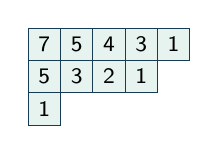
\begin{tikzpicture}[x=.41cm,y=-.41cm,baseline]
\foreach \i/\j/\h in {0/0/7,1/0/5,2/0/4,3/0/3,4/0/1,0/1/5,1/1/3,2/1/2,3/1/1,0/2/1}{\draw[draw=inkblue,fill=soft](\i,\j)rectangle ++(1,1);\node[font=\footnotesize\sffamily] at (\i+.5,\j+.5) {\h};}
\end{tikzpicture}
\end{minipage}\begin{minipage}{.58\linewidth}\small
Each box shows its hook length. The product for shape $(5,4,1)$ is $12{,}600$, so the theorem below gives $10!/12{,}600=288$ standard fillings.
\end{minipage}
\end{center}

\subsection{Corner recursion and the hook-length formula}

\begin{theorem}[Frame--Robinson--Thrall hook-length formula]\label{result15}
If \(f^\lambda\) counts the standard tableaux of shape \(\lambda\), then
\[
 f^\lambda \prod_{(i,j)\in\lambda} h_{ij}=n!.
\]
Transposition preserves \(f^\lambda\). For a rectangle with \(r\) rows
of length \(s\), the count is \((rs)!\prod_{j=0}^{r-1} j!/(s+j)!\).
For two rows of lengths \(a\ge b\) it is
\(\binom{a+b}b-\binom{a+b}{b-1}\), interpreting the second term as zero
for \(b=0\).
\end{theorem}
\begin{proof}
Put \(x_i=\lambda_i+r-i\), so \(x_1>\cdots>x_r\ge0\), and write
\(\Delta(x)=\prod_{i<j}(x_i-x_j)\). The hooks in row \(i\) are exactly
the numbers \(1,\ldots,x_i\) with the \(r-i\) numbers \(x_i-x_k\)
for \(k>i\) omitted. Indeed the row's hook lengths
\[
 h_{ij}=\lambda_i-j+1+\#\{k>i:\lambda_k\ge j\}
\]
strictly decrease with \(j\) and lie in that range. For \(k>i\), if
\(j\le\lambda_k\) the lower rows through \(k\) all contribute, giving
\(h_{ij}>x_i-x_k\). If \(j>\lambda_k\), at most \(k-i-1\) lower rows
contribute and \(h_{ij}<x_i-x_k\). The omitted numbers are distinct,
and \(x_i-(r-i)=\lambda_i\) accounts for all others. Multiplying the row
products gives
\[
 \prod_{(i,j)\in\lambda}h_{ij}=\frac{\prod_i x_i!}{\Delta(x)}.
\]

For \(n>0\), the largest tableau entry occupies a removable corner,
namely the last box in some row \(i\) with
\(\lambda_i>\lambda_{i+1}\), where \(\lambda_{r+1}=0\).
Deleting it and reattaching \(n\) give inverse bijections. Thus
\(f^\lambda=\sum_{i\ {\rm removable}} f^{\lambda-e_i}\) with
\(f^\varnothing=1\). We verify this recursion for the positive rational
number \(W(\lambda)=n!\Delta(x)/\prod_i x_i!\). For a removable row,
\[
 \frac{nW(\lambda-e_i)}{W(\lambda)}=x_i A_i,\qquad
 A_i=\prod_{j\ne i}\frac{x_i-x_j-1}{x_i-x_j}.
\]
This follows by dividing the two factorial products and the factors of
\(\Delta\) involving \(i\). A nonremovable row contributes \(x_iA_i=0\):
either \(i<r\) and \(x_i-x_{i+1}=1\), or \(i=r\) and \(x_i=0\).

We need \(\sum_i x_iA_i=\sum_i x_i-\binom r2=n\). Here is a finite
algebraic proof. Put \(P(X)=\prod_i(X-x_i)\). Then
\[
 P(X-1)=P(X)-\sum_i A_i\prod_{j\ne i}(X-x_j).
\]
The difference of the sides has degree at most \(r-1\) and vanishes at
each of the \(r\) distinct integers \(x_i\), by the defining product for
\(A_i\). A polynomial vanishing at \(u\) is divisible by \(X-u\),
by subtracting its value from each monomial; repeated cancellation
at the other roots proves the required degree bound on the number of
roots. Substitute \(X=1/t\), multiply by \(t^r\), and divide through
by \(\prod_i(1-x_it)\) in the ring \(\mathbb Q[t]/(t^3)\). The factors
are units with inverses \(1+x_it+x_i^2t^2\). This gives the equality
\[
 \prod_i\left(1-\frac{t}{1-x_i t}\right)
   =1-\sum_i A_i \frac{t}{1-x_i t}\pmod{t^3}.
\]
The quadratic coefficient on the left is \(\binom r2-\sum_i x_i\);
on the right it is \(-\sum_i A_i x_i\), as required. For the empty
shape the hook-product expression gives \(W=1\), also with padded
zero rows. The recursion now proves \(W=f^\lambda\) by induction on
\(n\), giving the stated integral identity.

Transposition exchanges the increasing conditions and is its own inverse.
For the rectangle \(x_i=s+r-i\); grouping differences by the smaller
coordinate gives \(\Delta=\prod_{j=0}^{r-1}j!\). For two rows
the shifted coordinates are \(a+1,b\), giving
\((a+b)!(a-b+1)/((a+1)!\,b!)\); expanding the two binomials gives this
same expression.
\end{proof}

\subsection{Semistandard tableaux and the hook-content formula}

\begin{theorem}[Hook-content formula]\label{result16}
For a shape with at most \(r\) rows let \(D_r(\lambda)\) count
semistandard fillings with entries in \(1,\ldots,r\). Then
\[
 D_r(\lambda)=\frac{\Delta(x)}{\prod_{k=0}^{r-1}k!}
 =\prod_{(i,j)\in\lambda}\frac{r+j-i}{h_{ij}}.
\]
For the shape \((5,4,1)\) there are \(288\) standard tableaux and
\(66{,}528\) semistandard tableaux on \(1,\ldots,7\).
\end{theorem}
\begin{proof}
Deleting the entries equal to \(r\) leaves a shape \(\nu\) of at most
\(r-1\) rows. Every such entry is at the right end of its row, in the
sense that all subsequent cells in the row also have entry \(r\).
Every box in row \(r\) must contain \(r\), by column strictness.
The possible shapes are exactly
\(\lambda_i\ge\nu_i\ge\lambda_{i+1}\) for \(1\le i<r\). Indeed the
boxes above row \(i+1\) of \(\lambda\) cannot be deleted. Conversely,
fill the difference of the two shapes with \(r\); the inequalities put
every added box below a retained box if an upper box exists, and place
no box below an added box. This extends every semistandard \(\nu\)
uniquely for that shape. In shifted coordinates
\(y_i=\nu_i+r-1-i\) this says the \(y_i\) range independently over
\(x_{i+1}\le y_i<x_i\). These inequalities already imply strict descent
of the \(y_i\).

For a descending list \(v\) of length \(l\), define
\[
 B_l(v)=\det\bigl(\binom{v_i}{l-j}\bigr)_{1\le i,j\le l}
       =\frac{\prod_{i<j}(v_i-v_j)}{\prod_{k=0}^{l-1}k!}.
\]
For the determinant evaluation, the polynomial \(\binom{X}{k}\) has
leading coefficient \(1/k!\), and the lower-degree monomials are already
spanned by the columns of lower degrees. Subtracting their multiples
successively reduces to the determinant of descending powers with
the displayed factorial factor. The latter determinant is \(\Delta(v)\):
as a polynomial in \(v_1\) it has roots \(v_2,\ldots,v_l\) by equal
rows, and leading coefficient the corresponding smaller determinant
by expansion along row one. The root argument just used above verifies
the factorization for fixed distinct lower entries, and induction gives
the formula. Empty determinants are one.

By induction with \(r-1\) symbols, the deletion count is the sum of
\(B_{r-1}(y)\) over the stated intervals. Expand the determinant as a
signed permutation sum and sum independently in each row. The result
is a determinant of row sums. Pascal's identity telescopes these sums:
\[
 \sum_{z=x_{i+1}}^{x_i-1}\binom zk
   =\binom{x_i}{k+1}-\binom{x_{i+1}}{k+1}.
\]
In the matrix for \(B_r(x)\), subtract row \(i+1\) from row \(i\)
for \(i=1,\ldots,r-1\) in that order. The determinant stays unchanged
by multilinearity and cancellation for repeated rows. Its constant
last column is now zero except for a final one. Expansion there gives
exactly the determinant of the above differences for
\(k=r-2,\ldots,0\). This proves the recurrence, with the empty shape
at \(r=0\) as base. Multiplying the factorials in each numerator row gives
\(\prod_{j=1}^{\lambda_i}(r+j-i)=x_i!/(r-i)!\). The row hook product
proved above gives the content formula. For the example the hook rows
are \(7,5,4,3,1;\ 5,3,2,1;\ 1\), with total product \(12600\).
The numerator is \(10!\) in the standard case and
\((7\cdot8\cdot9\cdot10\cdot11)(6\cdot7\cdot8\cdot9)5\)
in the semistandard case. Division gives the two values.
\end{proof}

\subsection{Permutation insertion and increasing subsequences}

\begin{theorem}[Robinson--Schensted correspondence and Schensted's first-row theorem]\label{result17}
Permutations of \(1,\ldots,n\) correspond bijectively to pairs \((P,Q)\)
of standard tableaux of the same shape \(\lambda\) of size \(n\).
The longest strictly increasing subsequence of the permutation has length
\(\lambda_1\), with length zero for the empty shape. Consequently
\[
  \sum_{\lambda\vdash n}(f^\lambda)^2=n!.
\]
The number of permutations avoiding an increasing subsequence of length
\(k+1\) is the same sum restricted to shapes with \(\lambda_1\le k\).
\end{theorem}
\begin{proof}
Build the insertion tableau \(P\) from the empty filling by reading
the permutation in order. To insert \(a\) in a row, find its leftmost
entry \(b>a\). If found, replace \(b\) by \(a\) and insert \(b\) in the
next row. Otherwise append \(a\) and stop. A missing row acts as empty.
The entries are distinct throughout. A replacement preserves row order,
and no column inequality with a lower neighbor is harmed by decreasing
the cell. If the bump out of a row occurs at column \(c\), its insertion
in the next row occurs at a column \(c'\le c\): the old entry there at
column \(c\), when present, exceeds the bumped value, and a shorter row
can append no later than \(c\). For the new entry at \(c'\) its upper
neighbor is smaller. When \(c'<c\) this follows from the old upper row's
strict order; when \(c'=c\) that neighbor was just replaced by a smaller
value. In particular an appended box in a lower row has an upper box.
The procedure visits at most one row past the old height and adds exactly
one corner. Put the insertion time in this new box in \(Q\). Every
immediately preceding box above or to its left existed earlier, so \(Q\)
is standard.

For the inverse, find the box of the largest remaining time in \(Q\).
It is removable. Delete it in both tableaux, carrying its value \(b\)
from \(P\). In the row above, use the \emph{rightmost} entry \(a<b\),
replace \(a\) by \(b\), and carry \(a\) upward. On passing above row
one, output the carried value. Such a choice always exists when a row
above remains: if the carried value came from column \(c\), that upper
row had a smaller entry at \(c\). The chosen column \(c'\) is therefore
at least \(c\). Replacing \(a\) by \(b\) preserves the row order by
the rightmost rule. Its upper neighbor stays smaller. For its lower
neighbor, the lower row's entry formerly at \(c\) was just deleted or
increased; at a chosen \(c'\ge c\), a lower entry if present now exceeds
the carried \(b\). This verifies all inequalities as the reverse path
proceeds. After any upward replacement, the entries to its left are
below the value \(a\) carried out, so the first entry exceeding \(a\) on
reinsertion is exactly the newly placed \(b\). In the bottom row the
deleted last entry simply appends on reinsertion. In the other direction,
after a forward bump, its replaced entry and all entries to its left
are smaller than the bumped value, and all entries to its right are
larger; the reverse search necessarily picks the same cell. Hence the
local procedures invert each other. Repeating deletions recovers the
permutation in reverse order: each deletion ejects exactly one distinct
label from the remaining set. This proves the bijection and its square sum.

To identify the first row, for a processed prefix call \(m_j\) the
least possible final value of an increasing subsequence of length \(j\),
whenever one exists. The first row after this prefix consists exactly
of these \(m_j\), in increasing order. Prove it by induction, starting
with the empty row. When a new distinct value \(a\) arrives, let \(c\)
be the first column with \(m_c>a\), or the next unused column if there
is none. A subsequence of length \(c\) now ends in \(a\): extend one
ending in \(m_{c-1}<a\) or use the singleton if \(c=1\). No longer
subsequence ending in \(a\) exists, since its prefix of length \(c\)
would have a last element smaller than \(a\), whereas the old \(m_c\)
was absent or larger. For smaller lengths the old minima are already
below \(a\). For greater lengths no new candidate is available. Thus
exactly column \(c\) is replaced or appended, as in the first-row
insertion rule. This proves the claim and the restricted sum.
\end{proof}

\begin{corollary}[Catalan permutation avoidance]\label{result18}
The number of permutations of length \(n\) avoiding an increasing
subsequence of length three is \(C_n\), and the same is true for avoiding
a decreasing subsequence of length three.
\end{corollary}
\begin{proof}
Transpose both tableaux of a pair whose common shape has at most two
columns. A standard tableau with at most two rows gives a length-\(n\)
path with up-steps for top-row labels and down-steps for bottom-row
labels, reading the labels in increasing order. Every prefix has at least
as many up-steps as down-steps, by column strictness. Conversely fill
the next vacant cell of the indicated row at each step; the prefix
condition ensures column strictness. Two such paths have equal final
height exactly when their shapes agree, because their lengths are equal.
Concatenate the first path with the second read backwards and with steps
negated. This gives a Dyck path of length \(2n\), and cutting at its
middle gives the two inverse paths. Reversing the positions in a
permutation interchanges increasing and decreasing subsequences. The
argument also includes \(n=0\).
\end{proof}

\paragraph{Arithmetic bounds and Lean obligations.}
For fixed size bound \(N\) and row count \(r\), take a shape code with
\(r\) digits in base \(\max(2,N+1)\). Tableaux can be stored in
\(rN\) entries, with zero padding; use base \(\max(2,N+1,r+1)\) for
both kinds. Define \texttt{isShape}, \texttt{inShape}, \texttt{isSYT},
\texttt{isSSYT}, \texttt{removable}, \texttt{hook} and
\texttt{shiftedRow} by bounded scans. For the hook identity take
induction on \(m\le N\) with a Boolean fold over all shape codes of
size at most \(m\). The corner proof locates \(m\), erases its cell,
and inverts this transformation by reattaching \(m\).
For \texttt{cornerWeightSum}, implement rational polynomial coefficients
with signed numerator and positive denominator and use arrays through
degree \(r\), plus length-three arrays for the truncated expansion.
The largest shifted coordinate is at most \(N+r\); every factorial in
the formulas is bounded by \((N+r)!\). For the semistandard induction
fix an alphabet bound \(R\) and size bound \(N\) and fold over all shapes
of size at most \(N\) with at most the current number of rows, using
padding to length \(R\). A determinant of size \(l\le R\) is the signed
sum over permutations, each checked in base \(\max(2,l)\). Prove row
linearity by distribution, repeated-row cancellation by swapping the two
row assignments, and cofactor expansion by the chosen column index and
the induced order on the remaining indices. These finite identities
suffice for the telescoping determinant proof.

For insertion take a padded \(N\times N\) tableau. Implement
\texttt{bump}, \texttt{unbump}, \texttt{insert} and \texttt{removeCorner}
with at most \(N+1\) row visits and at most \(N\) comparisons per row.
The local inverse invariant records the carried entry, the previous
column and the untouched prefixes or suffixes of the current and
adjacent rows. Apply the two local inverse lemmas along the stored
row path, then induct on the permutation prefix, retaining the shape
agreement and validity of both tableaux. For the subsequence invariant
enumerate index masks below \(2^N\) to define a least final value or an
absent marker for each length. These are primitive recursive observations
of a fixed finite prefix; the argument uses no quantification over
uncoded maps or infinite series.

\paragraph{Sources.}
The numerical examples appear on the seed's linked
\href{https://en.wikipedia.org/wiki/Young_diagram}{Young diagram/Young tableau}
page. The original papers give the hook formula and the subsequence
interpretation, respectively: J. S. Frame, G. de B. Robinson and R. M.
Thrall, \emph{The Hook Graphs of the Symmetric Group}
(\href{https://doi.org/10.4153/CJM-1954-030-1}{1954}), and
C. Schensted, \emph{Longest Increasing and Decreasing Subsequences}
(\href{https://doi.org/10.4153/CJM-1961-015-3}{1961}).

\section{Graphs, extremal problems and finite Ramsey theory}
\label{sec:graphs}

The survey asks how many graphs have a prescribed number of edges, which triangle-free graphs have the most edges, and how many triangles a random graph has on average. Its link to Hamiltonian cycles leads to statements about degree conditions and tournaments. We begin with these questions, then develop matching, tree enumeration and finite Ramsey theory as further results within the linked subjects.

\subsection{Counting graphs and local configurations}

Use $[n]=\{0,\ldots,n-1\}$. Enumerate the $M=\binom n2$ unordered pairs in lexicographic order. A simple graph $G$ is a mask below $2^M$, with a bit for each edge. Write $e(G)$ for its number of edges, $d(v)$ for a vertex degree and $t(G)$ for the number of unordered triangles. All counts use labeled vertices.

\begin{proposition}[Graph counts, handshaking and finite averages]\label{result19}
There are $2^M$ graphs on $[n]$ and $\binom Mk$ with $k$ edges. In each graph, $\sum_v d(v)=2e(G)$ and the number of vertices of odd degree is even. The mean of $t(G)$ over uniform masks is $\binom n3/8$. A graph with $e$ edges has a partition into two classes with at least $\lceil e/2\rceil$ crossing edges.
\end{proposition}
\begin{proof}
Selecting edges is exactly selecting a subset of the $M$ positions. Each edge has two ends, which proves the degree sum. Reducing that sum modulo two counts odd degrees modulo two. For $n\ge3$, fixing a triple and requiring its three edges leaves $M-3$ free bits. Summing first over triples, then over graphs, gives
\[
 8\sum_{G<2^M}t(G)=2^M\binom n3 .
\]
For $n<3$ both sides vanish. For the cut claim color the vertices with independent bits, meaning that we enumerate all $2^n$ masks. For each edge exactly half of the masks give its ends different colors, by toggling the first end. If $e>0$ the sum of the cut sizes is $e2^{n-1}$. The largest cut is at least the average and is returned by a mask scan. If $e=0$, any partition suffices.
\end{proof}

\subsection{The triangle-free extremum and its generalization}

For $r\ge1$ let $T_r(n)$ be a complete $r$-partite graph whose parts have sizes $q$ and $q+1$, where $n=rq+s$ and $0\le s<r$. There are $s$ larger parts. Empty parts are allowed. Its edge count is
\[
 t_r(n)=\binom n2-(r-s)\binom q2-s\binom{q+1}2 .
\]

\begin{theorem}[Tur\'an, including equality]\label{result20}\label{thm:graph-turan}
Every $K_{r+1}$-free simple graph on $n$ vertices has at most $t_r(n)$ edges. Equality holds precisely for graphs isomorphic to $T_r(n)$. In particular the triangle-free maximum is $\lfloor n^2/4\rfloor$, attained only by a complete bipartite graph with part sizes differing by at most one.
\end{theorem}
\begin{proof}
Among complete $r$-partite graphs on $n$ vertices the missing edges are the pairs within the parts. Moving one vertex from a part of size $a$ to a part of size $b$, with $a\ge b+2$, reduces the number missing by $a-b-1>0$. After at most $\binom n2$ moves the sizes differ by at most one. This proves the bound and its strictness for unbalanced partitions.

Induct on $r$. For $r=1$ the allowed graphs have no edges. For $r>1$ and $n>0$, take a vertex of maximum degree $d$, let $A$ be its neighborhood, and put $B=[n]\setminus A$. A clique of size $r$ in $A$ would extend to size $r+1$. Thus $e(A)\le t_{r-1}(d)$. Counting the edges with at least one end in $B$ gives
\[
 e(G)=e(A)+\sum_{b\in B}d(b)-e(B)
       \le t_{r-1}(d)+|B|d.
\]
The right side counts the edges of a complete $r$-partite graph formed by adjoining one part $B$ to $T_{r-1}(d)$. It is at most $t_r(n)$. In case of equality, $e(B)=0$, every $b\in B$ has degree $d$, and equality holds in $A$. Hence each $b$ is adjacent to all $d$ vertices of $A$, and the induction hypothesis splits $A$ into the required parts. Strictness of the balancing step makes all $r$ final parts balanced. Conversely the displayed $T_r(n)$ has no clique larger than $r$. For $n=0$ take all parts empty. For $r=2$ the product of the part sizes is $\lfloor n^2/4\rfloor$.

To use quantifier-free induction, fix an ambient bound $N$ for the number of vertices. The induction assertion for $r$ checks all $n\le N$, masks below $2^{\binom N2}$ and, in the equality case, the existence of a part assignment among the $r^n$ words. Relabel an induced graph by the increasing enumeration of its vertices. The check is a primitive recursive Boolean, including when $r>n$.
\end{proof}

\subsection{Hamiltonian cycles and tournaments}

A Hamiltonian path is a listing of all vertices without repetition with an edge between successive entries. A Hamiltonian cycle also uses the last-to-first edge. For undirected cycles assume $n\ge3$, and identify rotations and reversals. In $K_n$ there are $(n-1)!/2$ such cycles. Starting at vertex $0$ leaves $(n-1)!$ orderings, and reversal pairs them without a fixed point. For complete bidirected graphs with orientations distinguished the count is $(n-1)!$. For a Hamiltonian undirected graph, removing any one vertex from a cycle leaves a path spanning the remaining vertices. In particular it is biconnected.

\begin{theorem}[Bondy--Chv\'atal closure, Ore and Dirac]\label{result21}\label{thm:graph-closure}
Let $n\ge3$. Adjoin edges between nonneighbors whose degrees sum to at least $n$, until no such pair remains. The resulting closure is canonical and has a Hamiltonian cycle if and only if the original graph has one. In particular a Hamiltonian cycle can be found if every nonadjacent pair has degree sum at least $n$, or if $2d(v)\ge n$ for each vertex.
\end{theorem}
\begin{proof}
Consider a cycle after adding one edge $uv$. If it uses that edge, deleting it gives a Hamiltonian path $x_1=u,\ldots,x_n=v$ in the old graph. Among $1\le i<n$, mark red the indices with edge $ux_{i+1}$, and blue those with edge $x_iv$. The red and blue counts are $d(u)$ and $d(v)$, respectively. Their sum is at least $n$ on $n-1$ positions. The first doubly marked $i$ supplies the old cycle
\[
 x_1,\ldots,x_i,x_n,x_{n-1},\ldots,x_{i+1},x_1 .
\]
If the new cycle omits $uv$, it already works. Any old cycle persists after insertion. Store the at most $M$ inserted edges and undo them in reverse to reconstruct a certificate. Every saturated supergraph containing the input contains each inserted edge, by induction on insertions and monotonicity of degrees. Taking another terminal result as that supergraph and interchanging their roles proves uniqueness. Under Ore's hypothesis all missing pairs stay eligible, so the closure is complete. Dirac's condition implies Ore's by adding the two degree inequalities.
\end{proof}

A tournament orients each unordered pair in exactly one direction. For a loopless digraph $D$, let $h(D)$ count the vertex listings forming directed Hamiltonian paths. Its complement $\overline D$ reverses the presence of each nonloop ordered pair.

\begin{theorem}[Berge parity, R\'edei and Camion]\label{result22}\label{thm:graph-tournaments}
One has $h(D)\equiv h(\overline D)\pmod2$. Every tournament has an odd number of Hamiltonian paths. A tournament on $n\ge3$ vertices has a directed Hamiltonian cycle precisely when it is strongly connected.
\end{theorem}
\begin{proof}
For $n\ge1$ count pairs consisting of a vertex listing and a subset of its consecutive directed arcs belonging to $D$. A listing with $j$ such arcs contributes $2^j$, odd exactly when the listing is a path of $\overline D$. Conversely, any prescribed marked set which occurs forms disjoint directed paths, including isolated vertices as one-vertex paths. With $b$ such blocks it occurs in exactly $b!$ listings, by permuting the blocks. Only $b=1$ gives an odd count, and those marked sets are exactly the full Hamiltonian paths in $D$. This proves Berge's congruence. For $n=0$ the empty listing contributes one on each side.

Reverse one arc in a tournament $T$ to get $T'$. Let $D_0$ omit both orientations of the pair and $D_2$ include both. Paths avoiding the pair are counted twice in $h(T)+h(T')$, and paths using it are counted once. Thus $h(T)+h(T')=h(D_0)+h(D_2)$. The reverse of $D_2$ is $\overline D_0$. Reversing a listing preserves the path count under reversal of all arcs. By Berge the right side is even. Reverse all arcs pointing from a larger to a smaller label, in at most $M$ steps. The resulting tournament has just the increasing Hamiltonian path, proving oddness. A bounded listing search now returns a path.

A directed Hamiltonian cycle gives a directed route between every ordered pair. Conversely, in a strongly connected tournament on at least three vertices, any arc followed by a shortest return path gives a simple directed cycle. Select a longest simple cycle $C$ by scanning vertex words of length at most $n$. For any vertex $z$ off $C$, if the edges from $C$ to $z$ have both orientations then two consecutive cycle vertices satisfy $c_i\to z\to c_{i+1}$, allowing insertion. Consequently all outside vertices lie in two classes, $A$ with $C\to A$ and $B$ with $B\to C$. If any outside vertices exist, both classes must occur, as otherwise reachability in one direction fails. Some arc $a\to b$ must run from $A$ to $B$, since otherwise $A$ cannot reach $C$. Replacing an edge $c_i\to c_{i+1}$ by $c_i\to a\to b\to c_{i+1}$ contradicts maximality. Hence $C$ spans. Every choice just used is a finite first or maximum.
\end{proof}

\begin{proposition}[The Petersen graph]\label{result23}
The Petersen graph is cubic, biconnected and of diameter two and girth five. It has no Hamiltonian cycle.
\end{proposition}
\begin{proof}
Use labels $O_i,I_i$ for $i$ modulo five. Join $O_i$ to $O_{i+1}$, $I_i$ to $I_{i+2}$ and $O_i$ to $I_i$ for each $i$. Each layer is a 5-cycle and every vertex has one spoke to the other layer. After deleting one vertex the intact layer and the path in the other layer remain joined by spokes. Two vertices in one layer are within two steps. For a pair in different layers, differences $0,\pm1,\pm2$ are covered by a spoke alone or a spoke with one outer or inner edge. Some pairs are nonadjacent, giving diameter two. A simple cycle using both layers uses a positive even number of spokes, separated by at least one layer edge. A cycle of length at most four would have exactly two spokes and one edge in each layer. Their indices would have to differ both by $\pm1$ and by $\pm2$, which is impossible modulo five. Either layer attains girth five.

A Hamiltonian cycle must use two or four spokes. With two, each layer supplies a spanning path in its 5-cycle, so its two spoke indices are adjacent in both layer cycles, again impossible. With four, rotate labels so that spoke zero is omitted. Both outer edges at $O_0$ are forced, leaving $O_2O_3$ forced since $O_1,O_4$ already have two chosen incidences. Both inner edges at $I_0$ are also forced. Consequently the purported Hamiltonian cycle already contains the closed 5-cycle $O_2,O_3,I_3,I_0,I_2,O_2$. A simple cycle containing this closed component cannot visit its other five vertices.
\end{proof}

\subsection{Cayley graphs and change ringing}

A finite group is an explicitly verified multiplication table on $[g]$ with identity and inverse table. Given $S\subseteq G$, put a directed arc of color $s$ from $x$ to $xs$ for each $s\in S$. Forgetting colors gives its Cayley digraph. An action of $G$ on a nonempty vertex set is \emph{simply transitive} if for each ordered pair of vertices exactly one group element takes the first to the second.

\begin{theorem}[Finite Cayley graphs and Sabidussi's characterization]\label{result24}
Every vertex has indegree and outdegree $|S|$. Left multiplication acts simply transitively by color-preserving automorphisms. When $S$ generates $G$, all color-preserving digraph automorphisms arise this way. The components of the underlying undirected graph are the left cosets of $\langle S\rangle$. A finite nonempty digraph given by a Boolean adjacency relation (loops allowed) admits a simply transitive action of $G$ by automorphisms precisely when it is isomorphic to a Cayley digraph of $G$ for some $S$.
\end{theorem}
\begin{proof}
From $x$ the outgoing ends $xs$ are distinct by cancellation, and the incoming starts $xs^{-1}$ are distinct for the same reason. Translation by $h$ takes $x\to xs$ to $hx\to(hx)s$ preserving color, and $yx^{-1}$ is the unique translator sending $x$ to $y$. Along an undirected walk, each step is right multiplication by an element of $S$ or its inverse. Conversely such a word gives a walk. Hence vertices reachable from $x$ form $x\langle S\rangle$. All connectivity and subgroup membership tests may use walks of length less than $g$, by erasing repeated-vertex segments. If $S$ generates and an automorphism sends the identity to $h$, it must propagate $x\mapsto hx$ along every one of these steps, because each color has a unique incoming and outgoing neighbor. Hence it is left translation.

Conversely fix a vertex $v$ of a supplied simply transitive action. The map $a\mapsto av$ is bijective, and inverse images are found by scanning $[g]$. Set $S=\{s:v\to sv\}$. Applying $a^{-1}$ to an arc shows that $av\to bv$ holds exactly when $a^{-1}b\in S$. Thus the bijection identifies the original edges with the Cayley edges. This form allows a non-generating $S$ when the digraph is disconnected.
\end{proof}

\begin{proposition}[Two cyclic Gray listings]\label{result25}
The $d$-dimensional cube has a Hamiltonian cycle for $d\ge2$. The Cayley graph of the symmetric group on $n\ge3$ letters with adjacent position swaps as generators also has a Hamiltonian cycle.
\end{proposition}
\begin{proof}
For binary words start with $0,1$. Given a listing, prefix $0$ to it in forward order and append its reverse prefixed by $1$. The transition between the halves switches only the new bit. The final and initial words also differ at that bit. Within a half the old adjacency survives, and deletion of the prefix identifies the old word uniquely. Iteration lists all $2^d$ words and gives a simple cycle for $d\ge2$.

For permutations begin with $12,21$, whose last and first entries are adjacent by one swap. Given the old cyclic listing on $n-1$ letters, replace each word by a row of $n$ words inserting the new letter $n$ in all positions. In the first row move $n$ from the right end to the left end, in the second from left to right, and continue alternating. Inside a row the step is adjacent. Between rows the letter $n$ stays at one end and the old words differ by an adjacent swap. There are $(n-1)!$ rows, an even number for $n\ge3$, so the final row ends with $n$ on the right, just as the first row began. The old closing swap therefore closes the new listing. Deleting $n$ identifies its row and its position identifies its place within that row, so all $n!$ permutations appear exactly once. These recursions construct both cyclic listings from the dimension or alphabet size.
\end{proof}

\subsection{Euler trails and labeled trees}

\begin{proposition}[Euler's criterion]\label{result26}
In a finite undirected multigraph with at least one edge, there is a closed trail using every edge once if and only if the positive-degree vertices are connected and all degrees are even. There is an open such trail if and only if the same support is connected and exactly two degrees are odd.
\end{proposition}
\begin{proof}
Give each edge its own index and count a loop twice at its vertex. On a trail, arrivals and departures pair at every internal visit, leaving just the endpoints unpaired for an open trail. All used vertices lie in a single component. In the even case start at an incident vertex and repeatedly use the least unused incident edge. A stop away from the starting point would leave an odd number of used incidences there and hence a positive odd number unused. The trail therefore closes. Its removal leaves even degrees. If edges remain, some vertex of the trail is incident with a remaining edge. Otherwise the trail vertices, which contain both ends of every used edge, would be separated from all remaining edges in the original support. Construct another closed trail there and splice it at that vertex. Each splice uses at least one more edge and the total number of edge choices over all rounds is the initial edge count. In the two-odd case temporarily add one distinguished edge joining those vertices, find the closed trail and cut it at that edge. Connectivity tests need only paths with at most $n-1$ edges, since a repeated-vertex segment can be deleted.
\end{proof}

\begin{theorem}[Pr\"ufer coding and Cayley's formula]\label{result27}\label{thm:graph-prufer}
On $[n]$, $n\ge2$, the labeled trees are in primitive recursive bijection with the $n^{n-2}$ words of length $n-2$ over $[n]$. For $d_i\ge1$ with $\sum_i d_i=2n-2$, exactly
\[
 \frac{(n-2)!}{\prod_{i<n}(d_i-1)!}
\]
of the trees have degrees $d_i$. There is one tree on one labeled vertex.
\end{theorem}
\begin{proof}
A tree is connected and has no simple cycle. When it has at least two vertices, the two ends of a longest simple path have degree one. Indeed an extra neighbor of an endpoint would extend the path or close a cycle. Deleting a leaf preserves connectedness of the remaining vertices, since a simple path between them cannot pass through a leaf. It also preserves acyclicity. Thus a tree on $n\ge1$ vertices has $n-1$ edges, by deleting leaves down to one vertex.

Repeatedly delete the least leaf and record its sole neighbor until two labels remain. In the resulting word each label $v$ occurs $d(v)-1$ times. Its degree drops by one every time it is recorded, and reaches one either at its own deletion or at the final pair. This argument applies to every suffix of the process.

Given a word, keep all labels live. With $m\ge3$ live labels the suffix has length $m-2$ and consists entirely of live labels. Choose the least live label $u$ missing from the suffix, join it to the first letter, retire $u$ and erase the first letter. At least two live labels are missing, and the first letter differs from $u$. Join the last two labels. Reading the construction backwards attaches one new leaf at each stage, giving a tree. At any decoding stage a live label is used once when it retires (or in the final pair) and once per occurrence in the suffix. Thus the leaves of that residual tree are exactly the live labels missing from the suffix. The encoder therefore makes the decoder's choices on a decoded tree. Conversely the degree-count observation on an encoded tree makes the decoder follow its deletions step for step. Finally, prescribing the multiplicities $d_i-1$ in the word amounts to distributing its positions into labeled fibers of those sizes, giving the multinomial above by ordering and forgetting within-fiber order. All loops have at most $n$ steps.
\end{proof}

\subsection{Matching, deficiency and vertex covers}

Let $G\subseteq L\times R$ be bipartite, with $|L|=a$ and $|R|=b$. A matching is an edge subset in which no two edges share an endpoint. A vertex cover meets every edge. For $S\subseteq L$ put $N(S)=\{y\in R:(\exists x\in S)\,xy\in G\}$.

\begin{theorem}[K\H{o}nig, Hall and the deficiency formula]\label{result28}\label{thm:matching-cover}
One can construct a maximum matching $P$, a minimum cover $C$ and a set $S\subseteq L$ such that
\[
 |C|=|P|,\qquad a-|P|=|S|-|N(S)|
     =\max_{U\subseteq L} (|U|-|N(U)|).
\]
In particular a matching saturating $L$ exists exactly when $|N(U)|\ge |U|$ for every $U\subseteq L$. Failure yields a specific violating $U$.
\end{theorem}
\begin{proof}
Start with the empty matching. Direct every unmatched edge from left to right and every matched edge from right to left. From the set $F$ of unmatched left vertices compute the reachable sets $X\subseteq L$, $Y\subseteq R$, closing under directed edges for $a+b$ rounds. Reachable vertices have witnesses of length at most $a+b-1$ when the vertex set is nonempty, by deleting repetitions. If an unmatched right vertex is reached, take a shortest witnessing path. Its edges alternate between unmatched and matched, with unmatched first and last. Toggling the edges on this simple path preserves matching at interior vertices and matches the endpoints, increasing the size by one. Run at most $\min(a,b)$ augmentations. After this many successes a full smaller side rules out further paths, so one final reachability calculation always yields a terminal stage.

At that stage all of $Y$ are matched. Their mates are in $X\setminus F$, and every $x\in X\setminus F$ was reached through its unique matched edge. Thus matching gives a bijection $Y\longleftrightarrow X\setminus F$. Also $Y=N(X)$. An unmatched edge from $X$ leads to $Y$, and the matched neighbor of any matched $x\in X$ was already reached. Every $y\in Y$ was reached from a neighbor in $X$. It follows that $C=(L\setminus X)\cup Y$ covers all edges and
\[
 |C|=a-|X|+|Y|=a-|F|=|P|.
\]
Every cover meets the disjoint edges of any matching at distinct vertices. This proves that both displayed objects are optimal. For every $U$, the matched vertices in $U$ inject into $N(U)$, and its unmatched vertices number at most $|F|$. Thus $|U|-|N(U)|\le |F|$, with equality at $S=X$. The empty subset ensures the maximum is nonnegative. Taking $|F|=0$ gives Hall's criterion and taking $|F|>0$ gives its failure certificate.
\end{proof}

\begin{corollary}[Regular bipartite graphs, edge coloring and transversals]\label{result29}
A $d$-regular finite bipartite graph with $d>0$ splits into $d$ perfect matchings. Every finite bipartite graph of maximum degree $d$ admits a proper edge coloring with $d$ colors. A finite family $(A_i)_{i<a}$ of finite subsets of a common coded universe has a system of distinct representatives if and only if $|\bigcup_{i\in U} A_i|\ge |U|$ for every $U\subseteq[a]$.
\end{corollary}
\begin{proof}
Counting ends on each side gives $da=db$, so $a=b$ when $d>0$. Counting the $d|U|$ incident edges gives $d|U|\le d|N(U)|$, even with parallel edges counted with multiplicity. Hall returns a perfect matching. Remove it and iterate, lowering each degree by one. With parallel edges, apply Hall to the underlying simple graph and take the least available edge for each chosen pair. For edge coloring, add isolated dummy vertices to equalize the two sides. The sums of degree deficits from $d$ now agree. Repeatedly add one edge between a left and a right vertex of positive deficit, permitting parallel edges, until both sums are zero. At most $d\max(a,b)$ additions suffice. Color the resulting perfect matchings differently, then restrict to the original edges. For $d=0$ the empty coloring suffices. The representative assertion is Hall applied to the incidence edges $i\,y$ with $y\in A_i$.
\end{proof}

\begin{theorem}[Integral max-flow min-cut]\label{result30}
In a finite directed network with nonnegative integer capacities, distinct source $s$ and sink $t$, a maximum integral flow and a cut of equal capacity can be found by primitive recursion.
\end{theorem}
\begin{proof}
Index the arcs, allowing parallel arcs. A flow assigns each arc an integer between zero and its capacity, and balances inflow and outflow at every vertex other than $s,t$. Its value is net outflow at $s$. For a set $S$ containing $s$ and excluding $t$, summing the balance equations shows that net flow out of $S$ is the value, and is at most the sum of capacities of arcs leaving $S$.

Start with zero flow. Give each arc two indexed residual moves, forward with capacity $c-f$, backward with capacity $f$. Search for a simple $s$--$t$ path of positive moves (length at most $n-1$), recording move indices to distinguish parallel arcs. If found, augment by the least residual capacity on it. Bounds on all flows persist, intermediate vertices retain balance and the value increases by a positive integer. The value is bounded by the capacity $C_s$ out of $s$, so $C_s$ augmentations and a final residual search suffice. At termination, let $S$ be the set reachable by positive moves from $s$. Every arc leaving $S$ is full and every arc entering it has flow zero. The equality of the cut capacity and the flow value now proves optimality. Negative intermediate expressions can equivalently be represented by differences of two natural sums.
\end{proof}

\subsection{Ramsey bounds and a sum-free subset}

\begin{theorem}[Two-color graph Ramsey bounds]\label{result31}\label{thm:graph-ramsey}
For $s,t\ge1$, every red--blue coloring of the edges of $K_N$ with
\[
 N\ge B(s,t)=\binom{s+t-2}{s-1}
\]
has a red $s$-clique or a blue $t$-clique, with a primitive recursive witness. The least such size $R(s,t)$ is a primitive recursive function. In particular $R(3,3)=6$.
\end{theorem}
\begin{proof}
The boundary value $B(1,t)=B(s,1)=1$ suffices for a singleton. At an interior pair, Pascal gives $B(s,t)=B(s-1,t)+B(s,t-1)$. Among the other $N-1$ vertices a pivot has at least $B(s-1,t)$ red neighbors or at least $B(s,t-1)$ blue ones. Take a sufficiently large color class, recurse with the corresponding coordinate decreased, and extend a clique of the pivot's color by the pivot if needed. The measure $s+t$ decreases until the boundary. To express the argument by Boolean induction fix original $s_0,t_0$ and use the rectangle $s\le s_0,t\le t_0$ and all induced colorings relabeled on at most the original number of vertices. The finite conjunction of all previously reached cases with smaller coordinate sum is available as an induction invariant. Alternatively extract the recursive witness by storing the chosen pivots and unwinding.

For each $n\le B(s,t)$, scan all $2^{\binom n2}$ colorings and all subsets to test the Ramsey property and take the first success. Monotonicity follows by restriction. For $(3,3)$ the upper bound is six. Color the edges of a pentagon red and its diagonals blue. The two color graphs are 5-cycles (the blue cycle steps by two modulo five), so neither has a triangle.
\end{proof}

\begin{theorem}[Finite multicolor hypergraph Ramsey theorem]\label{result32}\label{thm:graph-hyperramsey}
For positive integers $j,c,m$ there is a uniform primitive recursive bound $H_j(c,m)$ and a primitive recursive procedure which, for every $c$-coloring of the $j$-subsets of a set of at least $H_j(c,m)$ vertices, selects $m$ vertices all of whose $j$-subsets have the same color. When $j>m$ this condition is vacuous. The least size with this property is itself primitive recursive.
\end{theorem}
\begin{proof}
Use $H_1(c,m)=c(m-1)+1$. Pigeonhole gives $m$ vertices of one color. Given $L=H_j(c,m)$ put
\[
 H_{j+1}(c,m)=(c+1)^{(L+1)(2^L+1)}.
\]
Order the input by its vertex labels. Build $L$ pivots $x_1<\cdots<x_L$, retaining a nonempty pool of larger unused vertices. Pick the least current vertex and delete it. For every $j$-subset $A$ of the chosen pivots whose last vertex is this new pivot, partition the current pool by the color of $A\cup\{y\}$ and retain a largest class, breaking ties by least color. Record this color $g(A)$. Across each round there is one deletion and at most $2^L$ thinnings. From a pool of size at least $(c+1)^h$ for $h\ge1$, either a single deletion or a largest-class thinning leaves at least $(c+1)^{h-1}$ vertices. Thus the exponent budget allows all rounds with vertices to spare. All later pivots come from every earlier retained pool. Hence for $i_1<\cdots<i_{j+1}$ the input color on those pivots equals $g(\{x_{i_1},\ldots,x_{i_j}\})$.

Apply the rank-$j$ result to the table $g$ on the $j$-subsets of the $L$ pivots and lift the selected $m$ positions. Every $(j+1)$-subset takes the common $g$-color of its first $j$ vertices. If there are no such subsets the assertion holds with any color. This proves the step. The displayed recursion is ordinary primitive recursion on rank. For the induction in iPRA, fix a target rank $h$ and put $N=H_h(c,m)$. These bounds are nondecreasing with rank. Code colorings on at most $N$ vertices as $2^N$ base-$(c+1)$ digits indexed by subset masks. For each rank $j\le h$ the assertion for every coloring on precisely $H_j(c,m)$ vertices with an $m$-set witness is a bounded Boolean test, using table codes below $(c+1)^{2^N}$ and witness masks below $2^N$. Perform induction on this test. Restrict larger inputs to their first $H_j(c,m)$ vertices. A least good size is obtained by bounded search through $H_h(c,m)$.
\end{proof}

For possibly different positive requested sizes $m_1,\ldots,m_c$, take $m=\max_i m_i$ and keep the first $m_i$ vertices of the returned set of color $i$. Schur's finite theorem follows already from rank two. If $[1,N]$ has $c$ colors, color $\{a,b\}\subseteq\{0,\ldots,N\}$ by the color of $|a-b|$. When $N+1\ge H_2(c,3)$ a monochromatic triangle $a<b<d$ gives the same color to $b-a,d-b,d-a$, and the first two sum to the third.

\begin{proposition}[A finite first-moment lower bound]\label{result33}
If $2\le k\le n$ and $2\binom nk<2^{\binom k2}$, there is a two-color edge coloring on $[n]$ with no monochromatic $k$-set. A bounded search returns one, so $R(k,k)>n$.
\end{proposition}
\begin{proof}
For each $k$-set precisely $2\cdot 2^{M-\binom k2}$ colorings make its edges monochromatic. The two choices of color are disjoint because $k\ge2$. Multiplying by $\binom nk$ counts the pairs (coloring, bad set), and the hypothesis says this is less than the number $2^M$ of colorings. If all colorings had a bad set, assigning the first one to each would give at least $2^M$ pairs. Equivalently the row counts have a zero, found by the first-success scan.
\end{proof}

\begin{theorem}[Erd\H{o}s's sum-free subset bound]\label{result34}\label{thm:graph-sumfree}
Every nonempty finite set $A$ of nonzero integers has a computably selected subset $B$ with $3|B|>|A|$ in which $x+y=z$ has no solution $x,y,z\in B$, even allowing repetitions.
\end{theorem}
\begin{proof}
Let $M=\max_{a\in A}|a|$ and $D=3M!-1$, with $M!$ denoting the factorial of $M$. The number $D\ge2$ is $2$ modulo $3$. Divide it repeatedly by its least divisor greater than one, found by search up to the current residual. Each divisor is prime, since a proper factor would be a smaller divisor. At most $D$ divisions produce a prime factorization. Some prime factor $p$ is $2$ modulo $3$, for no factor can be $3$ and a product of residues $1$ is $1$. Also $p>M$, as every prime $\le M$ divides $M!$ and cannot divide $3M!-1$.

Write $p=3q+2$. The $q+1$ residues $I=\{q+1,\ldots,2q+1\}$ are sum-free modulo $p$. Before reduction their pair sums lie from $2q+2$ to $4q+2$. After reduction they lie either above $2q+1$ or at most $q$. For $1\le t<p$ put $B_t=\{a\in A:ta\bmod p\in I\}$. Additivity modulo $p$ makes $B_t$ sum-free in the integers. Each $a$ is nonzero modulo $p$, so multiplication by $a$ permutes the nonzero residues. For clarity, the Euclidean algorithm on $p$ and the positive residue $a'$ obtains gcd $1$ since $p$ is prime. Tracking the coefficients in each remainder equation expresses $1$ as a linear combination of $a'$ and $p$, giving the inverse modulo $p$. The remainder decreases each round, so $p$ rounds suffice for the primitive recursion updating the coefficients. Thus $a$ is counted in exactly $q+1$ of the sets $B_t$. Consequently
\[
 3\sum_{1\le t<p}|B_t|=3|A|(q+1)>|A|(p-1).
\]
Take the first multiplier attaining the largest size. Its subset satisfies the asserted strict inequality. The factorial bound is deliberately elementary and covers $M=1$ with $p=2$.
\end{proof}

\subsection{Lean construction for the graph results}

The file \texttt{lean/Handshaking.lean} checks four uniform results with Lean's kernel. The proof of \texttt{transpose\_sum} inducts on the first side of a rectangle and distributes a prefix sum over addition. For \texttt{weighted\_handshaking}, adjoining vertex $n$ contributes a column and a row. Symmetry equates them and the new diagonal entry vanishes. The theorem \texttt{handshaking} specializes this identity to a natural-number graph mask. Its binary reader computes parity and the quotient by two by primitive recursion, with a proof of $2\lfloor x/2\rfloor+(x\bmod2)=x$. Finally \texttt{odd\_degree\_count\_even} supplies the half-count witnessing evenness. Lean reports no axiom dependencies for any of the four theorems. These are proofs about natural numbers in Lean. Their numerical specializations use equality induction on the prefix length, vertex count, or parity-recursion argument, as in the iPRA proofs above.


Use natural-number parameters for all finite domains. Define \texttt{edge n G u v} by the bit at the lexicographic rank of the ordered pair $(\min(u,v),\max(u,v))$, returning false outside $[n]$ or on the diagonal. Implement \texttt{degree}, \texttt{edgeCount} and \texttt{neighbors} as masked counts or folds. For digraphs reserve bit $nu+v$. A bipartite adjacency table uses bit $bx+y$. A vertex list uses digits $v+1$ in base $n+2$ together with its length. \texttt{simplePath}, \texttt{cycle}, \texttt{tree}, \texttt{matching}, \texttt{covers}, \texttt{clique} and \texttt{homogeneous} are bounded tests. They decode in-range labels and fold conjunctions for the required distinctness, incidences and colors. In \texttt{tree}, use connectivity by closure and reject simple cycles of lengths $3$ through $n$. For directed multigraphs paths also store the arc index and orientation of each step.

\begin{enumerate}
\item Prove that a bounded left fold computing reachable masks contains exactly the endpoints of walks of at most that many steps. Prove walk shortening by cutting the segment between the first repeated pair of positions. Store a predecessor on first discovery to implement path recovery, or return the least valid bounded word.
\item For \texttt{closeGraph}, iterate $\binom n2$ one-edge insertions with a no-op on saturation. Verify \texttt{repairCycle} from the double-marked path index, then unwind the recorded insertions. For tournaments, enumerate marked arc subsets and permutations for the parity lemma. The compatibility predicate for a marked set tests that each of its arcs is consecutive in the listing. Permuting its maximal path blocks is the inverse of cutting a compatible listing at unmarked gaps.
\item For \texttt{augment}, represent the matching as an edge mask. Prove the degree-at-most-one condition for toggling a simple alternating path by its endpoint/interior incidence counts. Then prove the terminal mate bijection, the cover test and cardinality equality from those masks. The flow version uses an array of arc flows with base one greater than the largest capacity (or base two if all capacities are zero). A bound for a path word uses the number of indexed residual moves.
\item For \texttt{pruferEncode} and \texttt{pruferDecode}, iterate exactly $n-2$ deletions. The invariant for their composition identifies the live mask and the residual tree and equates its live degrees with one plus the occurrence counts in the suffix. Induct on the number of processed letters and use the last-two-label base case. For Tur\'an, implement part assignments as bounded words and formalize the maximum-degree split followed by the strict decrease in within-part pairs.
\item For Ramsey, define $H$ by \texttt{Nat.rec} on rank, define the homogeneous-set witness by a bounded scan and verify the scan succeeds using the pivot invariant. The induction predicate quantifies only over the codes specified in the proof. At each round of the sum-free construction the data are integers encoded by signed naturals, a residual, a trial divisor, or a mask of the input set. The product-of-factors invariant and the residue double count are the two independent lemmas.
\end{enumerate}

The graph source pages are \href{https://en.wikipedia.org/wiki/Graph_theory}{Graph theory} as well as \href{https://en.wikipedia.org/wiki/Cayley_graph}{Cayley graph} and the directly linked \href{https://en.wikipedia.org/wiki/Hamiltonian_cycle}{Hamiltonian cycle} (redirecting to \emph{Hamiltonian path}). The overview's graph, extremal and probabilistic sections motivate the counting and extremal results. The one-third question is also explicit in \href{https://en.wikipedia.org/wiki/Extremal_combinatorics}{Extremal combinatorics}. Primary references for the closure and tournament subjects include \href{https://doi.org/10.1016/0012-365X(76)90078-9}{Bondy and Chv\'atal, \emph{A method in graph theory}} and \href{https://arxiv.org/abs/2307.05569}{Grinberg and Stanley, \emph{The R\'edei--Berge symmetric function of a directed graph}}.

\section{Order, incidence, and extremal set systems}
\label{sec:order-structure}

The survey asks for the largest antichain and the largest intersecting uniform
family on an \(n\)-element set. The answers use two different ways to read
a permutation: take its prefixes, or wrap it around a circle. We develop
the order-theoretic results first. Throughout, a subset of \([n]=\{0,\ldots,n-1\}\)
is a binary mask, a family is a mask of masks, and a poset on \([m]\) is
a reflexive, antisymmetric, transitive Boolean table. An integer can be
coded by a sign and an absolute value, with one code for zero.

\subsection{Chains, antichains, and finite lattices}

\begin{theorem}[Linear extensions and Mirsky's theorem]\label{result35}
A finite poset has a computable linear extension. Its maximum chain size
equals the minimum number of antichains partitioning it. Both extrema
come with witnesses.
\end{theorem}
\begin{proof}
For \(x\), let \(d(x)\) be the number of its weak predecessors. If \(x<y\),
the predecessor mask of \(x\) is properly included in that of \(y\), with
\(y\) witnessing properness. Thus \(d(x)<d(y)\). Sort by \((d(x),x)\)
lexicographically to get a linear extension. Read it in order and write
\[
 h(x)=1+\max(\{0\}\cup\{h(z):z<x\}).
\]
Induction on the processed prefix proves simultaneously that every chain
ending at a processed \(x\) has at most \(h(x)\) elements and that a chain
of exactly this size exists. For the upper bound, remove the endpoint
of a nonsingleton chain. For the lower bound append \(x\) to the recorded
chain at the first maximizing predecessor, using the singleton when the
predecessor set is empty. Strict comparison increases \(h\), hence every
nonempty fiber is an antichain. A longest chain meets distinct fibers
and needs a different part for each element in any antichain partition.
For the empty poset both numbers are zero. Chains are arrays of at most
\(m\) distinct labels; testing the upper-bound invariant amounts to a
bounded scan of padded arrays over \([m+1]\).
\end{proof}

\begin{theorem}[Dilworth's theorem]\label{result36}
The largest size of an antichain is the least number of chains partitioning
a finite poset. A partition and an antichain of the same size can be constructed.
\end{theorem}
\begin{proof}
On two copies of \([m]\) put the bipartite edges \(x_Ly_R\) with \(x<y\).
The matching and cover algorithm of Theorem~\ref{thm:matching-cover}
produces a matching and a vertex cover of the same size \(e\).
Treat each matched edge as an arrow \(x\to y\) on the original labels.
Each vertex has at most one incoming and one outgoing arrow. Each arrow
strictly increases \(d\), so following predecessors reaches a start
within \(m\) steps, and following successors from all starts partitions
the vertices into chains. There are \(m-e\) starts because exactly \(e\)
vertices have a predecessor. Keep labels \(x\) for which neither copy
belongs to the cover. At most \(e\) distinct labels were discarded.
Two kept labels cannot satisfy \(x<y\), since their edge would miss the
cover. This gives an antichain of size at least \(m-e\), and no antichain
can meet one of the constructed chains twice. These two witnesses
also certify both optimality claims.
\end{proof}

\begin{corollary}[Erd\H{o}s--Szekeres]\label{result37}
A list of \(rs+1\) pairwise distinct elements of a coded decidable linear order has a strictly increasing
subsequence of length \(r+1\) or a strictly decreasing one of length \(s+1\).
\end{corollary}
\begin{proof}
For each position \(i\) record the longest increasing and decreasing
subsequences ending there using the preceding recurrence over earlier
positions with smaller or larger value, respectively. If \(i<j\), either
the first length increases strictly from \(i\) to \(j\), or the second
does. All pairs of lengths differ. If all first lengths are at most \(r\)
and all second lengths at most \(s\), there are only \(rs\) pairs of
positive lengths. The pigeonhole count rules this out; scan for the first
excess and recover a subsequence from its predecessor pointers.
\end{proof}

\begin{theorem}[Finite distributive lattice representation]\label{result38}
A nonempty finite distributive lattice \(L\) is isomorphic to the lattice
of downward closed subsets of its poset \(J\) of nonzero join-irreducibles.
The isomorphism, its inverse, and \(J\) are primitive recursive in the
supplied join and meet tables.
\end{theorem}
\begin{proof}
The order is \(u\le v\) when \(u\vee v=v\); the bottom \(0_L\)
is the meet of all elements. A nonzero \(j\) belongs to \(J\) when
\(j=u\vee v\) always implies \(j=u\) or \(j=v\), a test over table indices.
Write \(I_x=\{j\in J:j\le x\}\). Every \(x\) is the join of \(I_x\)
(the empty join is \(0_L\)). Prove this in the linear extension:
for \(0_L\) and for \(x\in J\) it follows immediately. Otherwise a bounded
scan supplies \(x=u\vee v\) with \(u,v<x\); insert the two earlier
decompositions. Their terms all belong to \(I_x\), and all elements of
\(I_x\) lie below \(x\).
Distributivity makes each \(j\in J\) join-prime: if \(j\le u\vee v\)
then \(j=(j\wedge u)\vee(j\wedge v)\), so one summand equals \(j\).
Iteration gives the same conclusion for a nonempty finite join; a
nonzero \(j\) cannot lie below an empty join. For a downward closed
\(D\subseteq J\), put \(x=\bigvee D\). Then \(D\subseteq I_x\) and
each \(j\in I_x\) is below a member of \(D\), hence belongs to \(D\).
We have both inverse identities. Finally \(I_{u\wedge v}=I_u\cap I_v\)
by the meet property, and \(I_{u\vee v}=I_u\cup I_v\) by join-primality.
\end{proof}

\subsection{Finite incidence inversion}

\begin{theorem}[M\"obius inversion and product law]\label{result39}
In a coded finite poset \(P\), form the signed total \(\mu_P(x,y)\)
of the strict chains \(x=x_0<\cdots<x_j=y\), weighted by \((-1)^j\).
The singleton chain has weight \(1\). For integer tables \(f,g\),
\[
 g(y)=\sum_{x\le y} f(x)\quad\hbox{for every }y
 \quad\Longleftrightarrow\quad
 f(y)=\sum_{x\le y}\mu_P(x,y)g(x)\quad\hbox{for every }y.
\]
Also \(\mu_{P\times Q}((x,u),(y,v))=\mu_P(x,y)\mu_Q(u,v)\).
For \(A\subseteq B\) in the Boolean lattice this gives
\(\mu(A,B)=(-1)^{|B\setminus A|}\).
\end{theorem}
\begin{proof}
For \(x<y\), sum the chains contributing to
\(\sum_{x\le z\le y}\mu_P(x,z)\). If their last point is \(y\), delete
it; otherwise append \(y\). This involution reverses the sign. For the
sum of \(\mu_P(z,y)\), insert or delete \(x\) at the beginning instead.
For \(x=y\) both sums are \(1\). For a function supported on comparable
pairs, define convolution by
\((a*b)(x,y)=\sum_{x\le z\le y}a(x,z)b(z,y)\).
The interval indicator \(\zeta(x,y)=[x\le y]\) therefore has a two-sided
inverse \(\mu_P\). Associativity follows by enumerating the same pairs
\(x\le z\le w\le y\) in either order, and the diagonal indicator acts
as identity. Expanding each nested sum in the displayed equivalence
gives the two inverse identities just proved.
On a product interval the intermediate coordinates vary independently;
hence convolution of separate products factors into the two coordinate
convolutions. The proposed product of M\"obius values thus inverts the
product zeta; a two-sided inverse is unique by associativity.
The two-point chain has diagonal entries \(1\) and strict entry \(-1\);
iterating the product law for \(n\) copies proves the subset formula
(including the zero-fold product). The chain sum on \([m]\) can be computed
by sorting the vertices of each of its \(2^m\) masks in the fixed linear
extension and checking endpoints and strict comparisons. Its absolute
value is therefore at most \(2^m\), a bound that also applies to
intermediate signed totals.
\end{proof}

\subsection{Maximal chains and cyclic intervals}

\begin{theorem}[LYM, Sperner, and the general chain bound]\label{result40}
Let \(\mathcal F\) be a family of subsets of \([n]\) with at most \(r\)
members in any strict chain, \(0\le r\le n+1\). Put \(a_j=\#\{A\in
\mathcal F:|A|=j\}\) and \(c_j=\binom nj\). Then
\[
 \sum_{j=0}^n a_j\,j!(n-j)!\ \le\ r\,n!.
\]
The maximum size of such a family is the sum of the \(r\) largest
\(c_j\). In particular the maximum antichain size is
\(\binom n{\lfloor n/2\rfloor}\), and every maximizing antichain is
one full level of that size.
\end{theorem}
\begin{proof}
Each linear ordering of \([n]\) specifies one chain of all its prefixes,
including the empty prefix. A particular \(j\)-set appears in
\(j!(n-j)!\) orders: order it first and its complement last. Count
the pairs (order, selected prefix) by their two coordinates to obtain
the inequality. Dividing formally by \(n!\) writes it as
\(\sum_j a_j/c_j\le r\); all denominators divide \(n!\).
For \(r=0\) the family is empty. For \(r>0\), let \(T\) be \(r\) levels
of largest size and \(c=\min_{j\in T}c_j\). Then
\[
 \sum_{j\notin T}a_j
 \le c\sum_{j\notin T} a_j/c_j
 \le c\sum_{j\in T}(1-a_j/c_j)
 \le \sum_{j\in T}(c_j-a_j).
\]
On a chain there is at most one member of each rank, so the union of
these \(r\) levels attains the bound. Comparing \(c_{j+1}(j+1)=
c_j(n-j)\) identifies the middle maximum (two equal levels for odd \(n\)).

For an antichain of maximum size \(M=\max c_j\), the inequalities
\(\sum_j a_j/M\le\sum_j a_j/c_j\le1\) force every selected level
to have size \(M\), and every prefix chain to contain a selected set.
For even \(n\) there is one candidate level. For odd \(n=2h+1\),
join an \(h\)-set to an \((h+1)\)-set containing it. Each such pair
extends to a prefix chain, so exactly one endpoint is selected. This
bipartite graph is connected: two \(h\)-sets can be reached from each
other by exchanging one unwanted element for one wanted element at a
time, walking through their union at each exchange. Every upper set has
a lower neighbor, including when \(h=0\). Hence the choice at one lower
vertex forces the choice on the whole graph. This also proves the
classification for \(n=1\).
\end{proof}

\begin{theorem}[Erd\H{o}s--Ko--Rado]\label{result41}
For \(1\le k\) and \(2k\le n\), the largest pairwise intersecting
family \(\mathcal F\) of \(k\)-subsets of \([n]\) has size
\(\binom{n-1}{k-1}\). For \(k\le n<2k\), its maximum is \(\binom nk\).
\end{theorem}
\begin{proof}
Place the positions of a permutation on a circle. At most \(k\) of its
length-\(k\) arcs can belong to \(\mathcal F\). To see this, handle
the empty case and otherwise rotate the labels of positions so that a
selected arc starts at \(0\). Each other selected start lies between
\(-(k-1)\) and \(k-1\) modulo \(n\), since its arc meets the first one.
Pair start \(-i\) with \(k-i\) for \(1\le i<k\). Their arcs are
disjoint: they occupy \(2k\) consecutive positions without repetition.
Thus at most one of each of \(k-1\) pairs can be selected.
For each \(A\in\mathcal F\) and each of the \(n\) possible starts,
exactly \(k!(n-k)!\) permutations display \(A\) on that arc. Counting
(permutation, start) gives
\(|\mathcal F|n k!(n-k)!\le k\,n!\), the claimed bound after
cancellation of positive factors. All \(k\)-sets through one fixed
label meet and attain it. When \(2k>n\), two disjoint \(k\)-sets
would have \(2k\) distinct members of \([n]\), so every pair meets.
\end{proof}

\section{Designs, finite planes, and error-correcting codes}
\label{sec:incidence-structure}

\subsection{Parameter arithmetic and Fisher's inequality}

A \(t\)-\((v,k,\lambda)\) design is an indexed list of \(k\)-subsets
of \([v]\) in which every \(t\)-subset occurs in exactly \(\lambda\)
blocks. We use \(0\le t\le k\le v\). Indexing makes multiplicities
explicit.

\begin{theorem}[Descent, incidence counts, and derived designs]\label{result42}
Every \(s\)-subset, \(0\le s\le t\), belongs to the same number
\(\lambda_s\) of blocks, determined by
\[
 \lambda_s\binom{k-s}{t-s}=\lambda\binom{v-s}{t-s}.
\]
In a \(2\)-design with \(b\) blocks and replication \(r=\lambda_1\),
\(bk=vr\) and \(r(k-1)=\lambda(v-1)\).
For \(t\ge 1\), the blocks through a specified point, with that point
deleted, form a \((t-1)\)-\((v-1,k-1,\lambda)\) design.
The blocks missing the point form a \((t-1)\)-design with block size
\(k\) and parameter \(\lambda_{t-1}-\lambda\) when \(k<v\).
\end{theorem}
\begin{proof}
Fix an \(s\)-set \(S\) and count the pairs \((T,B)\) with
\(S\subseteq T\subseteq B\) and \(|T|=t\). Choosing the extra
\(t-s\) points before choosing a block gives the right side; choosing
a block through \(S\) first gives the left with the actual number
through \(S\) as multiplier. The other factor is positive, so these
actual numbers coincide by cancellation. Count pairs (point, block
through it) to get \(bk=vr\); descent at \(s=1,t=2\) gives the second
identity. For any \((t-1)\)-set avoiding the specified point, adjoining
that point produces a \(t\)-set in exactly \(\lambda\) blocks. Of the
\(\lambda_{t-1}\) blocks containing the smaller set, these are exactly
the ones removed in the residual design and retained in the derived design.
\end{proof}

\begin{theorem}[Fisher's inequality]\label{result43}
A \(2\)-\((v,k,\lambda)\) design with \(2\le k<v\) and \(\lambda>0\)
has \(b\ge v\).
\end{theorem}
\begin{proof}
The incidence identities give \(r>\lambda\). For integral coordinates
\(z_0,\ldots,z_{v-1}\), expansion and the two incidence multiplicities give
\[
 \sum_B\left(\sum_{i\in B}z_i\right)^2
  =(r-\lambda)\sum_i z_i^2+\lambda\left(\sum_i z_i\right)^2.
\]
Indeed a square \(z_i^2\) has total coefficient \(r\), and each product for
\(i<j\) has coefficient \(2\lambda\). If all block sums vanish, scanning
the squares on the right shows that all coordinates vanish. Consequently
the block sums map is injective on any box of integer vectors, by taking
the difference of two vectors.

If \(b<v\), choose \(M=(v+1)^b+1\) and restrict to coordinates in
\(\{0,\ldots,M-1\}\). The domain has \(M^v\) vectors. Each block sum
has fewer than \((v+1)M\) possible positive-or-zero values, and the
number of image vectors is at most
\(((v+1)M)^b<M^{b+1}\le M^v\).
This contradicts finite pigeonhole. Since \(b<v\) is decidable, \(v\le b\)
follows. Even the auxiliary box used here has a specified primitive
recursive size.
\end{proof}

\begin{corollary}[Necessary Steiner triple parameters]\label{result44}
If \(v\ge3\) points carry a family of triples through every pair exactly once,
then \(v\equiv1\) or \(3\pmod6\), each point is in \((v-1)/2\) triples,
and there are \(v(v-1)/6\) triples. A parallel class is a partition of all
points into triples. If the triples partition into parallel classes, then
\(v\equiv3\pmod6\) and the number of classes is \((v-1)/2\).
\end{corollary}
\begin{proof}
Take \(k=3,\lambda=1\). The equations \(2r=v-1\) and \(3b=vr\)
force \(v\) odd and \(3\mid v(v-1)\); checking residues modulo \(6\)
leaves \(1,3\). A parallel class requires \(3\mid v\), and uses a
given point exactly once.
\end{proof}

\subsection{An explicit solution to Kirkman's schoolgirl problem}

\begin{proposition}[Resolvable Steiner triple system on fifteen points]\label{result45}
Fifteen pupils can walk in five disjoint triples on each of seven days
so that each pair walks together exactly once.
\end{proposition}
\begin{proof}
Label them \(\infty,A_i,B_i\) with \(i\in\mathbb Z/7\mathbb Z\). Use
the following five rows on day \(0\), and add \(d\bmod7\) to every finite
subscript on day \(d\).
\[
\begin{array}{ccccc}
(\infty,A_0,B_0)&(A_1,A_2,A_4)&(A_3,B_1,B_5)&
(A_5,B_4,B_6)&(A_6,B_2,B_3).
\end{array}
\]
Each day is a partition by inspection of the subscripts. Translation of the
first row accounts for all pairs involving \(\infty\). Up to sign, the
differences in the all-\(A\) row are \(1,2,3\); the three \(B\)-pairs
in the last three rows have differences up to sign \(3,2,1\).
The mixed differences \(j-i\) from the displayed \(A_i,B_j\) pairs are
\(0;\ 5,2;\ 6,1;\ 3,4\), each residue once. For each mixed difference
its seven translates give precisely that class of pairs; for each
nonzero same-letter difference up to sign the seven translates do likewise,
since \(d\not\equiv-d\pmod7\) when \(d=1,2,3\). This covers every
unordered pair exactly once.
\end{proof}

\subsection{Affine and projective planes over a finite field table}

\begin{theorem}[Planes of order \(q\)]\label{result46}
Given a field table \(F\) on \(q\ge2\) elements, there is an affine plane
with \(q^2\) points and \(q(q+1)\) lines of size \(q\), arranged in
\(q+1\) parallel classes. Adjoining the points at infinity constructs a
projective plane with \(q^2+q+1\) points and as many lines, all of size
\(q+1\), with \(q+1\) lines through each point. In particular both
constructions are uniform in a prime \(p=q\).
\end{theorem}
\begin{proof}
On \(F^2\) use the \(q\) verticals \(x=a\) and the \(q^2\) lines
\(y=mx+c\). A vertical has one point for each \(y\), and a graph
one for each \(x\). Two distinct points with equal \(x\)-coordinate
lie on exactly their vertical. With unequal \(x\)-coordinates they determine
\(m=(y'-y)/(x'-x)\) and \(c=y-mx\). For a fixed slope the \(q\) graphs
partition the points, as do the \(q\) verticals. Lines of different
nonvertical slopes intersect at the unique solution of
\((m-m')x=c'-c\); a vertical meets each graph once. This proves all
affine incidence and parallel axioms. The points \((0,0),(0,1),(1,0)\)
supply a noncollinear triple.

Add a point at infinity for each slope including the vertical direction,
append it to every line of that class, and make all \(q+1\) new points
one new line. Two ordinary points retain their unique joining line.
An ordinary and an infinite point specify the unique line through
the former of that direction. Two infinite points determine the new
line. Distinct old lines in one class now meet at their infinite point,
distinct classes still meet at their original point, and the new line
meets an old line at its direction. There are \(q^2+q+1\) points,
\(q(q+1)+1\) lines, and the displayed incidence verifies the stated
valencies. The four corners \((0,0),(0,1),(1,0),(1,1)\) have no
three collinear, since any three include an entire vertical side and a
point outside it. This gives the nondegeneracy axiom. For \(p\) prime
use arithmetic modulo \(p\). For \(0<a<p\) the Euclidean algorithm
on \(p,a\) terminates within \(p+1\) divisions (positive remainders
strictly decrease); back-substitution gives \(up+va=1\), since the
last nonzero remainder divides the prime \(p\) and also \(a\).
Thus scanning residues for an inverse of \(a\) succeeds.
\end{proof}

\begin{corollary}\label{result47}
An affine plane from this construction is a resolvable
\(2\)-\((q^2,q,1)\) design. A projective plane from it is a symmetric
\(2\)-\((q^2+q+1,q+1,1)\) design (as many blocks as points).
At \(q=2\) it gives the seven-point, seven-line Fano plane.
\end{corollary}
\begin{proof}
Use the lines as blocks and apply uniqueness of the joining line.
For an explicit table at \(q=2\), let \(a,b,c,d\) denote respectively
\(00,01,10,11\); let \(v,h,s\) denote vertical, horizontal and
slope-one infinity. The seven lines are
\(abv,cdv,ach,bdh,ads,bcs,vhs\).
\end{proof}

\subsection{Metric bounds and the perfect binary Hamming code}

A \(q\)-ary word of length \(n\) is a list of \(n\) digits in \([q]\),
\(q\ge2\). Hamming distance counts positions with unequal digits. A code
is a mask of the \(q^n\) words. Write
\[
 V_q(n,t)=\sum_{i=0}^{\min(n,t)}\binom ni(q-1)^i .
\]

\begin{theorem}[Hamming, Singleton, and Gilbert bounds]\label{result48}
Let \(1\le d\le n+1\), and let \(C\) have pairwise distances at least
\(d\). For \(t=\lfloor(d-1)/2\rfloor\),
\[
 |C|V_q(n,t)\le q^n,\qquad |C|\le q^{\,n-d+1}.
\]
There is a computable code of pairwise distances at least \(d\) with
\(\lvert C\rvert V_q(n,d-1)\ge q^n\).
\end{theorem}
\begin{proof}
At distance \(i\) from a center, choose \(i\) changed coordinates and
one of \(q-1\) other digits in each, giving the stated ball volume.
Coordinatewise, a difference at the endpoints requires a difference on
one leg of any two-step path, proving the triangle inequality by addition.
Radius-\(t\) balls about codewords are disjoint because their common
point would force distance at most \(2t<d\). Counting all their points
gives the first bound. Delete a fixed \(d-1\) coordinates from every
codeword. Two equal resulting words would have differed only in those
coordinates; hence deletion is injective on \(C\), proving Singleton's
bound. For Gilbert's lower bound, visit the words in numerical order,
retaining a word if its distance to every retained word is at least \(d\).
Separation is preserved at each insertion. Each rejected word was within
\(d-1\) of an earlier retained word and remains covered. Thus balls of
radius \(d-1\) around the final code cover all \(q^n\) words. Counting
them with multiplicity gives the opposite inequality.
\end{proof}

\begin{theorem}[Perfect binary codes and their triples]\label{result49}
For \(r\ge2\) and \(n=2^r-1\), there is a binary linear code of length
\(n\), size \(2^{n-r}\), and minimum distance \(3\), whose radius-one
balls partition all words. Its words of weight three have supports forming
a Steiner triple system on \(n\) labels.
\end{theorem}
\begin{proof}
Index coordinates by the nonzero \(r\)-bit words. Let \(\sigma(w)\)
be the bitwise exclusive-or of labels whose coordinate in \(w\) is \(1\);
let \(C=\{w:\sigma(w)=0\}\). Exclusive-or is coordinatewise addition
modulo \(2\) and cancellation in pairs shows that \(\sigma\) preserves
addition. No one- or two-coordinate nonempty support has zero syndrome:
one label is nonzero, and two distinct labels have nonzero sum. Every
pair \(a,b\) of distinct nonzero labels yields exactly one third
label \(a\mathbin{\oplus}b\) completing a zero-syndrome triple, distinct
from \(0,a,b\). Pairs exist for \(r\ge2\). By linearity the minimum
distance therefore equals three, and the triples have the asserted
unique-pair property.

Given \(w\), leave it if \(\sigma(w)=0\), and otherwise flip the unique
coordinate labeled \(\sigma(w)\). Its resulting syndrome is zero, and a
single flip at any other coordinate would leave a nonzero syndrome. This
proves unique decoding at radius one. For an independent count of the code,
first assign arbitrary bits to all positions except the \(r\) coordinate
unit vectors. The syndrome of the partial assignment specifies the unique
bits to put in those \(r\) positions, one per set bit of that syndrome.
Hence \(|C|=2^{n-r}\), and indeed \((1+n)|C|=2^n\).
\end{proof}

\subsection{Lean definitions and induction obligations for these results}

The following specifications use bounds as arguments. They can be
implemented over natural-number tables using the coding layer of this
paper. The named lemmas are a dependency order for completing the Lean
proofs. The counting arguments use equality of interval sums under
explicit rearrangements. Divisions in combinatorial inequalities abbreviate
multiplication by positive common denominators.

\paragraph{Order and incidence.}
Use \(\mathrm{le}(P,x,y)\) for bit \(mx+y\) of a relation mask.
Define \(\mathrm{validPoset}(m,P)\) by bounded diagonal, pair and
triple scans. Define \(\mathrm{predCount}\) by summation and
\(\mathrm{extension}\) as selection of the unused least
\((\mathrm{predCount},x)\) for exactly \(m\) iterations.
Prove \texttt{predCount\_lt} using subset counting, then
\texttt{extension\_perm} and \texttt{extension\_sorted} by prefix
induction. Store the longest-chain lengths and first maximizing predecessors
in parallel tables. Induct on the extension prefix with table entries,
pair comparisons, and all candidate chains bounded by
\((m+1)^{m+1}\) using a padding digit. For Dilworth, construct the two
copies of the poset via \(x\mapsto x\) and \(x\mapsto m+x\); reuse
\texttt{matching-cover} (Theorem~\ref{thm:matching-cover}) and iterate the
matched successor \(m\) times with an end marker.
The lattice functions \texttt{joinIrred}, \texttt{idealOf} and
\texttt{joinMask} require scans of at most \(m^2, m,m\) indices for a
fixed element or mask. Prove the reconstruction identity first, the
join-prime test next, then the inverse identity by induction on a join
prefix. For M\"obius inversion, define \texttt{chainMask},
\texttt{signedChainCount}, \texttt{conv}; prove the two endpoint-toggle
cancellations, convolution associativity by summation over the same two
intermediate indices with endpoints fixed, and the factored double sum. This yields the inversion,
product, and Boolean formulas.

\paragraph{Extremal families.}
Define \texttt{prefixMask} and \texttt{arcMask} on permutation tables
of length \(n\) with digits below \(n\). For each mask of size \(k\), enumerate
the permutations containing it in a prescribed block by packing the two
separately ordered restrictions into the block and its complement, each
in increasing position order. Their unpacking maps are inverses by
digit inspection. Prove \texttt{prefix\_fiber} and
\texttt{arc\_fiber}; the latter regards the selected arc as the list
of positions from its start modulo \(n\). For LYM, sum the prefix
fiber bound and sort the \(n+1\) numerical rank sizes to select \(T\).
Test the chain restriction using all prefix permutations: every chain
can be extended to one by listing successive set differences in increasing
order and then the outside elements. For EKR, prove bounded
\texttt{pairedArcs\_disjoint} for \(1\le i<k\) by the \(2k\) consecutive
positions argument, and sum its indicator inequalities.

\paragraph{Designs and geometry.}
Define \texttt{blockAt}, \texttt{through} and \texttt{designOK} using
a list of \(b\) masks and a \(2^v\)-mask scan. The first reusable lemma
counts \((T,B)\) by transposing its bounded double sum. For Fisher's
bound define \texttt{blockSums} on \(v\) digits with base \(M\), prove
\texttt{sumSquares\_expand} by finite distributivity, then
\texttt{blockSums\_injective} by integer subtraction and positivity,
and compare the two box cardinalities. For Kirkman use \texttt{day d}
formed from the five displayed triples. The reduction to residues gives
seven-bit difference tests or, equivalently, \(105\) unordered-pair
tests on the full schedule. The supplied \texttt{lean/Kirkman.lean}
checks the latter. Its theorems \texttt{shape}, \texttt{attendance},
and \texttt{pairCoverage} quantify over \texttt{Fin 7} and \texttt{Fin 15};
Lean discharges all three by kernel reduction and reports no axiom dependencies. For field tables, encode points by \(qx+y\),
lines by \(qm+c\) followed by the \(q\) verticals. Append the \(q+1\)
infinite points and one new line. \texttt{joinPoints} and
\texttt{meetLines} branch on the types and equalities specified in the
proof. A scan of \(q\) labels computes an inverse of a nonzero field
element. Check existence and uniqueness by substitution in the table
laws, expressed by bounded scans over \(q^3\) triples.

\paragraph{Codes.}
Define \texttt{dist n q u v} as a sum of digit inequalities;
\texttt{syndrome r w} as a fold over the \(2^r-1\) nonzero labels;
\texttt{correct} flips the syndrome-labeled bit when the syndrome is
nonzero. Prove \texttt{dist\_triangle} by a sum of Boolean inequalities,
\texttt{ball\_card} by enumerating change masks and changed digits,
\texttt{syndrome\_flip} by cancellation, and the two-sided specification
of the encoder by comparing the \(r\) component bits. The Gilbert loop
uses \(q^n\) iterations; its invariant says that all retained words are
separated and that every processed word lies within \(d-1\) of some
retained word. Both assertions are bounded by the word range \(q^n\).
All induction assertions above are equalities or inequalities of
primitive recursive table checks, with codes supplied as parameters.

\paragraph{Sources.}
The survey's order, design, finite geometry, extremal, and coding sections
motivate these results. Its extremal questions and its Kirkman example
are answered explicitly. The incidence-algebra calculation follows
G.-C. Rota, \emph{On the foundations of combinatorial theory I}
(\href{https://doi.org/10.1007/BF00531932}{1964}).
The permutation and circle counts follow D. Lubell,
\emph{A short proof of Sperner's lemma}
(\href{https://doi.org/10.1016/S0021-9800(66)80035-2}{1966}),
and G. O. H. Katona, \emph{A simple proof of the Erd\H{o}s--Chao
Ko--Rado theorem}
(\href{https://doi.org/10.1016/0095-8956(72)90054-8}{1972}).
For the original binary code construction see R. W. Hamming,
\emph{Error detecting and error correcting codes}
(\href{https://doi.org/10.1002/j.1538-7305.1950.tb00463.x}{1950}).

\section{Matroids, greedy optimization and the Tutte polynomial}
\label{sec:matroid}
A finite independence system is a bit table $I$ indexed by masks on an ordered ground set $E=[m]$. It contains the empty set and is hereditary. It is a \emph{matroid} if, whenever $U,V$ are independent and $|U|<|V|$, some $e\in V\setminus U$ makes $U+e$ independent. Here $U+e$ means $U\cup\{e\}$. Let $r(A)$ be the largest size of an independent submask of $A$. A basis of $A$ is an inclusion-maximal independent subset of $A$. These are tests on integers; in particular the exchange witness can always be taken to be the first eligible element.

\begin{theorem}[Rank and the greedy characterization]\label{result50}
In a matroid all bases of $A$ have size $r(A)$, and
\[
  r(A\cup B)+r(A\cap B)\le r(A)+r(B).
\]
For any nonnegative integer weights, scanning elements in decreasing weight order and accepting an element when it preserves independence produces a maximum-weight independent set. Conversely, if this algorithm works for all such weights on a hereditary system containing $\varnothing$, the system is a matroid.
\end{theorem}
\begin{proof}
A basis smaller than an independent set admits an exchange, contradicting its maximality. Any independent set extends to a basis of any containing set by one full scan: a rejected element remains infeasible after more elements are accepted, by heredity. Extend a basis of $A\cap B$ to one of $A$, then to one of $A\cup B$. Every newly accepted element at the last stage lies in $B\setminus A$. Together with the original intersection basis these elements form an independent subset of $B$. The resulting size inequality gives submodularity. Monotonicity of rank and the bound $r(A)\le |A|$ follow directly from its definition.

Let $e_1,\ldots,e_m$ be the sorted list, with weights $w_1\ge\cdots\ge w_m\ge w_{m+1}=0$. On each prefix $P_i$ the greedy output $G$ already contains a basis. Thus $|G\cap P_i|=r(P_i)\ge|J\cap P_i|$ for any independent $J$. Multiply these inequalities by $w_i-w_{i+1}$ and sum. An element at position $j$ receives total weight $\sum_{i=j}^m(w_i-w_{i+1})=w_j$. This proves optimality, even with tied or zero weights.

If exchange fails for $U,V$, assign weight $M+1$ on $U$, $M$ on $V\setminus U$, and zero elsewhere, with $M=m+1$. Greedy accepts all of $U$ and no member of $V\setminus U$, so its weight is $(M+1)|U|$. But $V$ has weight at least $M|V|\ge M(|U|+1)>(M+1)|U|$. The failure of exchange is decidable by the bounded scan, so this witness proves the converse intuitionistically.
\end{proof}

\begin{proposition}[Graphic rank and minimum spanning forests]\label{result51}
The acyclic edge sets of a finite undirected multigraph form a matroid. If $k(A)$ counts connected components of the spanning subgraph with edges $A$, then $r(A)=|V|-k(A)$. Greedy in increasing order of cost gives a minimum-cost spanning forest.
\end{proposition}
\begin{proof}
Start from isolated vertices. Adding an edge between different components merges exactly two. An edge with both ends already connected creates a cycle by adjoining a simple path, with a loop or a pair of parallel edges allowed as cycles. Connectivity means existence of a simple path of length $<|V|$ between distinct vertices, using a bounded path search. A forest $F$ thus has $|V|-|F|$ components. If forests $F,H$ have $|F|<|H|$, then $H$ has fewer components. Some edge of $H$ must cross between two components of $F$, since otherwise each $H$-component would lie inside one $F$-component. That edge augments $F$. A maximal forest of $A$ connects exactly the same pairs as $A$, because each rejected edge already has connected ends. This proves the formula. For integer costs $c(e)$ take $C=\max(\{0\}\cup\{c(e):e\in E\})$ and apply greedy to the nonnegative weights $C-c(e)$. All spanning forest bases have the same size, so maximizing their transformed weight minimizes cost.
\end{proof}

\begin{theorem}[Rank expansion, deletion and contraction]\label{result52}
For a finite matroid $M$ on $E$, put $r=r(E)$ and
\[
 T_M(X,Y)=\sum_{A\subseteq E}(X-1)^{r-r(A)}(Y-1)^{|A|-r(A)}.
\]
The empty ground set has polynomial $1$. A loop $e$ contributes a factor $Y$ on deletion; a coloop contributes $X$ on contraction. Every other $e$ satisfies $T_M=T_{M\setminus e}+T_{M/e}$. In particular $T_M$ has nonnegative integral coefficients. Its specializations at $(1,1),(2,1),(1,2),(2,2)$ respectively count bases, independent sets, full-rank sets, and all subsets.
\end{theorem}
\begin{proof}
A loop means $r(\{e\})=0$. A coloop means deleting $e$ lowers full rank. Deletion restricts the independence table. For a nonloop contract $e$ by declaring $B\subseteq E-e$ independent exactly when $B+e$ was independent. This is a matroid: heredity is immediate and exchange on $B+e,C+e$ supplies an element different from $e$. Its rank on $A$ is $r(A+e)-1$, since $\{e\}$ can be extended to a basis inside $A+e$. If $e$ is a coloop every basis of $E$ contains $e$; any independent $B\subseteq E-e$ extends to such a basis, so $B+e$ is independent. Thus $r(A+e)=r(A)+1$ for every $A\subseteq E-e$, and contraction equals deletion. For a loop $r(A+e)=r(A)$ by heredity.

Pair the summands for $A$ and $A+e$. For a loop their sum is $1+(Y-1)=Y$ times the deletion summand. For a coloop it is $(X-1)+1=X$ times the contraction summand. Otherwise deletion leaves $r$ unchanged: the summands avoiding $e$ are precisely its expansion. In contraction, full rank is $r-1$, so the corank and nullity of $A$ there are exactly those of $A+e$ in $M$. The recursion and nonnegativity now follow by bounded induction on remaining ground size, with all minors represented by disjoint deletion and contraction masks or by their independence tables. For the evaluations use $0^0=1$: exponent zero on the first factor means full rank, and on the second means independence. Both mean basis. The last evaluation counts $2^{|E|}$ masks.
\end{proof}

\begin{theorem}[The Potts, chromatic and Tutte identities]\label{result53}
For an undirected multigraph $G=(V,E)$, $q\in\mathbb N$ and integer edge weights $v_e$,
\[
 Z_G(q,\mathbf v)=\sum_{\sigma:V\to[q]}\prod_{e=ij}\bigl(1+v_e[\sigma(i)=\sigma(j)]\bigr)
 =\sum_{A\subseteq E}q^{k(A)}\prod_{e\in A}v_e.
\]
Taking all $v_e=-1$ gives the proper-coloring count $P_G(q)=\sum_A(-1)^{|A|}q^{k(A)}$. For a nonloop $e$ it satisfies $P_G=P_{G\setminus e}-P_{G/e}$, while a loop gives zero. For common weight $v$ and the graphic matroid polynomial $T_G$, the division-free polynomial identity is
\[
 Z_G\bigl((X-1)(Y-1),Y-1\bigr)
   =(X-1)^{k(E)}(Y-1)^{|V|}T_G(X,Y).
\]
In particular $P_G(q)=(-1)^{r(E)}q^{k(E)}T_G(1-q,0)$.
\end{theorem}
\begin{proof}
In the first product, choose the second summand on exactly $A$. The selected equalities force the color to be constant on each component of $(V,A)$. Ordering components by their least vertex gives $q^{k(A)}$ assignments. Swapping two bounded sums proves the expansion. At weight $-1$ an assignment contributes one exactly when every edge is proper. Colorings of the deletion partition according as the ends of $e$ agree; those that agree correspond bijectively to colorings of the contraction by merging the ends. A loop precludes every coloring. In the polynomial identity, use $k(A)=|V|-r(A)$. The exponent of $X-1$ on each side is $k(A)$, and that of $Y-1$ is $k(A)+|A|$. This is an identity on coefficient arrays; substituting the polynomial for $q$ on the right-hand subset expansion defines the left side for all $X,Y$. To check the last specialization directly, the $A$ term of $(-1)^r q^{k(E)}T_G(1-q,0)$ has power $q^{k(A)}$ and sign $(-1)^{r+r-r(A)+|A|-r(A)}=(-1)^{|A|}$. All formulas include the empty graph.
\end{proof}

\paragraph{Objects for Lean.} The table for $I$ is a natural below $2^{2^m}$. Store elements in order of the pair (decreasing weight, increasing original index). The greedy invariant after $j$ steps checks that the output is independent and that none of the rejected prefix elements can augment it. Bounds for reference subsets, prefix indices and rank are $2^m,m,m$ respectively. For the graphical instance store component labels of the first $j$ edges as their least vertex, relabeling a merged class by a bounded scan. Polynomials can be flattened into signed coefficient rectangles, with coordinate degree at most $2(m+|V|+1)$ in the above substitutions (or use coefficient-by-coefficient convolution with its actual degree bound). Thus deletion identities can be proved termwise, without testing polynomials at infinitely many values. The subset expansion is the finite random-cluster expansion surveyed by Sokal~\cite{sokal}.

\section{Polytope faces and exact kissing configurations}
\label{sec:polygeom}

The survey names the Birkhoff polytope and the permutohedron, asks how
many faces of each dimension a polytope can have, and discusses kissing
numbers. For these questions, rational points and finite vertex lists
already support exact theorems. A rational convex combination is a list
of nonnegative integer weights \(w_i\) with common denominator
\(D=\sum_i w_i>0\). For a finite rational vertex list \(V\), a
nonempty exposed face is the convex hull of those vertices maximizing
a supplied rational linear functional; the zero functional includes
the whole polytope. Maximizers over the convex hull have precisely this
description: a weighted average of numbers \(\le M\) equals \(M\)
exactly when every positive-weight term equals \(M\).
Dimension means the rank over \(\mathbb Q\) of the differences from one
vertex of the face. In the proofs below explicit bases compute these ranks.

\subsection{Assignment matrices, faces, and optimization}

\begin{theorem}[Rational Birkhoff--von Neumann theorem]\label{result54}
Let \(A\) be a nonnegative rational \(n\times n\) matrix, \(n\ge1\),
with all row and column sums equal to \(1\). There is an explicit convex
decomposition into permutation matrices with at most \(n^2\) terms.
With common denominator \(D>0\), the terms can all have weights with
denominator \(D\). The \(n!\) permutation matrices are precisely the
extreme points. Maximizing a rational linear objective on this polytope
is equivalent to maximizing it over permutations.
\end{theorem}
\begin{proof}
Clear denominators, obtaining a nonnegative integer matrix with common
row and column sum \(s=D\). Whenever \(s>0\), join row \(i\) to column
\(j\) if the entry is positive. For any subset \(U\) of rows, all of
its \(s|U|\) units are in the neighboring columns, whose total over all
rows is \(s|N(U)|\). Hence \(|U|\le|N(U)|\), and the constructive
matching theorem supplies a permutation \(\pi\) supported on positive
entries. Subtract from each selected entry the minimum \(w\) of the
\(n\) selected entries. Every row and column sum decreases by \(w>0\);
at least one positive cell disappears, and none is added. Record
\((w,\pi)\). After at most \(n^2\) productive steps the residual is zero.
The recorded weights sum to \(D\) by any row sum, and undoing the
subtractions reconstructs \(DA\).

Each permutation matrix \(P_\pi\) uniquely maximizes
\(\sum_i A_{i,\pi(i)}\) with value \(n\): the entries are bounded by
one, and reaching \(n\) forces every selected entry to be one, exhausting
each row. Thus \(P_\pi\) is extreme. A nonpermutation matrix has a
decomposition involving two different permutations with positive weights.
Separating one of them from the normalized average of the rest gives
two distinct points: a positive-weight different permutation has a
positive coordinate outside the first one's support. This is a
nontrivial convex decomposition. Finally any linear objective on \(A\)
is the corresponding weighted average of its permutation values, and
an optimum permutation is obtained by a finite maximum.
\end{proof}

\begin{proposition}[Dimension, facets, and edges of the Birkhoff polytope]\label{result55}
The dimension is \((n-1)^2\). For \(n\ge3\) there are \(n^2\) facets,
one for every vanishing entry. Two different vertices form an edge
exactly when their permutations differ by a single nontrivial cycle.
Consequently the graph of the \(3\times3\) polytope is complete on six
vertices. The general number of edges is
\[
 \frac{n!}{2}\sum_{j=2}^n\binom nj(j-1)!.
\]
\end{proposition}
\begin{proof}
Every difference matrix has zero row and column sums, so its upper
left \((n-1)\times(n-1)\) square determines it. Given an arbitrary
rational square of that size, append negatives of its row and column
sums, then put the sum of the square in the bottom right. This
extends it uniquely to a zero-sum difference. Each coordinate unit
in the square thus yields a four-entry difference \(E\). At the uniform
matrix \(A_{ij}=1/n\), adding \(E/(2n)\) preserves nonnegativity.
These independent perturbations prove the dimension claim.

For a specified zero entry, relabel it as the bottom right. There is a
point on its hyperplane with all other entries positive when \(n\ge3\):
set the remaining entries of its row and column to \(1/(n-1)\) and the
upper square to \((n-2)/(n-1)^2\). For differences in this hyperplane
the sum of the upper square is zero; all but one of its entries are
free, and the remaining entry is minus their sum. Each of the resulting
basis differences, scaled by a rational smaller than the least positive
matrix entry divided by one plus its largest absolute coordinate, gives
a valid perturbation. The dimension drops by one. Every proper exposed
face is contained in some such hyperplane. Indeed take the average of
its maximizing permutations. If all entries of the average were positive,
each of the independent perturbations above from the full space could
be made in both directions by choosing a sufficiently small rational
step. Maximality would make the objective constant in all those directions
and hence constant on the polytope. A zero entry of the average is zero
in every maximizing permutation. The exhibited positive points outside
the single specified zero distinguish the \(n^2\) hyperplanes and prevent
one of their faces from containing another. Thus these are exactly the
maximal proper exposed faces.

For two different permutations, relabel columns to make the first the
identity. On each nontrivial cycle of the second permutation, a matching
inside the union of their supports has just two choices. Selecting one
off-diagonal edge occupies its successor column, forcing the off-diagonal
choice at the successor row and then around the cycle. Otherwise all
rows on the cycle use their diagonals. Fixed rows are forced, and
choices on different cycles are independent. With one cycle exactly
two vertices maximize the negative sum of entries outside the union.
They expose an edge. With two or more cycles, exchange one cycle between
the two original permutations to obtain two others \(R,S\) with
\(P+Q=R+S\). Any functional maximal at \(P,Q\) must be maximal at both
\(R,S\); neither lies on the segment from \(P\) to \(Q\), since an
interior point of that segment has fractional coordinates on the
nontrivial cycles. Hence the original pair is not an edge. There are
\(\binom nj(j-1)!\) ways to choose a \(j\)-cycle by selecting its support
and listing its cyclic order starting at its least label. Sum these
degrees and divide by two. Every nonidentity permutation of three
letters has precisely one nontrivial cycle.
\end{proof}

\subsection{The permutohedron and three elementary face formulas}

\begin{theorem}[Permutohedron]\label{result56}
For \(n\ge1\) the convex hull of the permutations of \((1,\ldots,n)\)
has a nonempty exposed face for each ordered partition of the coordinate
labels. A partition with \(k\) nonempty blocks gives a face of dimension
\(n-k\). If \(S(n,k)\) is the number of partitions of \([n]\) into
\(k\) unordered, nonempty blocks, the number of \(j\)-faces is
\((n-j)! S(n,n-j)\), \(0\le j<n\). Its \(n!\) vertices have degree
\(n-1\), and for \(n\ge2\) there are \(2^n-2\) facets.
\end{theorem}
\begin{proof}
For an objective with coefficients \(c_i\), group equal coefficients
and put the blocks in increasing order. In a maximizing permutation,
\(c_i<c_j\) forces \(x_i<x_j\), since swapping a misplaced pair
increases the objective by \((c_j-c_i)(x_i-x_j)>0\). At least one
permutation maximizes it by finite search. Every permutation obeying
the constraint assigns the same consecutive interval of values to
each block, and hence has the same objective as a maximizer. Thus these
are all the maximizers. Conversely, prescribe block indices as integer
coefficients to realize any ordered partition. The block order is
recovered from its maximizers: in different blocks the coordinate
comparison is constant across them, and within one block both orders
occur for any two distinct coordinates, by swapping their values.
This also gives the inclusion rule: splitting blocks into consecutive
subblocks restricts a face, and every nested pair is obtained this way.

The sum of the coordinates in each block is fixed. Thus one coordinate
per block is determined by the others. Fix a maximizing permutation and
an anchor label in each block. Swapping the anchor with each other label
in turn gives nonzero multiples of the independent coordinate differences
\(e_i-e_{\rm anchor}\), spanning the space of blockwise zero-sum
differences. This proves the dimension. Ordering the \(k\) blocks
multiplies \(S(n,k)\) by \(k!\). An edge has one block of size two and
all others singleton, so each vertex admits \(n-1\) swaps of consecutive
values. A facet has two ordered blocks, specified by a nonempty proper
first block.
\end{proof}

\begin{proposition}[Simplex, cube, and cross-polytope]\label{result57}
In dimension \(d\), the standard simplex has \(\binom{d+1}{j+1}\)
faces of dimension \(j\); the cube has \(2^{d-j}\binom dj\). For
\(d\ge1\) the cross-polytope has \(2^{j+1}\binom d{j+1}\) faces of
dimension \(j<d\) and one face of dimension \(d\). Each of these
polytopes and the permutohedron has
\(\sum_j(-1)^j f_j=1\), counting the whole polytope.
\end{proposition}
\begin{proof}
The vertices of the simplex are \(e_1,\ldots,e_{d+1}\). An objective's
maximum selects exactly the indices with largest coefficient. Any
nonempty set of indices is obtained by giving those indices coefficient
\(1\) and the others zero; a support of \(j+1\) vertices has dimension
\(j\) by subtracting a fixed vertex. In the cube with vertices
\(\{0,1\}^d\), each coordinate is fixed at \(0\) or \(1\) according
to the sign of its nonzero coefficient, or is free if that coefficient
vanishes. Every such pattern occurs; the free coordinate differences give
its dimension. The hull indeed contains every rational point with
\(0\le x_i\le1\): give vertex \(v\) the product of the \(x_i\) for
its ones and \(1-x_i\) for its zeros. These weights sum to one and have
barycenter \(x\) by distributivity.

The cross-polytope has vertices \(\{\pm e_i\}_{i=1}^d\). For a nonzero
objective take the largest absolute coefficient. The maximizing vertices
are the labels attaining it, each with its prescribed sign, so the
proper faces have one sign on a nonempty support. Conversely assign
these signs to its support and zero elsewhere. Any \(j+1\) selected
vertices are affinely independent by their distinct coordinate positions.
The zero objective yields the full \(d\)-dimensional hull, since differences
of opposite vertices span the whole coordinate space. These descriptions
give the counts.

For the simplex the alternating sum follows from \((1-1)^{d+1}=0\);
for the cube it is \((2-1)^d=1\). For the cross-polytope its sum over
proper faces is \(1-(1-2)^d\); add \((-1)^d\). For the permutohedron
put \(a_n=\sum_k(-1)^k k!S(n,k)\). Inserting a new label into one of
\(k\) blocks or making it a singleton gives
\(S(n+1,k)=kS(n,k)+S(n,k-1)\). The two sums contributing to \(a_{n+1}\)
combine coefficientwise as \(k-(k+1)=-1\), so \(a_{n+1}=-a_n\).
As \(a_0=1\), its face alternating sum \((-1)^na_n\) is one.
\end{proof}

\subsection{Kissing numbers without trigonometry}

A finite kissing configuration in dimension \(d\) is a list of vectors
whose squared norms have a common positive value \(L\) and whose pairwise
squared distances are at least \(L\). In ordinary Euclidean geometry these
are the centers of equal spheres of diameter \(\sqrt L\) touching the
one centered at the origin. The arithmetic predicate uses only products,
sums and comparisons.

\begin{theorem}[Small dimensions and explicit high-dimensional witnesses]\label{result58}
Over the ordered quadratic field \(K=\mathbb Q(\sqrt3)\) the maximum
sizes in dimensions one and two are \(2\) and \(6\), respectively.
Integer-coordinate configurations give lower bounds \(2d\) in every
positive dimension and \(2d(d-1)\) for \(d\ge2\). There is a rational
configuration of size \(240\) in dimension eight.
\end{theorem}
\begin{proof}
Write \(\theta^2=3,\ \theta>0\). For coding \(K\), use pairs of reduced
rationals \(a+b\theta\), with multiplication reduced using \(\theta^2=3\).
The norm \(a^2-3b^2\) vanishes only at zero: reducing a hypothetical
fractional square root \(p/q\) to lowest terms would give \(3\mid p^2\),
hence \(3\mid p\) by residues; substitution would also give \(3\mid q\).
Conjugation divided by the norm supplies an inverse. The positive cone
consists of quotients of two nonzero expressions with nonnegative
coefficients. This cone is closed under sums and products and disjoint
from its negative, by cross multiplication of expressions with nonnegative
coefficients. It determines a decidable sign: coefficients of like sign
are immediate; for opposite signs multiply by the positive
\(|a|+|b|\theta\), reducing the result to the rational \(a^2-3b^2\)
or its negative. Thus all comparisons below have primitive recursive
tests.

In dimension one \(u^2=v^2\) gives \((u-v)(u+v)=0\); at most two
different coordinates occur, and \(1,-1\) attain the bound. In dimension
two use the norm-preserving matrix
\[
 R=\frac12\begin{pmatrix}1&-\theta\\ \theta&1\end{pmatrix},
 \qquad R^3=-I,\qquad R^6=I .
\]
The six powers of \(R\) applied to \((1,0)\) have norm one and their
pairwise squared distances are \(1,3,4\), according to the distance
between their exponents modulo six. This gives six neighbors. To bound
an arbitrary list, divide directions into the six half-open cones obtained
by applying these powers to \(x>0,\ 0\le y<\theta x\).
Here is a signed comparison proof that the cones partition the nonzero
vectors. In the half-plane \(y>0\) together with the positive horizontal
axis, the inequalities \(\theta x>y\), \(-y<\theta x\le y\), and
\(\theta x\le-y\) are the three cases. Applying respectively \(I\),
\(R^{-1}\), and \(R^{-2}\) sends each case into the first cone,
by multiplication with the displayed matrix; the reverse substitutions
give precisely the same three cases. Negating handles the complementary
half-plane. This settles all boundary rays.

Two points in the same cone can be rotated into the first, preserving
norm and dot product. Write their slopes \(0\le a\le b<\theta\); their
coordinates have forms \((x,ax),(u,bu)\), with \(x,u>0\).
The elementary identity
\[
 4(1+ab)^2-(1+a^2)(1+b^2)
   =(3-b^2)+a(8b-a)+3a^2b^2>0
\]
uses only \(0\le a\le b\) and \(b^2<3\).
Multiply by \(x^2u^2\). The two points have common squared norm \(L\),
so their positive dot product exceeds \(L/2\). Their squared distance
is therefore less than \(L\). Each cone contains at most one center;
the six-column count gives the upper bound. The same algebra proves the
usual Euclidean inequality for a supplied list of real vectors; the
internal statement here quantifies over the codes in \(K\).

The \(2d\) signed unit vectors have squared norm one and pairwise
squared distances at least two. For the second family, take all
\(\pm e_i\pm e_j,\ i<j\), of norm squared two. Distinct such vectors
have inner product at most one: different supports meet in at most one
position, and a sign difference on an equal support brings the product
down to zero or below. Hence their squared distances are at least two.
This gives, among other cases, twelve centers in dimension three and
twenty-four in dimension four. In eight dimensions the second family
has \(112\) vectors. Add all \(\frac12(\pm1,\ldots,\pm1)\) having an
even number of minus signs. The first seven signs freely determine the
eighth, giving \(128\) new vectors of squared norm two. They have
inner product at most one with every two-coordinate vector. Two
different new sign patterns differ in a positive even number \(h\ge2\)
of positions and have inner product \(2-h/2\le1\). The \(240\) vectors
therefore meet the separation requirement.
\end{proof}

\paragraph{Formalization of the geometric statements.}
Use \texttt{matrix n D a} for a base-\((D+1)\) table of \(n^2\)
nonnegative numerators; the validity test checks each row and column
sum against \(D\). The Birkhoff loop stores a residual and a list of
integer weights and permutations. For at most \(n^2\) iterations maintain
the uniform residual sum, coordinatewise reconstruction of the input,
and the upper bound on remaining productive iterations from the support
size. Implement \texttt{cycleSupport} by following a permutation for
at most \(n\) steps. The test for the edge characterization counts its
nontrivial cycles; the proof constructs the two recombined vertices
from a cycle mask. For a coordinate objective define
\texttt{equalWeightBlocks} by sorting indices and grouping ties;
\texttt{maximizerMask} is a scan of all permutation codes. Prove the
strict swap inequality, its conclusion for any maximizing permutation,
and the equal objective of all block-respecting permutations. Encode
faces by the resulting masks; dimensions follow from the explicitly
listed independent differences and their coordinatewise spanning maps.
The same definitions work on the cube's \(2^d\) vertices or the other
finite lists. For kissing configurations define \texttt{Quad} using four
integer numerator/denominator fields (normalize denominator signs), and
prove the arithmetic and order rules from the conjugation and cone
calculations above. Implement \texttt{sector} by the three comparisons
and a sign bit. The squared-distance test and membership in a sector
are arithmetic comparisons with free coded inputs. Apply the finite
pigeonhole lemma to the resulting labels in \([6]\). A bounded
checker on all index pairs independently verifies each explicit lower
bound construction.

\section{Sumsets, restricted sums and zero-sum subsequences}
\label{sec:additive}
The arithmetic-combinatorics section and the link to the polynomial method lead to a common question. How many different sums can a pair of finite sets produce? A certificate for a lower bound can list distinct sums and a pair producing each. We write $A+B=\{a+b:a\in A,b\in B\}$ and $A-B=\{a-b:a\in A,b\in B\}$, using the supplied finite abelian group law when one is specified. The first three estimates also hold in the integers on finite input lists, by taking masks over the range of the displayed sums.

\begin{theorem}[Three elementary estimates of Ruzsa type]\label{result59}
For nonempty finite subsets of an abelian group,
\[
 |A-C|\,|B|\le |A-B|\,|B-C|.
\]
There is a set $X\subseteq A$ with $|X|\,|B|\le |A+B|$ and $A\subseteq X+(B-B)$. If $r(s)=\#\{(a,b)\in A\times B:a+b=s\}$, then
\[
 (|A|\,|B|)^2\le |A+B|\sum_s r(s)^2.
\]
\end{theorem}
\begin{proof}
For each $d\in A-C$ choose its first representation $a_d-c_d$. Map $(d,b)$ to $(a_d-b,b-c_d)$. The sum of these two coordinates recovers $d$, after which $a_d$ recovers $b$. This injection gives the first inequality. For the second, scan $A$, adding $a$ to $X$ precisely when $a+B$ misses all the translates already kept. Their union gives the size bound. Each discarded translate meets $x+B$, so $a+b=x+b'$ for two elements of $B$ and $a=x+b'-b$. Each retained $x$ is also covered since $0\in B-B$. Finally $\sum_s r(s)=|A|\,|B|$. For $m$ listed summands $u_i$, expand $m\sum_i u_i^2-(\sum_i u_i)^2=\sum_{i<j}(u_i-u_j)^2$ and use nonnegativity. Apply this to the support $A+B$. In particular some $s$ has at least $\lceil |A||B|/|A+B|\rceil$ representations, by summing the contrary integer upper bounds.
\end{proof}

\begin{lemma}[The coefficient formula on a grid]\label{result60}\label{lem:grid}
Over $\mathbb F_p$, take nonempty sets $S_i$ with $|S_i|=d_i+1$, $1\le i\le m$. For a polynomial $F$ of total degree at most $D=\sum_i d_i$,
\[
 [X_1^{d_1}\cdots X_m^{d_m}]F=
 \sum_{s\in\prod S_i}F(s)\prod_{i=1}^m
 \left(\prod_{t\in S_i,\ t\ne s_i}(s_i-t)\right)^{-1}.
\]
A nonzero coefficient supplies a grid point at which $F$ is nonzero.
\end{lemma}
\begin{proof}
The polynomials $L_s(X)=\prod_{t\ne s}(X-t)/(s-t)$ on a single set $S$ take the values $1$ at $s$ and $0$ at the other points. For $j\le d=|S|-1$, $X^j-\sum_s s^jL_s(X)$ has $d+1$ distinct roots and degree at most $d$, hence is zero. Indeed, subtraction of the value at $u$ makes each monomial divisible by $X-u$ by the finite geometric identity; at another root $v$, cancel the nonzero factor $v-u$ and iterate. Taking the coefficient of $X^d$ shows the weighted sum of $s^j$ equals $0$ for $j<d$ and $1$ for $j=d$. Apply the product of the one-variable sums to a monomial of $F$. Unless the exponent vector is exactly $(d_i)$, some exponent falls below its $d_i$, because the total degree is at most $D$. That one factor kills the term, even if another exponent exceeds its bound. Distribute and sum. Scan the finite grid when the coefficient is nonzero. Nonzero residues have inverses: multiplication by such a residue is injective by Euclid's lemma, hence permutes the $p$ residues; scan for the preimage of $1$.
\end{proof}

\begin{theorem}[Cauchy--Davenport and the restricted two-sum theorem]\label{result61}
For nonempty $A,B\subseteq\mathbb F_p$ of sizes $a,b$ and prime $p$,
\[
 |A+B|\ge\min(p,a+b-1).
\]
For $|A|=k\ge2$, writing $A\mathbin{\dot+}A=\{x+y:x,y\in A,\ x\ne y\}$, one has the sharp bound
\[
 |A\mathbin{\dot+} A|\ge\min(p,2k-3).
\]
\end{theorem}
\begin{proof}
If $a+b>p$, for each $t$ the sets $A$ and $t-B$ meet by counting; all $p$ residues occur. Otherwise, if $|A+B|\le a+b-2$, pad $A+B$ to a set $C$ of $a+b-2$ residues by scanning the complement. The polynomial $\prod_{c\in C}(X+Y-c)$ vanishes on $A\times B$. Its coefficient of $X^{a-1}Y^{b-1}$ is $\binom{a+b-2}{a-1}$, nonzero since its factorial numerator and denominators use factors less than $p$. This contradicts Lemma~\ref{lem:grid}. Decidable comparison gives the lower bound. Intervals beginning at zero attain the stated bound.

For the restricted bound $p=2$ is immediate. Suppose $p$ is odd. If $k>(p+3)/2$, replace $A$ by its first $(p+3)/2$ elements. Proving the bound for this subset suffices, since at that size $2k-3=p$. Now $d=2k-4<p$. If the restricted sumset had size at most $d$, pad it to $C$ of size $d$ and put
\[
 F=(X-Y)\prod_{c\in C}(X+Y-c).
\]
It vanishes on $A\times A'$ where $A'$ consists of any $k-1$ elements of $A$: at identical coordinates the first factor vanishes. The coefficient at degrees $(k-1,k-2)$ is
$\binom{d}{k-2}-\binom{d}{k-1}=\binom{d}{k-2}/(k-1)$. This follows by multiplying by $k-1$ and using the adjacent-binomial identity (also valid for $k=2$). It is nonzero in $\mathbb F_p$. The grid formula gives the contradiction. In the integers, distinct sums from $\{0,\ldots,k-1\}$ fill precisely $[1,2k-3]$: below $k$ use $0+s$, and for $s\ge k$ use $(k-1)+(s-k+1)$. Reduction modulo $p$ proves sharpness.
\end{proof}

\begin{theorem}[Erd\H{o}s--Ginzburg--Ziv, with the optimal threshold]\label{result62}
For $n\ge1$, among $2n-1$ indexed residues modulo $n$ there are $n$ distinct indices whose entries sum to $0$ modulo $n$. A primitive recursive selector returns their mask.
\end{theorem}
\begin{proof}
For a prime $p$, sort the $2p-1$ representatives, carrying their indices. If $p$ coincide they suffice. Otherwise reserve the last element and pair positions $i,i+p-1$ for $0\le i<p-1$ (positions start at zero). Each pair has unequal entries: equality would force $p$ consecutive equal entries. From each pair choose one element. Repeated Cauchy--Davenport, starting at the singleton $\{0\}$, gives at least $\min(p,1+j)$ sums after $j$ pairs. After $p-1$ pairs all residues occur. Take the negative of the reserved value and choose its first representing selection; adjoining the reserve gives $p$ positions.

If the statement holds for $a,b\ge2$, take $2ab-1$ entries. Remove in succession $2b-1$ disjoint blocks of $a$ indices each, every block having sum $0$ modulo $a$. Before the last removal $2a-1$ entries remain, and earlier there are at least that many. Apply the assertion for $a$ to any first $2a-1$ remaining entries reduced modulo $a$. Divide the integer sum of each block by $a$ and use the assertion for $b$ on those $2b-1$ quotients modulo $b$. The selected $b$ blocks have total divisible by $ab$ and $ab$ indices in their union. The case $n=1$ is direct. Use bounded trial division to split every composite $n$ into smaller factors. For the induction fix the final $N$ and assert simultaneously the conclusion for all $n\le j\le N$ and all length-$2n-1$ tables of residues. Such tables are bounded by $(N+1)^{2N}$, and all masks by $2^{2N}$. The simultaneous predicate is a Boolean term. A simple uniform selector can scan all masks even when the proof of its success uses the factorization. Finally $n-1$ zeros followed by $n-1$ ones fail at $2n-2$ when $n\ge2$: an $n$-subset would contain between $1$ and $n-1$ ones. The empty sequence supplies the lower example for $n=1$.
\end{proof}

\paragraph{Objects for Lean.} Store group tables and orderings numerically. Represent a polynomial in $m$ variables of coordinate degree at most $D$ by $(D+1)^m$ residues indexed in base $D+1$ (use radix at least $2$ in the constant case). Normalize exponents and coefficients after each loop. For the grid formula, implement the functional on the right, prove additivity by finite distributivity, and verify its action on each monomial. In the root bound store the quotient coefficients during synthetic division. The EGZ success predicate tests all masks with fixed popcount and modular dot product. Its induction invariant above bounds the entire parameter family, including the inputs to both smaller-factor calls. Only bounded scans occur in producing the representatives, padding sets and recovering a witness. Alon's polynomial method supplies the historical context for the grid argument~\cite{alon}.

\section{Symmetries and impartial games}
\label{sec:actions-games}
The seed article connects combinatorics with group theory and lists
combinatorial game theory among its related fields.
The two applications below use different finite computations. Symmetry
reduces a configuration to its least representative; a game assigns its
positions numbers in order of increasing rank.

\subsection{Finite group actions and color inventories}
A finite group is specified by a size $s>0$, a multiplication table
on $[s]$, an identity $e$ and an inverse table. Check the identity,
inverse and associative laws by loops of length at most $s^3$.
A left action on $X=[u]$ is a table with
$ex=x$ and $(gh)x=g(hx)$.
Write $Gx=\{gx:g\in G\}$, $G_x=\{g:gx=x\}$,
$X^g=\{x:gx=x\}$, and $X/G$ for the set of least members of the
orbits. Empty $X$ gives no representatives.
\begin{theorem}[Orbit--stabilizer and the orbit-counting lemma]\label{result63}
For every $x\in X$,
\[
 |Gx|\,|G_x|=s,\qquad
 s\,|X/G|=\sum_{g\in G}|X^g|.
\]
In particular the size of each orbit divides $s$ and the sum of the
numbers of fixed points is divisible by $s$.
\end{theorem}
\begin{proof}
Inverse elements make the relation $y=gx$ symmetric, while the identity
and multiplication give reflexivity and transitivity. For each $y\in Gx$
take the least $t_y$ satisfying $t_yx=y$. The map
$h\mapsto t_yh$ from $G_x$ onto the elements sending $x$ to $y$ has
inverse $g\mapsto t_y^{-1}g$. Summing these fiber sizes gives the first
formula. Moreover $h\mapsto t_yht_y^{-1}$ carries $G_x$ bijectively onto
$G_y$; conjugate by $t_y^{-1}$ for its inverse. Count pairs $(g,x)$
with $gx=x$. Each orbit contributes $|Gx|\,|G_x|=s$, while a fixed
$g$ contributes $|X^g|$. This proves the second identity.
\end{proof}
If $H$ is a subgroup of $G$, apply the first identity to left
multiplication by $H$ on each left-translation orbit $Hx$. It has
$|H|$ elements since $hx=x$ implies $h=e$. The disjoint orbits partition
$G$, giving the finite Lagrange divisibility statement $|H|\mid s$.

\begin{theorem}[P\'olya's inventory formula]\label{result64}
Let $G$ act on $m$ places. With $q$ available colors, give each coloring
$w$ the monomial $\prod_{i<m} z_{w(i)}$. Let $Z$ be the sum of one such
monomial per orbit of colorings. If $c_j(g)$ is the number of $j$-cycles
of $g$ on the places, then
\[
 |G| Z=\sum_{g\in G}\prod_{j=1}^{m}
          (z_0^j+\cdots+z_{q-1}^j)^{c_j(g)}.
\]
Taking all weights equal to one yields
$|G|\,\#\{\text{coloring orbits}\}=\sum_g q^{\sum_j c_j(g)}$.
\end{theorem}
\begin{proof}
The induced action is $(gw)(i)=w(g^{-1}i)$. Its fixed colorings are
exactly those constant on each cycle of $g$. Starting at the least
unvisited place, iterate $g$ until it returns. Injectivity forces the
first repeated place to be the start, and the return takes at most $m$
steps. Repeat while an unvisited place remains. A cycle of length $j$
independently receives any color $a$ and contributes $z_a^j$.
Color counts are constant on an orbit. Apply the orbit-counting
identity separately to the finite invariant set for each inventory
$(a_0,\ldots,a_{q-1})$, $\sum a_i=m$. This proves the coefficient
identity and covers $m=0$ by the empty product convention.
\end{proof}

\subsection{Necklaces, primitive words, and bracelets}
A necklace is a word of length $n\ge1$ modulo cyclic rotations of positions.
Let $N_q(n)$ count necklaces on $q$ symbols; let $P_q(n)$ count primitive
necklaces, whose words have no nonidentity rotation fixing them. Write
$\varphi(d)$ for the number of $a\in[d]$ coprime to $d$, including
$\varphi(1)=1$.
\begin{theorem}[Necklace and primitive necklace formulas]\label{result65}
With $\mu(d)=0$ if a prime square divides $d$ and
$\mu(d)=(-1)^r$ if $d$ is the product of $r$ distinct primes, one has
\[
 n N_q(n)=\sum_{d\mid n}\varphi(d)q^{n/d},
 \qquad
 n P_q(n)=\sum_{d\mid n}\mu(d)q^{n/d}.
\]
Every primitive necklace has a unique lexicographically smallest rotation,
a word strictly smaller than all its nontrivial rotations.
\end{theorem}
\begin{proof}
A rotation by $a\in[n]$ generates the subsets of residues differing by a
multiple of $g=\gcd(n,a)$. Indeed its least positive return time at any
position is $n/g$: writing $a=ga'$, $n=gn'$, the divisibility $n\mid ta$
reduces to $n'\mid ta'$ and hence to $n'\mid t$. The cancellation follows
from the integer B\'ezout identity for the coprime pair, obtained by
recording the linear combination at each Euclidean division; each
nonterminal remainder strictly decreases. This also covers $a=0$.
There are $g$ cycles, so $q^g$ words are fixed. The rotations with
$n/g=d$ correspond to $a=(n/d)b$ with $b\in[d]$, $\gcd(b,d)=1$.
The orbit-counting lemma now gives the first formula.

For an individual word choose the least positive rotational period $t\le n$,
allowing $n$ itself. Periods taken modulo $n$ are closed under addition
and subtraction. Divide $n$ by $t$; its remainder is a period smaller than
$t$ and therefore is zero. Thus $t\mid n$ and the word is a repetition
of its length-$t$ prefix. That prefix is primitive: a smaller rotational
period of it would extend to the whole word. Conversely repeating a
primitive word of length $t\mid n$ gives least period $t$, as any shorter
period would also rotate the length-$t$ prefix into itself (use its
periodic extension). Let $A_t$ count primitive \emph{words}. We have
$q^n=\sum_{t\mid n}A_t$ and $A_n=nP_q(n)$, since each primitive orbit
has $n$ different rotations. For $v>1$, square-free divisors of $v$
are subsets of its distinct prime divisors; toggling the least prime
pairs their signs. Hence $\sum_{d\mid v}\mu(d)=[v=1]$, including $v=1$.
Substitute the preceding expression for $q^{n/d}$ into the signed sum
and regroup the terms with fixed $t$; the multiplier is
$\sum_{d\mid n/t}\mu(d)$, which leaves exactly $A_n$. The prime list here
can be obtained by repeatedly removing the least divisor greater than
one. It is prime by minimality; Euclid's prime-divisor lemma follows from
the same B\'ezout cancellation, giving uniqueness of multiplicities by
successive cancellation. All searches and repeated divisions are bounded
by $n$. Finally take the least in the finite lexicographic list of the
$n$ distinct rotations of a primitive word.
\end{proof}

Let $J_q(n)$ count bracelets, obtained by identifying both rotations and
reversals. These are orbits of the $2n$ formal symmetries
$i\mapsto i+a$ and $i\mapsto a-i\pmod n$. Using formal pairs (sign,
offset) keeps the group of order $2n$ even when two induced permutations
coincide. A reflection has $f$ fixed places determined by $2i=a\pmod n$,
and all remaining places form pairs. For odd $n$ there is precisely one
solution: multiplication by $2$ is invertible modulo $n$. For even $n$,
an odd $a$ has none, and an even $a$ has the two solutions $a/2$ and
$a/2+n/2$. The orbit-counting formula therefore gives
\[
 2n J_q(n)= n N_q(n)+
 \begin{cases}
 n q^{(n+1)/2},& n\text{ odd},\\
 (n/2)(q^{n/2+1}+q^{n/2}),& n\text{ even}.
 \end{cases}
\]
For example, the six binary places have $14$ necklaces, $9$ primitive
necklaces, and $13$ bracelets, obtained by substituting $q=2,n=6$.

\subsection{Winning moves from a finite game table}
Consider finite, impartial, perfect-information games in normal play.
A position has the same legal successors for either player. A player who
cannot move loses. Supply the adjacency table on $[v]$ and a natural
rank $r_i$ for each position, testing $i\to j\Rightarrow r_j<r_i$.
For a finite set $S$ of naturals, $\operatorname{mex} S$ is the least
natural missing from $S$. If $S$ consists of at most $a$ values, some
value in $0,\ldots,a$ is missing by counting, so the search has an explicit
bound. Define the Grundy value $g(i)$ in increasing order of rank by
\[
 g(i)=\operatorname{mex}\{g(j):i\to j\}.
\]
In particular $g(i)\le\#\{j:i\to j\}\le v$. Ties in rank may be broken
by index.

\begin{theorem}[Normal play, the sum theorem, and Nim]\label{result66}
A current player has a winning strategy exactly when $g(i)\ne0$.
In the disjunctive sum, where exactly one component changes at each move,
\[
 g(i,i')=g(i)\mathbin{\mathrm{xor}}g(i').
\]
A Nim heap of size $h$ has value $h$, and a finite list of heaps is
losing exactly when their bitwise exclusive-or is zero. In particular,
two equal heaps are losing. Every finite ranked impartial position is
indistinguishable in win/loss outcome, under addition of any other such
position, from the Nim heap of its value.
\end{theorem}
\begin{proof}
By definition of mex every value strictly below $g(i)$ is realized by
a successor, and $g(i)$ itself is absent. A zero position has only
nonzero successors. From a nonzero position take the least-index successor
of value zero. Starting from a nonzero position, this rule restores zero
after every move by the player following it. Ranks decrease, so the
opponent eventually encounters a terminal position. From a zero position
the opponent can use this strategy after any first move (or win immediately
if no move is available). This establishes both directions and specifies
the strategy table.

Write $a=g(i)$, $b=g(i')$, and $z=a\mathbin{\mathrm{xor}}b$. Induct on
the sum of the two ranks, tabulating all pairs up to the given sum.
A move in the first component yields $a'\mathbin{\mathrm{xor}}b$ with
$a'\ne a$, hence cannot yield $z$ by bitwise cancellation. A move in the
second component also cannot yield $z$. To see every $t<z$, find the
highest differing bit $h$ of $t$ and $z$. At $h$, $z$ has one and $t$
zero, so precisely one of $a,b$ has one there. If it is $a$, put
$a'=t\mathbin{\mathrm{xor}}b$. Above $h$, $a'$ agrees with $a$; at $h$
it is zero where $a$ is one. Thus $a'<a$ and is realized by a successor.
The resulting sum value is $t$. If $b$ has the one, interchange the
components. These facts characterize mex even for $z=0$. Binary digits and
highest differing positions can be scanned up to $1+v+v'$ for the
corresponding table sizes.

The available moves of a heap $h$ go to exactly $0,\ldots,h-1$; finite
induction gives its value $h$. Applying the two-component result repeatedly
and using bitwise associativity gives the assertion for a finite list.
The value determines all joint outcomes with a further component of value
$c$, since the joint value vanishes exactly when $c$ equals that value.
Two different values can be distinguished by adjoining a heap of the
first value.
\end{proof}
For an input giving just a finite acyclic graph, a suitable ranking is
itself primitive recursive. Repeatedly remove the least vertex with no
successor among the remaining vertices, in at most $v$ rounds, assigning
ranks in removal order. If a nonempty remainder had no such vertex,
following least successors $v$ times from a remaining vertex would give
$v+1$ visits and a repeated vertex, hence a directed cycle. Thus all
vertices are removed and every move lowers the resulting rank.
For the partizan version with two move tables and the same rank condition,
tabulate two Boolean entries per position, one for each player to move.
Each entry is true exactly when some legal move leaves a false entry for
the other player; a terminal entry is false. Induction on rank gives the
winner and bounded search selects a winning strategy whenever the entry
is true. The mex and exclusive-or statements above use impartiality.

\paragraph{Lean implementation.}
Represent multiplication, inverses and actions by bounded digit tables
and verify each law by a Boolean fold. Compute \texttt{orbRep x} as
the minimum of the $s$ images, and \texttt{trans x y} as the first $g$
with $gx=y$ under the orbit guard. Extend selectors by zero outside their
guards. Use the two inverse maps in the proof to instantiate finite
bijection counting. The inventory calculation uses
bounded vectors in $[m+1]^q$: count each such vector by scanning at most
$\max(2,q)^m$ colorings. For words, store all positions of \texttt{rotate}
and \texttt{reverseRotate} modulo $n$ and test equality digitwise; verify
cyclic least-period claims by Euclidean division and a single scan of the
positions. In the game computation, store each mex table as $v$ digits
in base $v+1$ (use base two for $v\le1$). Compute new entries in the
specified topological order and prove the successor equation simultaneously
for completed entries by prefix induction. For a product use $vv'$ slots
and rank sums. Turn the exclusive-or argument into two bit lemmas:
involution after flipping the same mask twice, and strict comparison at
the greatest differing bit. Both follow by expanding the binary words
above, at, and below that bit, since the sum of all lower place values
is less than the place value at the bit. Every assertion about all
positions in a completed prefix or rank layer is a bounded Boolean fold.

\section{Words, finite orbits and mixing}
\label{sec:words}
For a word $w$ of length $L$, $p>0$ is a period when $w_i=w_{i+p}$ for every $i+p<L$. All subscripts below denote actual positions. Reading an infinite primitive recursive word means evaluating its letter function at a numerical input.

\begin{theorem}[Fine--Wilf]\label{result67}
If $p,q$ are periods and $L\ge p+q-\gcd(p,q)$, then $\gcd(p,q)$ is a period.
\end{theorem}
\begin{proof}
Order $p\le q$ and put $d=\gcd(p,q)$. For $p=q$ the conclusion is the hypothesis. For $p<q$ use the prefix of length $L-p$. It still has period $p$. If $i+q-p<L-p$, the equalities $w_i=w_{i+q}=w_{i+q-p}$ show it also has period $q-p$. The new length is at least $q-d=p+(q-p)-\gcd(p,q-p)$. The sum of the periods has fallen, so the prefix has period $d$. Since $q\ge p+d$, this prefix has at least $p$ letters; in particular it contains representatives of all residues modulo $d$. Each position of the last $p$ letters can be moved back by $p$ into the prefix, keeping its residue modulo $d$. Thus every letter equals the prefix representative of its residue. For quantifier-free induction keep the original word fixed and test all its prefixes and both periods up to the initial sum, restricted to smaller period sums. For an illustrative sharp instance, $010010$ has periods $3,5$ but lacks period $1$; its length is one below $3+5-1$.
\end{proof}

\begin{theorem}[Thue--Morse, overlaps and equal powers]\label{result68}\label{thm:tm}
Let $t(n)$ be the parity of the sum of the binary digits of $n$. It obeys $t(2n)=t(n)$ and $t(2n+1)=1-t(n)$. Its length-$2^m$ prefix is obtained by $m$ iterations of the substitution $0\mapsto01$, $1\mapsto10$ on $0$, and the next block of equal length is its complement. It contains no overlap $a\,u\,a\,u\,a$ (a letter $a$ and a possibly empty word $u$), and hence no cube and no ultimately periodic tail. For $0\le j<m$ the two sets of indices $0\le n<2^m$ having $t(n)=0,1$ have equal sums of $j$th powers, respectively, taking $n^0=1$.
\end{theorem}
\begin{proof}
The bit formulas follow by appending the low bit. Substitution generates the two children of each old letter. For $0\le n<2^m$ the high bit of $n+2^m$ reverses parity. These observations prove the prefix and complement claims by induction.

An overlap of period $p\ge1$ starting at $s$ would impose $t(s+i)=t(s+p+i)$ for $0\le i\le p$. If $p$ is odd, an equal adjacent pair anywhere among $s,\ldots,s+p$ would recur $p$ places later. One of the two pairs would start at an even index, where the two children are complementary. Hence the whole first segment alternates. Its endpoints $p$ steps apart then differ, contradicting the equality for $i=0$. If $p=2h$, take the equalities for $i=2j$, $0\le j\le h$. At even $s$ they give an overlap of period $h$ starting at $s/2$; at odd $s$ both sides are complemented, giving the same conclusion at $\lfloor s/2\rfloor$. Period descent ends in at most $p$ steps. Formally test the absence of overlaps for periods $\le k$ and starts $\le s$ with fixed $s,p$ bounds. A cube of a nonempty word contains its first two copies and the first letter of its third, an overlap. A period $p>0$ on a tail would already give an overlap on its first $2p+1$ positions. In fact scanning $0\le i\le p$ gives a mismatch for any specified $s,p$.

For the moments let $S_m(f)=\sum_{i<2^m}(-1)^{t(i)}f(i)$ in the signed integers. Splitting at the high bit gives $S_{m+1}(f)=S_m(f(X)-f(X+2^m))$. If $f$ is constant, the difference vanishes; otherwise the binomial formula lowers its degree by at least one. Repeating $m$ times annihilates any polynomial of degree $<m$, hence $S_m(X^j)=0$. This also gives the finite polynomial identity
\[
 \sum_{i<2^m}(-1)^{t(i)}X^i=\prod_{h<m}(1-X^{2^h})
\]
by expanding over the binary digits. One can avoid any induction over arbitrary polynomials: the bounded predicate for stage $m$ is just $S_m(X^i)=0$ for $i<m$. At the successor stage, expand the difference of the two powers into a linear combination of these preceding moment equations.
\end{proof}

\begin{corollary}[A ternary square-free word]\label{result69}
There is an explicitly primitive recursive word on three symbols with no two consecutive identical nonempty blocks.
\end{corollary}
\begin{proof}
Set $p_0=1$ and take $p_{j+1}$ to be the next position with $t=1$. Three consecutive zeros would be an overlap, so scan only the next three positions. The gaps $g_j=p_{j+1}-p_j$ belong to $\{1,2,3\}$ and $p_j\le 1+3j$. A repetition of a block of gaps would produce two consecutive copies of the binary word obtained by replacing each gap $d$ with one followed by $d-1$ zeros. The next symbol is again one. Writing the repeated word as $1u$ produces the forbidden overlap $1u1u1$. All decisions are over the supplied starting position and block length.
\end{proof}

\begin{theorem}[Finite dynamics and a quantitative Markov-chain bound]\label{result70}
A table $f:[N]\to[N]$, started at any $x$, has integers $\mu\ge0$, $\lambda>0$ with $\mu+\lambda\le N$ such that $f^{i+\lambda}(x)=f^i(x)$ for $i\ge\mu$.

Let $W=(w_{ij})$ be a nonnegative integer $N\times N$ table, $N\ge1$, with each row sum $D>0$. Set $P=W/D$, $a_j=\min_i w_{ij}$ and $s=\sum_j a_j$. If $s>0$, $P$ has a unique stationary probability among rational distributions, given by an explicit tree formula. For rational row distributions $u,v$ and every $t$,
\[
 \|uP^t-vP^t\|_1\le (1-s/D)^t\|u-v\|_1.
\]
In total variation, distance to stationarity is at most $2^{-k}$ after $Dk$ steps.
\end{theorem}
\begin{proof}
Among the first $N+1$ orbit values a pair repeats. Choose the first repeated index $j$ and its earlier occurrence $i$. Then $\mu=i,\lambda=j-i$ work, since repeated application of the same table preserves equality. All earlier values are distinct, giving a repetition certificate and the preperiod and cycle themselves.

For stationarity, let $\tau_j$ sum the products of edge weights over directed spanning trees oriented toward root $j$: every other vertex chooses one outgoing edge and iterating from it reaches $j$. This includes the empty tree when $N=1$. The identity $\sum_i\tau_i w_{ij}=D\tau_j$ follows from a reversible counting operation. On the left complete the tree rooted at $i$ by the edge $i\to j$. On the right complete a tree rooted at $j$ by an arbitrary outgoing edge. Both constructions list exactly the functional graphs having one directed cycle, with $j$ on it. To recover the left tree remove the cycle edge entering $j$; to recover the right tree remove the cycle edge leaving $j$. A one-edge loop is allowed. The products agree even with zero weights. Some $a_j>0$, and the star toward that $j$ has positive weight (empty product for $N=1$). Therefore $T=\sum_j\tau_j>0$ and $\pi_j=\tau_j/T$ is a stationary rational probability.

Writing $R_{ij}=w_{ij}-a_j\ge0$, its row sums are $D-s$. Any row difference $z=u-v$ has sum zero, so $DzP=zR$. The triangle inequality in each column gives $D\|zP\|_1\le\sum_i |z_i|\sum_j R_{ij}=(D-s)\|z\|_1$. Iterate this inequality. For two stationary rows it forces equality of the rows since $s>0$. For $x=s/D$ we have $(1-x)^D(1+Dx)\le(1-x)^D(1+x)^D\le1$ by the binomial formula. Since $Dx=s\ge1$, each block of $D$ steps multiplies distance by at most $1/2$. Initially $\|u-\pi\|_1/2\le1$, giving the indicated bound in total variation. This argument covers $s=D$ with the usual zeroth-power convention.
\end{proof}

\paragraph{Objects for Lean.} Encode finite words by digits and length; \texttt{period} compares letters at indices below that length. A direct term for $t(n)$ folds parity over $n+1$ inspected binary digits. Alternatively, compute the table of letters in increasing order from the two child equations. The overlap test is a conjunction over $p+1$ positions; the code returns its first failure. For tree weights enumerate the $N^{N-1}$ parent assignments for each root and test reachability in $N$ iterations. Common denominators can be tracked with the factor $D^t$; e.g. rational matrix powers with denominator $D^t$ have numerators at most $D^t$. This yields integer versions of the norm bounds. Allouche and Shallit provide background on the word and its two uses~\cite{thue}.

\section{Two cuts and a topological parity argument}
\label{sec:topo}
The necklace pictured in the overview has an elementary discrete theorem. For simplicial labelings a different parity count finds a fully labeled simplex. Both conclusions provide finite locations as witnesses.

\begin{theorem}[Two-color necklace splitting]\label{result71}
A linear necklace of $2a$ red and $2b$ blue beads can be shared equally between two people with at most two cuts between beads. For some two-color necklaces two cuts are necessary.
\end{theorem}
\begin{proof}
Put $h=a+b$. For $0\le i\le h$, let $R_i$ be the red count in the $h$ positions starting at $i$. The two end windows are disjoint and exhaustive, so $R_0+R_h=2a$. Sliding the window changes the count by at most one. If the initial count is $a$, take the initial window; otherwise scan until the first index where the count crosses or reaches $a$ in the requisite direction. Since the final count is on the other side, such an index exists and the unit step makes its value exactly $a$. The window has $b$ blue beads as well. Give it to one person and the complement to the other, with cuts at its two ends if internal. If $h=0$, give both the empty share. For the linear necklace red--red--blue--blue, a single cut would have to give a prefix of length two containing one of each, which it does not. This proves sharpness for two colors.
\end{proof}

\begin{theorem}[Sperner's simplicial labeling lemma, with parity]\label{result72}
In a finite triangulation of a $d$-simplex whose vertices are labeled $0,\ldots,d$ subject to the Sperner boundary condition, the number of fully labeled $d$-simplices is odd. In particular an explicit cell is returned by bounded search.
\end{theorem}
\begin{proof}
We make explicit the finite incidence data used by the statement. Take the flag of faces on labels $[0,j]$, $0\le j\le d$. For each face record the list $K_j$ of its triangulation's top $j$-simplices as increasing $(j+1)$-tuples of distinct vertex IDs. $K_0$ consists of the vertex labeled $0$. Each codimension-one face obtained by omitting a vertex from a member of $K_j$ has one incident member on the boundary and two in the interior. The facets of the triangulated face opposite label $j$ are precisely the list $K_{j-1}$. Every other boundary facet lies on an original boundary face missing some label $i<j$. The boundary condition says a vertex lying on an original face has a label belonging to that face. Thus labels in $K_j$ are at most $j$, and other boundary facets cannot carry all $0,\ldots,j-1$. These are bounded checks on supplied carrier/incidence tables. They constitute the combinatorial version of a triangulation required in iPRA. For a geometric triangulation supplied together with its face incidences, each interior facet has one neighboring simplex on either side, and each boundary facet just the inward one; intersections along faces and covering the simplex give this local count.

At stage $j\ge1$ count the pairs $(\sigma,\tau)$ with $\sigma\in K_j$ and $\tau$ one of its facets using all the labels $0,\ldots,j-1$. Counting by facets modulo two leaves exactly the fully labeled members of $K_{j-1}$. Counting by $\sigma$, there is one qualifying facet if all $j+1$ labels occur. If just the labels $0,\ldots,j-1$ all occur, exactly one of them occurs twice and deleting either repeated occurrence gives a qualifying facet. In every other case no deletion works. Hence the parity at stage $j$ equals that at $j-1$. The count is one at stage zero. This numerical induction gives oddness at $d$ and the least fully labeled cell. It applies verbatim to any verified incidence presentation satisfying the stated conditions.
\end{proof}

\begin{center}
\begin{minipage}{.36\linewidth}\centering
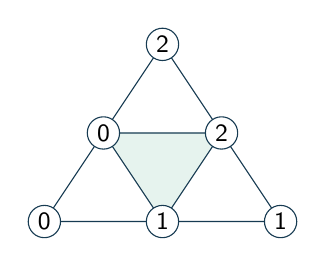
\begin{tikzpicture}[x=.75cm,y=.75cm]
\coordinate(A)at(0,0);\coordinate(B)at(4,0);\coordinate(C)at(2,3);\coordinate(D)at(2,0);\coordinate(E)at(3,1.5);\coordinate(F)at(1,1.5);
\fill[soft](D)--(E)--(F)--cycle;\draw[inkblue](A)--(B)--(C)--cycle (D)--(E)--(F)--cycle;
\foreach \p/\l in {A/0,B/1,C/2,D/1,E/2,F/0}{\node[draw=inkblue,circle,fill=white,inner sep=1.5pt,font=\small\sffamily] at (\p){\l};}
\end{tikzpicture}
\end{minipage}\begin{minipage}{.54\linewidth}\small
In dimension two, count incidences with edges labeled $0,1$. The lower-left triangle contributes two. The shaded triangle contributes one and carries all three labels. On the outer boundary just one edge has labels $0,1$.
\end{minipage}
\end{center}

\paragraph{Objects for Lean.} Store each $K_j$ and label/carrier array with explicit lengths and bounds; order vertex tuples to identify two copies of a facet. The incidence predicate for $(\sigma,\tau)$ scans the $j+1$ single deletions. Double count this Boolean over the rectangular product of cell and facet indices. Use the recursion $\operatorname{parity}(a+b)=\operatorname{parity}(\operatorname{parity}(a)+\operatorname{parity}(b))$ and test all claims about boundary carriers directly from the data. The conclusion about a geometric realization is the interpretation of the finite input contract. No oracle for recognizing triangulations or for sampling arbitrary real maps is used.

\section{Self-avoiding walks and finite Ising models}
\label{sec:models}

The square-grid walk illustrated in the survey and the Ising model in its physics section admit a common calculation. A spin correlation on a finite piece of the square grid can be bounded by counting walks between the two marked sites. We use polynomial identities and rational edge weights throughout.

\subsection{Counting walks without revisiting a vertex}

A walk of length $n$ starts at $(0,0)$ and is a word on the four unit coordinate directions. It is \emph{self-avoiding} if its $n+1$ partial-sum positions are distinct. Write $c_n$ for the count. Scan the $4^n$ words, compute integer coordinates in $[-n,n]$, and compare every pair of positions. In particular $c_n$ is a primitive recursive function.

\begin{theorem}[Finite square-lattice walk estimates]\label{result73}\label{thm:model-saw}
The initial values $c_0,\ldots,c_4$ are $1,4,12,36,100$. One has $c_{m+n}\le c_mc_n$ and
\[
  c_{1+3k+r}\le4\,25^k3^r \quad(0\le r<3),\qquad
  c_n\ge d_n,\quad d_0=1,\quad d_1=3,\quad d_{n+2}=2d_{n+1}+d_n .
\]
In particular $d_n\ge(1+\sqrt2)^n$. For every chosen block length $m\ge1$, writing $n=qm+s$ with $s<m$ gives $c_n\le c_m^q c_s$.
\end{theorem}
\begin{proof}
Split a self-avoiding walk at time $m$ and translate the second piece to the origin. The two pieces recover the whole walk and are each self-avoiding. This injection proves submultiplicativity, and iteration proves the block bound. After one step, each continuation has at most three choices because an immediate reversal revisits a vertex. On the square lattice, every nonempty closed walk has even length by coordinate parity. A nonbacktracking walk of length at most three therefore has no repeat. This gives the first four values. With four steps, a repeat in a nonbacktracking walk must be a square returning to the origin. There are eight such directed traversals, from the four possible first steps and two turning senses. Thus $c_4=4\cdot3^3-8=100$. After any nonempty prefix, append three nonbacktracking steps. Of their $27$ possible relative turn words, three consecutive left turns and three consecutive right turns return to the start of the last prefix edge. At most $25$ survive. Iterating this three-step estimate proves the upper bound.

For the lower bound allow east, north and south moves, and within each vertical column allow a monotone run. Such walks are self-avoiding, since each east move enters a new column. Conversely an east/north/south self-avoiding walk cannot reverse its vertical direction without an intervening east move. A column run of length $j$ has one choice at $j=0$ and two at $j>0$. For a transparent recurrence let $V=1+2z+2z^2+\cdots$ count the runs by length and let $D=\sum_n d_nz^n$ count the restricted walks. Decomposition at the first east step gives $D=V+zVD$. Since $(1-z)V=1+z$, multiplication gives $(1-2z-z^2)D=1+z$. This identity and all operations are read at any prescribed degree, truncating both tables there. Comparing coefficients yields the displayed recurrence. In the ordered quadratic integers put $u=1+\sqrt2$. We have $u^2=2u+1$, $d_0=1$, and $d_1\ge u$. Induction with the recurrence gives $d_n\ge u^n$. The integer recurrence itself supplies the lower bound in ordinary iPRA. If the quadratic comparison is desired, sign of $a+b\sqrt2$ for rational $a,b$ of opposite sign is decided by comparing $a^2$ with $2b^2$, with the sign determined by which term dominates.
\end{proof}

\subsection{Even subgraphs, cuts, and one-dimensional correlations}

Let $G=(V,E)$ be a finite undirected graph with indexed edges, allowing parallel edges. For a spin assignment $\sigma:V\to\{-1,1\}$, an edge $e=ij$ contributes weight $a_e$ if its endpoints agree and $b_e$ if they differ. Its configuration weight $W(\sigma)$ is the product. For $S\subseteq V$ put
\[
 Z_S=\sum_{\sigma}W(\sigma)\prod_{i\in S}\sigma_i,\qquad Z=Z_\varnothing .
\]
The boundary $\partial F$ of an edge mask $F$ is its set of odd-degree vertices. For $D\subseteq E$, write $D=\delta U$ if its edges are precisely those crossing from $U\subseteq V$ to $V\setminus U$. A cut here refers to the edge mask, with all repeated realizations as vertex subsets identified.

\begin{theorem}[High- and low-temperature expansions]\label{result74}\label{thm:model-ising}
Let $p_e=a_e+b_e$, $q_e=a_e-b_e$, and let $k(G)$ count all components, including isolated vertices. For arbitrary rational edge weights,
\begin{align*}
 2^{|E|}Z_S &=
 2^{|V|}\sum_{\partial F=S}\prod_{e\notin F}p_e\prod_{e\in F}q_e,\\
 Z &=2^{k(G)}\sum_{D\text{ a cut}}\prod_{e\notin D}a_e\prod_{e\in D}b_e .
\end{align*}
The first formula gives $Z_S=0$ if $S$ meets some component in an odd number of vertices. All equalities can be cleared of denominators.
\end{theorem}
\begin{proof}
Twice the edge weight is $p_e+q_e\sigma_i\sigma_j$. Expand the product over all edges by choosing the second term on $F$, and multiply by the inserted spins from $S$. The exponent of the spin at vertex $v$ is $d_F(v)+[v\in S]$. If any exponent is odd, flip the least-index spin with odd exponent to pair the terms with opposite signs. If all are even, every assignment contributes the same spin factor $1$. This proves the first formula. The sum of degrees in any component is twice its edge count, so no $F$ can realize the stated odd intersection. For the second formula, the disagreement edges of $\sigma$ are the cut from its negative-spin set. Two configurations give the same cut precisely when their pointwise product is constant on each component. Indeed at each edge the two endpoint products must agree, which propagates along paths. Each such componentwise constant choice gives an assignment with the required cut. Thus every cut contributes exactly $2^{k(G)}$ copies of its weight.
\end{proof}

\begin{corollary}[Open chain, ring and two-point functions]\label{result75}
For uniform weights $a,b$, put $p=a+b$, $q=a-b$. On a tree with $v\ge1$ vertices, $Z=2p^{v-1}$. For distinct vertices $x,y$ at distance $d$ in a tree and $a,b>0$, $Z_{\{x,y\}}/Z=(q/p)^d$. In particular these are exact formulas for an open chain. On the cycle of $n\ge3$ vertices,
\[
 Z=p^n+q^n,\qquad
 Z_{\{x,y\}}=q^d p^{n-d}+q^{n-d}p^d
\]
when the two arcs from $x$ to $y$ have lengths $d,n-d$.
\end{corollary}
\begin{proof}
A nonempty edge subset in a tree contains a leaf in a nontrivial component of that subset, so only the empty subset has empty boundary. A simple path from $x$ to $y$ is unique, since two distinct simple paths would contain a cycle. Its edge mask has boundary $\{x,y\}$. Symmetric difference adds vertex degrees modulo two, so any other mask with that boundary would differ by a nonempty even subgraph. Since $|E|=v-1$, substitution in Theorem~\ref{thm:model-ising} gives the two tree formulas. On a ring an even mask must take both or neither of the edges at each vertex, so the only even masks are the empty and the full mask. Toggling either with one of the two arcs between $x,y$ gives precisely the two masks with that boundary. The ring has equally many vertices and edges, yielding the stated expressions.
\end{proof}

\begin{theorem}[Rectangular duality with its boundary factor]\label{result76}
Take a rectangle of $w\times h$ unit square cells, $w,h\ge1$. Its grid graph $G$ has all sides of all cells as edges. The dual $G^*$ has one vertex per cell and one exterior vertex. An edge crosses each primal edge and joins its two incident faces, counting the exterior face along the boundary. If $Z_{G^*}^{+}$ fixes the exterior spin at $+1$, then
\[
 2^{|E|} Z_G(\mathbf a,\mathbf b)
    =2^{|V|}Z_{G^*}^{+}(\mathbf p,\mathbf q)
    =2^{|V|-1}Z_{G^*}(\mathbf p,\mathbf q).
\]
Moreover the grid has $2^{wh}$ even edge masks.
\end{theorem}
\begin{proof}
The mod-two sum of the boundaries of a chosen set of cells is even, since each individual cell boundary is even. Mark the chosen cells with negative spin and all other faces with positive spin. A primal edge survives the mod-two sum exactly when its two incident face spins disagree.

Conversely, given an even mask $F$, scan each column of cells from bottom to top. Starting with the bottom exterior bit zero, toggle the current bit each time the horizontal edge directly below the next cell belongs to $F$, assigning the new bit to that cell. This is the unique assignment reproducing $F$ on every horizontal edge except possibly the top boundary. Subtract its cell boundaries from $F$ modulo two. The residual mask is even and supported on the vertical columns and the top horizontal row. Those edges form a tree: the only horizontal moves are along the top path, with a single descending path attached at each top vertex. Consequently the residual is empty, by the leaf argument above. This gives an explicit bijection between all even masks and the $2^{wh}$ cell assignments with fixed exterior. The even-subgraph weights in Theorem~\ref{thm:model-ising} are now exactly the dual agreement and disagreement weights $p_e,q_e$. Finally global spin reversal pairs assignments of opposite exterior spin with equal weight. This proves both boundary normalizations.
\end{proof}

\subsection{A finite correlation estimate from self-avoidance}

\begin{proposition}[A finite-volume path bound]\label{result77}
In any finite subgraph of the square lattice with uniform weights $a\ge b>0$, put $t=(a-b)/(a+b)$. For distinct sites $x,y$ in the same component, let $d$ be their graph distance, let $v=|V|$, and put $k=\lfloor(d-1)/3\rfloor$. Then
\[
 0\le\frac{Z_{\{x,y\}}}{Z}\le\sum_{\ell=d}^{v-1}c_\ell t^\ell .
\]
If $25t^3<1$, an upper bound independent of $v$ is
\[
 \frac{4t(1+3t+9t^2)}{1-25t^3}(25t^3)^k .
\]
\end{proposition}
\begin{proof}
Cancel common factors in the high-temperature expressions. The ratio is
the sum of $t^{|F|}$ over masks with boundary $\{x,y\}$ divided by the sum
over even masks, whose empty term is $1$. Every numerator mask contains
a path from $x$ to $y$, since each component has an even number of odd
vertices. Select its least simple such path $P$ in a fixed word ordering.
Deleting the path edges gives an even mask $D$ disjoint from $P$, and
$(P,D)$ determines $F$. Thus the numerator is at most
$\sum_P t^{|P|}\sum_{D\text{ even}}t^{|D|}$, since all terms are
nonnegative. Paths of length $\ell$ from $x$ to $y$ translate into
distinct self-avoiding walks on the square lattice. This gives the first
bound. Group lengths by $\ell=1+3j+r$, $0\le r<3$. All such $j$ are at
least $k$. By Theorem~\ref{thm:model-saw} each full group contributes at
most $4t(1+3t+9t^2)(25t^3)^j$. For rational $0\le u<1$ the finite
sum of $u^j$ from $k$ to any $J\ge k$ is at most $u^k/(1-u)$ by
multiplication with $1-u$. This proves the second bound using only a
finite sum.
\end{proof}

\paragraph{Arithmetic and Lean implementation.}
For walks use a base-four direction word and length. Each coordinate prefix
is the difference of two finite direction counts, and self-avoidance is
a conjunction of comparisons of prefix pairs. Truncated power series for
$d_n$ use $n+1$ coefficients. For spins use one vertex bit per sign,
one edge bit per selected bond and a parity fold at each vertex for
\texttt{boundary}. The expansion proof is induction on the prefix
of indexed edges followed by the single-spin sign-reversing pairing.
After clearing denominators let $A$ bound $1,|a_e|,|b_e|$. Intermediate
absolute coefficient products are at most $(2A)^{|E|}$ and the crude
bound $2^{|V|+|E|}(2A)^{|E|}$ controls all expanded sums. For duality,
\texttt{fillCells} folds horizontal-edge bits along each of $w$
columns of height $h$. Test the residual tree and fixed-exterior spin
by Boolean scans. In the path bound choose $P$ by a search over
vertex words of length at most $v$; the disjoint union of its edges
with $D$ is the inverse on the image. This proves quantitative
statements for each finite input. For the relation with planar Ising
expansions see \href{https://arxiv.org/abs/1209.0951}{Cimasoni and
Duminil-Copin}.

\section{Lean formalization and the ProveIt boundary}\label{sec:lean}
\subsection{Checked statements in the archive}
Five standalone source files were checked with Lean 4.32.0. Their numerical inputs and the preceding encodings allow comparison with the arithmetic statements. The axiom reports below are Lean metatheoretic dependencies. In particular they describe the proofs of the Lean statements, not extra object axioms of iPRA.

\begin{center}\small\renewcommand{\arraystretch}{1.17}
\begin{tabular}{@{}p{.21\linewidth}p{.495\linewidth}>{\raggedright\arraybackslash}p{.22\linewidth}@{}}\toprule
File & Kernel-checked content & Axiom audit of named endpoints\\\midrule
\texttt{Bounded.lean} & Least numerical witness with sentinel, its range, success, minimality and a constructive existential equivalence. Executable Hall condition and zero-sum selector. & \texttt{propext}, \texttt{Quot.sound} for search\\
\texttt{WordCount.lean} & Derivation tree of $W_n=(a+b)^n$, then a soundness proof interpreting all rules over naturals. & None for certificate. The interpreted equality uses \texttt{propext}\\
\texttt{Handshaking.lean} & Finite double-sum interchange, weighted symmetric degree sum, $\sum_v d(v)=2e$ for a graph mask, and an explicit half of the odd-degree count. & None for all four reported theorems\\
\texttt{Kirkman.lean} & Seven days with five valid triples each, one attendance per pupil per day, and one meeting for every $x<y<15$. & None for all three theorems\\
\texttt{ThueMorse.lean} & Digit recurrences, scalar PR prefix coding, odd/even overlap descent, a bounded mismatch, aperiodicity, cube-freeness and prefix balance. & \texttt{propext}, \texttt{Quot.sound} for the reported endpoints\\\bottomrule
\end{tabular}
\end{center}
The word-count certificate uses a small equational language: the base and step constructors for powers and word counts, multiplication congruence, symmetry and transitivity, distributivity, and induction on equality of two terms. Its induction premises substitute zero and successor for the sole induction variable, leaving two free letter-count parameters. Reading these constructors as the corresponding iPRA rules is a rule-by-rule interpretation; distributivity is a derived semiring law. The other standalone files prove ordinary Lean propositions. The integral/series arguments, uniform hypergraph Ramsey theorem, hook formulas, polytope results and other results outside these endpoints have the human proofs and formalization plans in their respective sections.

\subsection{Constructing derivations in the repository's ordinary proof calculus}
The inspected repository revision is \texttt{b4de6f7a61a3fcf9740373b93089830f79e342f6}. Its \texttt{ConciseIPRA.PR} represents terms as \texttt{PTm n}, formulas by \texttt{Fm PTm n}, and derivations by a judgment of the form \(\Gamma\vdash[\mathrm{PRAAx}]\varphi\). Its \texttt{IPRADerivations} library supplies arithmetic and inference steps; its research packets have separate verification statuses. The combinatorics packet directory at this revision lists Bell numbers, Catalan numbers, Fibonacci--Lucas numbers, and finite Ramsey theory. For parameterized bijections use the following order of work.

\begin{enumerate}
\item \textbf{Define the representation terms.} Introduce powers, quotient, parity, masked size, lookup, padding and set difference. Express each table update with composition or primitive recursion. Use the pairing projections to pass multiple parameters to a bounded sum. For a new object give a Boolean validity term, domain bound and canonical decoding. Prove the two radix laws in Section~\ref{sec:found} using division with remainder; then iteration supplies lookup-after-write and prefix reconstruction. Translate the hypotheses on graphs, families, moves and covers into bounded Boolean terms by Lemma~\ref{lem:search}.
\item \textbf{Prove counting once.} Use \texttt{sum\_zero\_elim} to extract pointwise validity from zero violation totals; \texttt{Search.search\_found} to extract a successful witness; \texttt{strong\_ind} when all earlier indices are needed. The repository theorem \texttt{FiniteBijection.finite\_bijection} asks for four object derivations: the forward and reverse maps preserve bounds and valid objects, and each round trip is the identity on its own valid domain. It then identifies the two indicator sums. The prefix arguments in our bijective proofs establish precisely these obligations. When two valid encodings can denote the same object, restrict to canonical representatives or prove invariance and count the explicitly sized fibers.
\item \textbf{Illustration with Pr\"ufer.} Use one common numerical parameter packing $n$, initial graph and current live mask as needed. The source predicate tests a simple tree on $[n]$; its bound is $2^{\binom n2}$. The target predicate tests a length-$n-2$ base-$\max(2,n)$ word and $n\ge2$, bounded by $\max(2,n)^{n-2}$. Each encoder step chooses the first vertex with live degree one, emits its neighbor and erases it; the decoder takes the first live label absent from the unprocessed suffix. In the decoder's remaining tree the degree of each live label is one plus its number of suffix occurrences. The final two live labels have degree one. Adding the deleted edge proves the degree formula backwards and recovers the exact leaf choice forwards. Use the four resulting judgments as hypotheses to the bijection theorem; then replace the count of words by its radix power. Section~\ref{sec:graphs} proves the invariants independently of the representation.
\item \textbf{Illustration with variable-rank Ramsey.} For fixed final parameters $(h,c,m)$ first form $N=H_h(c,m)$. Write $B(j)$ for the sum, over rank-$j$ color tables on $H_j$ points, of indicators that all $m$-masks fail. Encode invalid table entries as zero contributions. The induction matrix can be $B(j)=0$ guarded by $1\le j\le h$ with $h,c,m,N$ as parameters. The induction step builds the pivot list, records the thinned colors and forms one smaller coloring. Apply the sum-zero rule to that coloring, recover its least homogeneous mask and lift it to the pivot labels. The rank proof in Section~\ref{sec:graphs} bounds every table in this use. The repository's \texttt{RamseyBounds.neighbor\_split} and \texttt{pascal\_bound} cover arithmetic steps for the graph bound; they have narrower conclusions than this new uniform hypergraph statement.
\item \textbf{Close each theorem.} Replace subtraction of signed quantities by addition of the positive and negative registers on opposite sides. Use only positive denominators when clearing a ratio. Prove the Boolean implication $\mathrm{Valid}\Rightarrow\mathrm{Check}$ for free parameter terms by these bounded inductions, turn its truth equation into the object implication, and universally close the parameters. Where the mathematical statement has an existential conclusion, introduce the numerical selector with its success proof. For analytic estimates the precision index is another numeric parameter and the witnesses are rational endpoints or mesh sizes. The final target is a closed object derivation \( []\vdash[\mathrm{PRAAx}]\varphi\).
\end{enumerate}
For exact reusable names, \texttt{lean/ProveItEndpoints.lean} lists references to the pinned modules. For example \texttt{Catalan.cat\_spec} supplies $(n+1)C_n=\binom{2n}{n}$ and \texttt{Vandermonde.vandermonde} uses a guarded binomial coefficient that vanishes above its row. The names and their source signatures were checked against the repository. The optional import file has not been built in the full ProveIt workspace during this study. The five standalone files were compiled separately; the transcript accompanies the archive.

\subsection{Source scope and further questions}
The starting article was read at revision 1384635198. The file \texttt{sources/direct-links.tsv} records its English article links from the introduction through ``See also,'' with their anchor text and enclosing section. \texttt{sources/theorem-map.tsv} matches result groups to these entry points. For example, the triangle-free maximum and the questions about intersecting and inclusion-incomparable families occur in the overview; the twelvefold enumeration and the two tableau counts are developed at immediate destinations. The group-action, zero-sum and Markov-tree arguments also supply consequences along these topics. The coverage is selective. Infinite Ramsey for arbitrary set-valued colorings, the full four-color theorem, and an infinite-volume two-dimensional Ising solution lie outside the proofs given here. The finite Ising identities in Section~\ref{sec:models} specify their graph and boundary conditions.

Three next questions follow directly from the proofs. Can the entire mask-level Pr\"ufer bijection be exported to \texttt{Prf PRAAx} with a single reusable deletion lemma? Can the two-cut sliding-window argument be replaced by an explicit iPRA parity certificate for arbitrary numbers of bead colors and the optimal cut bound? How much of the uniform Ramsey proof can share a single object-language lemma for lifting a homogeneous set through an order-preserving embedding?

\begin{thebibliography}{9}\small
\bibitem{overview} Wikipedia contributors. \emph{Combinatorics}, revision 1384635198. \href{https://en.wikipedia.org/w/index.php?title=Combinatorics\&oldid=1384635198}{Article snapshot}.
\bibitem{ipra} V. Reshetnikov and contributors. \emph{ProveIt}, Logic/PrimitiveRecursiveArithmetic. \href{https://github.com/VladimirReshetnikov/ProveIt/tree/b4de6f7a61a3fcf9740373b93089830f79e342f6/Logic/PrimitiveRecursiveArithmetic}{Pinned source tree} and \href{https://github.com/VladimirReshetnikov/ProveIt/tree/b4de6f7a61a3fcf9740373b93089830f79e342f6/Logic/PrimitiveRecursiveArithmetic/Derivations/Lean/IPRADerivations/Combinatorics}{individual derivations}.
\bibitem{alon} N. Alon. Combinatorial Nullstellensatz. \emph{Combinatorics, Probability and Computing} 8 (1999), 7--29. \href{https://www.math.tau.ac.il/~nogaa/PDFS/null2.pdf}{Author's paper}.
\bibitem{sokal} A. D. Sokal. The multivariate Tutte polynomial (alias Potts model) for graphs and matroids. \emph{Surveys in Combinatorics 2005}, 173--226. \href{https://arxiv.org/abs/math/0503607}{Author's preprint}.
\bibitem{thue} J.-P. Allouche and J. Shallit. The ubiquitous Prouhet--Thue--Morse sequence. In \emph{Sequences and Their Applications}, 1999, 1--16. \href{https://cs.uwaterloo.ca/~shallit/Papers/ubiq15.pdf}{Authors' paper}.
\end{thebibliography}

\clearpage
\section*{Index of proved results}
\phantomsection
\addcontentsline{toc}{section}{Index of proved results}
\markboth{Theorem index}{}
The statement number links to its proof. Each number can cover several related identities. The source concordance in the archive gives the corresponding article and explains the relationship.
\begin{multicols}{2}
\small\raggedcolumns\raggedright
\par\addvspace{.8em}\noindent{\bfseries\color{inkblue}What the finite statements mean in iPRA}\par\nopagebreak[4]
\noindent\hangindent=2.9em\hangafter=1\makebox[2.9em][l]{\hyperref[result01]{\ref*{result01}}}Bounded reflection and search\nobreak\hspace{.4em plus 1fill}\mbox{\pageref{result01}}\par
\noindent\hangindent=2.9em\hangafter=1\makebox[2.9em][l]{\hyperref[result02]{\ref*{result02}}}Counting fibers and cancelling signs\nobreak\hspace{.4em plus 1fill}\mbox{\pageref{result02}}\par
\noindent\hangindent=2.9em\hangafter=1\makebox[2.9em][l]{\hyperref[result03]{\ref*{result03}}}Weighted words and the geometric sum\nobreak\hspace{.4em plus 1fill}\mbox{\pageref{result03}}\par
\par\addvspace{.8em}\noindent{\bfseries\color{inkblue}Enumeration by reversible finite constructions}\par\nopagebreak[4]
\noindent\hangindent=2.9em\hangafter=1\makebox[2.9em][l]{\hyperref[result04]{\ref*{result04}}}Binomial identities\nobreak\hspace{.4em plus 1fill}\mbox{\pageref{result04}}\par
\noindent\hangindent=2.9em\hangafter=1\makebox[2.9em][l]{\hyperref[result05]{\ref*{result05}}}Compositions and Fibonacci identities\nobreak\hspace{.4em plus 1fill}\mbox{\pageref{result05}}\par
\noindent\hangindent=2.9em\hangafter=1\makebox[2.9em][l]{\hyperref[result06]{\ref*{result06}}}Twelvefold way, including empty sets\nobreak\hspace{.4em plus 1fill}\mbox{\pageref{result06}}\par
\noindent\hangindent=2.9em\hangafter=1\makebox[2.9em][l]{\hyperref[result07]{\ref*{result07}}}Stirling and Bell identities\nobreak\hspace{.4em plus 1fill}\mbox{\pageref{result07}}\par
\noindent\hangindent=2.9em\hangafter=1\makebox[2.9em][l]{\hyperref[result08]{\ref*{result08}}}A cancellation involution\nobreak\hspace{.4em plus 1fill}\mbox{\pageref{result08}}\par
\noindent\hangindent=2.9em\hangafter=1\makebox[2.9em][l]{\hyperref[result09]{\ref*{result09}}}Conjugation, Euler's product, and the Durfee square\nobreak\hspace{.4em plus 1fill}\mbox{\pageref{result09}}\par
\noindent\hangindent=2.9em\hangafter=1\makebox[2.9em][l]{\hyperref[result10]{\ref*{result10}}}Reflection and first return\nobreak\hspace{.4em plus 1fill}\mbox{\pageref{result10}}\par
\noindent\hangindent=2.9em\hangafter=1\makebox[2.9em][l]{\hyperref[result11]{\ref*{result11}}}Concrete Catalan families\nobreak\hspace{.4em plus 1fill}\mbox{\pageref{result11}}\par
\noindent\hangindent=2.9em\hangafter=1\makebox[2.9em][l]{\hyperref[result12]{\ref*{result12}}}Schr\"oder--Hipparchus numbers\nobreak\hspace{.4em plus 1fill}\mbox{\pageref{result12}}\par
\noindent\hangindent=2.9em\hangafter=1\makebox[2.9em][l]{\hyperref[result13]{\ref*{result13}}}Narayana refinement\nobreak\hspace{.4em plus 1fill}\mbox{\pageref{result13}}\par
\par\addvspace{.8em}\noindent{\bfseries\color{inkblue}An effective Catalan asymptotic}\par\nopagebreak[4]
\noindent\hangindent=2.9em\hangafter=1\makebox[2.9em][l]{\hyperref[result14]{\ref*{result14}}}Wallis bounds and relative error\nobreak\hspace{.4em plus 1fill}\mbox{\pageref{result14}}\par
\par\addvspace{.8em}\noindent{\bfseries\color{inkblue}Young tableaux, hook products and insertion}\par\nopagebreak[4]
\noindent\hangindent=2.9em\hangafter=1\makebox[2.9em][l]{\hyperref[result15]{\ref*{result15}}}Frame--Robinson--Thrall hook-length formula\nobreak\hspace{.4em plus 1fill}\mbox{\pageref{result15}}\par
\noindent\hangindent=2.9em\hangafter=1\makebox[2.9em][l]{\hyperref[result16]{\ref*{result16}}}Hook-content formula\nobreak\hspace{.4em plus 1fill}\mbox{\pageref{result16}}\par
\noindent\hangindent=2.9em\hangafter=1\makebox[2.9em][l]{\hyperref[result17]{\ref*{result17}}}Robinson--Schensted correspondence and Schensted's first-row theorem\nobreak\hspace{.4em plus 1fill}\mbox{\pageref{result17}}\par
\noindent\hangindent=2.9em\hangafter=1\makebox[2.9em][l]{\hyperref[result18]{\ref*{result18}}}Catalan permutation avoidance\nobreak\hspace{.4em plus 1fill}\mbox{\pageref{result18}}\par
\par\addvspace{.8em}\noindent{\bfseries\color{inkblue}Graphs, extremal problems and finite Ramsey theory}\par\nopagebreak[4]
\noindent\hangindent=2.9em\hangafter=1\makebox[2.9em][l]{\hyperref[result19]{\ref*{result19}}}Graph counts, handshaking and finite averages\nobreak\hspace{.4em plus 1fill}\mbox{\pageref{result19}}\par
\noindent\hangindent=2.9em\hangafter=1\makebox[2.9em][l]{\hyperref[result20]{\ref*{result20}}}Tur\'an, including equality\nobreak\hspace{.4em plus 1fill}\mbox{\pageref{result20}}\par
\noindent\hangindent=2.9em\hangafter=1\makebox[2.9em][l]{\hyperref[result21]{\ref*{result21}}}Bondy--Chv\'atal closure, Ore and Dirac\nobreak\hspace{.4em plus 1fill}\mbox{\pageref{result21}}\par
\noindent\hangindent=2.9em\hangafter=1\makebox[2.9em][l]{\hyperref[result22]{\ref*{result22}}}Berge parity, R\'edei and Camion\nobreak\hspace{.4em plus 1fill}\mbox{\pageref{result22}}\par
\noindent\hangindent=2.9em\hangafter=1\makebox[2.9em][l]{\hyperref[result23]{\ref*{result23}}}The Petersen graph\nobreak\hspace{.4em plus 1fill}\mbox{\pageref{result23}}\par
\noindent\hangindent=2.9em\hangafter=1\makebox[2.9em][l]{\hyperref[result24]{\ref*{result24}}}Finite Cayley graphs and Sabidussi's characterization\nobreak\hspace{.4em plus 1fill}\mbox{\pageref{result24}}\par
\noindent\hangindent=2.9em\hangafter=1\makebox[2.9em][l]{\hyperref[result25]{\ref*{result25}}}Two cyclic Gray listings\nobreak\hspace{.4em plus 1fill}\mbox{\pageref{result25}}\par
\noindent\hangindent=2.9em\hangafter=1\makebox[2.9em][l]{\hyperref[result26]{\ref*{result26}}}Euler's criterion\nobreak\hspace{.4em plus 1fill}\mbox{\pageref{result26}}\par
\noindent\hangindent=2.9em\hangafter=1\makebox[2.9em][l]{\hyperref[result27]{\ref*{result27}}}Pr\"ufer coding and Cayley's formula\nobreak\hspace{.4em plus 1fill}\mbox{\pageref{result27}}\par
\noindent\hangindent=2.9em\hangafter=1\makebox[2.9em][l]{\hyperref[result28]{\ref*{result28}}}K\H{o}nig, Hall and the deficiency formula\nobreak\hspace{.4em plus 1fill}\mbox{\pageref{result28}}\par
\noindent\hangindent=2.9em\hangafter=1\makebox[2.9em][l]{\hyperref[result29]{\ref*{result29}}}Regular bipartite graphs, edge coloring and transversals\nobreak\hspace{.4em plus 1fill}\mbox{\pageref{result29}}\par
\noindent\hangindent=2.9em\hangafter=1\makebox[2.9em][l]{\hyperref[result30]{\ref*{result30}}}Integral max-flow min-cut\nobreak\hspace{.4em plus 1fill}\mbox{\pageref{result30}}\par
\noindent\hangindent=2.9em\hangafter=1\makebox[2.9em][l]{\hyperref[result31]{\ref*{result31}}}Two-color graph Ramsey bounds\nobreak\hspace{.4em plus 1fill}\mbox{\pageref{result31}}\par
\noindent\hangindent=2.9em\hangafter=1\makebox[2.9em][l]{\hyperref[result32]{\ref*{result32}}}Finite multicolor hypergraph Ramsey theorem\nobreak\hspace{.4em plus 1fill}\mbox{\pageref{result32}}\par
\noindent\hangindent=2.9em\hangafter=1\makebox[2.9em][l]{\hyperref[result33]{\ref*{result33}}}A finite first-moment lower bound\nobreak\hspace{.4em plus 1fill}\mbox{\pageref{result33}}\par
\noindent\hangindent=2.9em\hangafter=1\makebox[2.9em][l]{\hyperref[result34]{\ref*{result34}}}Erd\H{o}s's sum-free subset bound\nobreak\hspace{.4em plus 1fill}\mbox{\pageref{result34}}\par
\end{multicols}
\newpage
\noindent{\sffamily\bfseries\large\color{inkblue}Index of proved results, continued}\par
\begin{multicols}{2}
\small\raggedcolumns\raggedright
\par\addvspace{.8em}\noindent{\bfseries\color{inkblue}Order, incidence, and extremal set systems}\par\nopagebreak[4]
\noindent\hangindent=2.9em\hangafter=1\makebox[2.9em][l]{\hyperref[result35]{\ref*{result35}}}Linear extensions and Mirsky's theorem\nobreak\hspace{.4em plus 1fill}\mbox{\pageref{result35}}\par
\noindent\hangindent=2.9em\hangafter=1\makebox[2.9em][l]{\hyperref[result36]{\ref*{result36}}}Dilworth's theorem\nobreak\hspace{.4em plus 1fill}\mbox{\pageref{result36}}\par
\noindent\hangindent=2.9em\hangafter=1\makebox[2.9em][l]{\hyperref[result37]{\ref*{result37}}}Erd\H{o}s--Szekeres\nobreak\hspace{.4em plus 1fill}\mbox{\pageref{result37}}\par
\noindent\hangindent=2.9em\hangafter=1\makebox[2.9em][l]{\hyperref[result38]{\ref*{result38}}}Finite distributive lattice representation\nobreak\hspace{.4em plus 1fill}\mbox{\pageref{result38}}\par
\noindent\hangindent=2.9em\hangafter=1\makebox[2.9em][l]{\hyperref[result39]{\ref*{result39}}}M\"obius inversion and product law\nobreak\hspace{.4em plus 1fill}\mbox{\pageref{result39}}\par
\noindent\hangindent=2.9em\hangafter=1\makebox[2.9em][l]{\hyperref[result40]{\ref*{result40}}}LYM, Sperner, and the general chain bound\nobreak\hspace{.4em plus 1fill}\mbox{\pageref{result40}}\par
\noindent\hangindent=2.9em\hangafter=1\makebox[2.9em][l]{\hyperref[result41]{\ref*{result41}}}Erd\H{o}s--Ko--Rado\nobreak\hspace{.4em plus 1fill}\mbox{\pageref{result41}}\par
\par\addvspace{.8em}\noindent{\bfseries\color{inkblue}Designs, finite planes, and error-correcting codes}\par\nopagebreak[4]
\noindent\hangindent=2.9em\hangafter=1\makebox[2.9em][l]{\hyperref[result42]{\ref*{result42}}}Descent, incidence counts, and derived designs\nobreak\hspace{.4em plus 1fill}\mbox{\pageref{result42}}\par
\noindent\hangindent=2.9em\hangafter=1\makebox[2.9em][l]{\hyperref[result43]{\ref*{result43}}}Fisher's inequality\nobreak\hspace{.4em plus 1fill}\mbox{\pageref{result43}}\par
\noindent\hangindent=2.9em\hangafter=1\makebox[2.9em][l]{\hyperref[result44]{\ref*{result44}}}Necessary Steiner triple parameters\nobreak\hspace{.4em plus 1fill}\mbox{\pageref{result44}}\par
\noindent\hangindent=2.9em\hangafter=1\makebox[2.9em][l]{\hyperref[result45]{\ref*{result45}}}Resolvable Steiner triple system on fifteen points\nobreak\hspace{.4em plus 1fill}\mbox{\pageref{result45}}\par
\noindent\hangindent=2.9em\hangafter=1\makebox[2.9em][l]{\hyperref[result46]{\ref*{result46}}}Planes of order q\nobreak\hspace{.4em plus 1fill}\mbox{\pageref{result46}}\par
\noindent\hangindent=2.9em\hangafter=1\makebox[2.9em][l]{\hyperref[result47]{\ref*{result47}}}Designs from affine and projective planes; the Fano plane\nobreak\hspace{.4em plus 1fill}\mbox{\pageref{result47}}\par
\noindent\hangindent=2.9em\hangafter=1\makebox[2.9em][l]{\hyperref[result48]{\ref*{result48}}}Hamming, Singleton, and Gilbert bounds\nobreak\hspace{.4em plus 1fill}\mbox{\pageref{result48}}\par
\noindent\hangindent=2.9em\hangafter=1\makebox[2.9em][l]{\hyperref[result49]{\ref*{result49}}}Perfect binary codes and their triples\nobreak\hspace{.4em plus 1fill}\mbox{\pageref{result49}}\par
\par\addvspace{.8em}\noindent{\bfseries\color{inkblue}Matroids, greedy optimization and the Tutte polynomial}\par\nopagebreak[4]
\noindent\hangindent=2.9em\hangafter=1\makebox[2.9em][l]{\hyperref[result50]{\ref*{result50}}}Rank and the greedy characterization\nobreak\hspace{.4em plus 1fill}\mbox{\pageref{result50}}\par
\noindent\hangindent=2.9em\hangafter=1\makebox[2.9em][l]{\hyperref[result51]{\ref*{result51}}}Graphic rank and minimum spanning forests\nobreak\hspace{.4em plus 1fill}\mbox{\pageref{result51}}\par
\noindent\hangindent=2.9em\hangafter=1\makebox[2.9em][l]{\hyperref[result52]{\ref*{result52}}}Rank expansion, deletion and contraction\nobreak\hspace{.4em plus 1fill}\mbox{\pageref{result52}}\par
\noindent\hangindent=2.9em\hangafter=1\makebox[2.9em][l]{\hyperref[result53]{\ref*{result53}}}The Potts, chromatic and Tutte identities\nobreak\hspace{.4em plus 1fill}\mbox{\pageref{result53}}\par
\par\addvspace{.8em}\noindent{\bfseries\color{inkblue}Polytope faces and exact kissing configurations}\par\nopagebreak[4]
\noindent\hangindent=2.9em\hangafter=1\makebox[2.9em][l]{\hyperref[result54]{\ref*{result54}}}Rational Birkhoff--von Neumann theorem\nobreak\hspace{.4em plus 1fill}\mbox{\pageref{result54}}\par
\noindent\hangindent=2.9em\hangafter=1\makebox[2.9em][l]{\hyperref[result55]{\ref*{result55}}}Dimension, facets, and edges of the Birkhoff polytope\nobreak\hspace{.4em plus 1fill}\mbox{\pageref{result55}}\par
\noindent\hangindent=2.9em\hangafter=1\makebox[2.9em][l]{\hyperref[result56]{\ref*{result56}}}Permutohedron\nobreak\hspace{.4em plus 1fill}\mbox{\pageref{result56}}\par
\noindent\hangindent=2.9em\hangafter=1\makebox[2.9em][l]{\hyperref[result57]{\ref*{result57}}}Simplex, cube, and cross-polytope\nobreak\hspace{.4em plus 1fill}\mbox{\pageref{result57}}\par
\noindent\hangindent=2.9em\hangafter=1\makebox[2.9em][l]{\hyperref[result58]{\ref*{result58}}}Small dimensions and explicit high-dimensional witnesses\nobreak\hspace{.4em plus 1fill}\mbox{\pageref{result58}}\par
\par\addvspace{.8em}\noindent{\bfseries\color{inkblue}Sumsets, restricted sums and zero-sum subsequences}\par\nopagebreak[4]
\noindent\hangindent=2.9em\hangafter=1\makebox[2.9em][l]{\hyperref[result59]{\ref*{result59}}}Three elementary estimates of Ruzsa type\nobreak\hspace{.4em plus 1fill}\mbox{\pageref{result59}}\par
\noindent\hangindent=2.9em\hangafter=1\makebox[2.9em][l]{\hyperref[result60]{\ref*{result60}}}The coefficient formula on a grid\nobreak\hspace{.4em plus 1fill}\mbox{\pageref{result60}}\par
\noindent\hangindent=2.9em\hangafter=1\makebox[2.9em][l]{\hyperref[result61]{\ref*{result61}}}Cauchy--Davenport and the restricted two-sum theorem\nobreak\hspace{.4em plus 1fill}\mbox{\pageref{result61}}\par
\noindent\hangindent=2.9em\hangafter=1\makebox[2.9em][l]{\hyperref[result62]{\ref*{result62}}}Erd\H{o}s--Ginzburg--Ziv, with the optimal threshold\nobreak\hspace{.4em plus 1fill}\mbox{\pageref{result62}}\par
\par\addvspace{.8em}\noindent{\bfseries\color{inkblue}Symmetries and impartial games}\par\nopagebreak[4]
\noindent\hangindent=2.9em\hangafter=1\makebox[2.9em][l]{\hyperref[result63]{\ref*{result63}}}Orbit--stabilizer and the orbit-counting lemma\nobreak\hspace{.4em plus 1fill}\mbox{\pageref{result63}}\par
\noindent\hangindent=2.9em\hangafter=1\makebox[2.9em][l]{\hyperref[result64]{\ref*{result64}}}P\'olya's inventory formula\nobreak\hspace{.4em plus 1fill}\mbox{\pageref{result64}}\par
\noindent\hangindent=2.9em\hangafter=1\makebox[2.9em][l]{\hyperref[result65]{\ref*{result65}}}Necklace and primitive necklace formulas\nobreak\hspace{.4em plus 1fill}\mbox{\pageref{result65}}\par
\noindent\hangindent=2.9em\hangafter=1\makebox[2.9em][l]{\hyperref[result66]{\ref*{result66}}}Normal play, the sum theorem, and Nim\nobreak\hspace{.4em plus 1fill}\mbox{\pageref{result66}}\par
\par\addvspace{.8em}\noindent{\bfseries\color{inkblue}Words, finite orbits and mixing}\par\nopagebreak[4]
\noindent\hangindent=2.9em\hangafter=1\makebox[2.9em][l]{\hyperref[result67]{\ref*{result67}}}Fine--Wilf\nobreak\hspace{.4em plus 1fill}\mbox{\pageref{result67}}\par
\noindent\hangindent=2.9em\hangafter=1\makebox[2.9em][l]{\hyperref[result68]{\ref*{result68}}}Thue--Morse, overlaps and equal powers\nobreak\hspace{.4em plus 1fill}\mbox{\pageref{result68}}\par
\noindent\hangindent=2.9em\hangafter=1\makebox[2.9em][l]{\hyperref[result69]{\ref*{result69}}}A ternary square-free word\nobreak\hspace{.4em plus 1fill}\mbox{\pageref{result69}}\par
\noindent\hangindent=2.9em\hangafter=1\makebox[2.9em][l]{\hyperref[result70]{\ref*{result70}}}Finite dynamics and a quantitative Markov-chain bound\nobreak\hspace{.4em plus 1fill}\mbox{\pageref{result70}}\par
\par\addvspace{.8em}\noindent{\bfseries\color{inkblue}Two cuts and a topological parity argument}\par\nopagebreak[4]
\noindent\hangindent=2.9em\hangafter=1\makebox[2.9em][l]{\hyperref[result71]{\ref*{result71}}}Two-color necklace splitting\nobreak\hspace{.4em plus 1fill}\mbox{\pageref{result71}}\par
\noindent\hangindent=2.9em\hangafter=1\makebox[2.9em][l]{\hyperref[result72]{\ref*{result72}}}Sperner's simplicial labeling lemma, with parity\nobreak\hspace{.4em plus 1fill}\mbox{\pageref{result72}}\par
\par\addvspace{.8em}\noindent{\bfseries\color{inkblue}Self-avoiding walks and finite Ising models}\par\nopagebreak[4]
\noindent\hangindent=2.9em\hangafter=1\makebox[2.9em][l]{\hyperref[result73]{\ref*{result73}}}Finite square-lattice walk estimates\nobreak\hspace{.4em plus 1fill}\mbox{\pageref{result73}}\par
\noindent\hangindent=2.9em\hangafter=1\makebox[2.9em][l]{\hyperref[result74]{\ref*{result74}}}High- and low-temperature expansions\nobreak\hspace{.4em plus 1fill}\mbox{\pageref{result74}}\par
\noindent\hangindent=2.9em\hangafter=1\makebox[2.9em][l]{\hyperref[result75]{\ref*{result75}}}Open chain, ring and two-point functions\nobreak\hspace{.4em plus 1fill}\mbox{\pageref{result75}}\par
\noindent\hangindent=2.9em\hangafter=1\makebox[2.9em][l]{\hyperref[result76]{\ref*{result76}}}Rectangular duality with its boundary factor\nobreak\hspace{.4em plus 1fill}\mbox{\pageref{result76}}\par
\noindent\hangindent=2.9em\hangafter=1\makebox[2.9em][l]{\hyperref[result77]{\ref*{result77}}}A finite-volume path bound\nobreak\hspace{.4em plus 1fill}\mbox{\pageref{result77}}\par
\end{multicols}

\end{document}
